%*******************************************************
%%% Thesis for Astrophysics & Cosmology thesis
%%% Alma Mater Studiorum - University of Bologna
%%% Author: Simone La Porta
%%% Created: March 2024
%*******************************************************


%%%%% DOCUMENT CLASS ************************************************************
\documentclass[print, final]{src/thesis}    % printing version
%\documentclass[final]{src/thesis}              % final electronic version)

%%%%% PREAMBLE ******************************************************************
% Loading files
%!TEX root = ../thesis.tex

%%%%%%%%%%%%%%% MATHEMATICS %%%%%%%%%%%%%%%
\usepackage{amsmath}    % mathematical typesetting
\usepackage{amsfonts}   % mathematics fonts
\usepackage{amssymb}    % mathematical symbols
\usepackage{amsthm}     % theorem-like environments
\usepackage{thmtools}   % extensions to theorem environments
\usepackage{array}      % array and matrices
\usepackage{siunitx}    % SI units
\usepackage{physics}    % physics


%%%%%%%%%%%%%%% GENERAL %%%%%%%%%%%%%%%
\usepackage[main=english, italian]{babel} % languages
\usepackage[utf8]{inputenc} % input encodings
\usepackage{enumitem} % layout of itemize, enumerate, description
\usepackage{accents}  % accents
\usepackage{appendix} % appendix
\usepackage{afterpage}  % commands expanded after the page
\usepackage[autostyle]{csquotes}  % quotations
\usepackage{fancyhdr} % page headers and footers
\usepackage{natbib} % bibliography support
\usepackage{lipsum} % dummy text
\usepackage{lmodern}  % latin modern fonts
\usepackage{microtype}  % typographical refinements
\usepackage{geometry} % manage document dimensions

%%%%%%%%%%%%%%% UTILS %%%%%%%%%%%%%%%
\usepackage{epsfig} % include eps
\usepackage{epstopdf} % convert eps to pdf
\usepackage{float}  % floating objects
\usepackage{graphicx} % support for graphics
\usepackage{longtable}  % tables over page boundaries
\usepackage{multicol} % multi columns
\usepackage{multirow} % tabular cells spanning multiple rows
\usepackage[final]{pdfpages}  % include pdf
\usepackage{relsize}  % font size relative to the current font size
\usepackage{subfig} % figures broken into subfigures
\usepackage{setspace} % space between lines
\usepackage{tcolorbox}  % coloured boxes
\usepackage{tikz} % tool to create graphic elements
\usepackage{url}  % url-sensitive line breaks
\usepackage{textcomp} % text companion font
\usepackage{xcolor} % color extensions
\usepackage{epigraph} % epigraph
\usepackage{listings} % code listings
\usepackage{mathrsfs} % script typestyle for uppercase letters
\usepackage{booktabs} % For professional looking tables
\usepackage[multiple]{footmisc} % multiple footnotes

% settings for the listings package
\lstset{frame=tb,
  language=Python,
  aboveskip=3mm,
  belowskip=3mm,
  showstringspaces=false,
  columns=flexible,
  basicstyle={\small\ttfamily},
  numbers=none,
  numberstyle=\tiny\color{gray},
  keywordstyle=\color{blue},
  commentstyle=\color{dkgreen},
  stringstyle=\color{mauve},
  breaklines=true,
  breakatwhitespace=true,
  tabsize=3
}

\usepackage[
    colorlinks=true,    % colored hyperlinks
    linkcolor=black,    % normal internal links
    citecolor=blue,     % bibliographical citations
    pdfpagemode=FullScreen, % how the file is opening in Acrobat
    pdftitle={
        Development of algorithms for strong lens analysis with PyTorch and TensorFlow
        },  % title of the file
    pdfauthor={Simone La Porta},    % author of the file
    pdfpagelayout=OneColumn % displays the document in one column, continuous scrolling
    ]{hyperref}     % support for hypertext

\usepackage[nameinlink, capitalise, english, italian]{cleveref}     % cross-referencing
% customize the way equation references are formatted when using the \cref command
\creflabelformat{equation}{(#2\textup{\textcolor{red}{#1}}#3)}

\usepackage{bookmark}   % manage pdf bookmarks

\urlstyle{same} % url same font of surrounding text	% packages
%!TEX root = ../thesis.tex

% Equations/math
\newcommand{\be}{\begin{equation}}  % start equation environment
\newcommand{\ee}{\end{equation}}    % end equation environment
\newcommand{\benn}{\begin{equation*}}   % start unnumbered equation environment
\newcommand{\eenn}{\end{equation*}}     % end unnumbered equation environment
\newcommand{\ba}{\begin{align}} % start align environment
\newcommand{\ea}{\end{align}}   % end align environment


% Tikz figures and utilities
\newcommand{\SF}{1}	% Scaling factor
\newcommand{\TS}{\normalsize}	% Text size
\newcommand{\lw}{0.7pt}	% Line width
\newcommand{\TSTick}{\small}	% Text size axis labels
\usetikzlibrary{arrows}	% Arrows library
\usetikzlibrary{patterns}	% Patterns library
\usetikzlibrary{decorations.markings}	% Decorations library
\usetikzlibrary{shadings}	% Shadings library
\usetikzlibrary{shapes}	% Shapes library


% Custom item headers or labels: bold, numbered header with the provided text, and the text that follows will not be indented, starting on a new line
% Usage: \itemheader{Some Text}
\newcommand{\itemheader}[1]{~\\ \noindent\textbf{#1.}\ \ }


% Same as before but starting on a new page
% Usage: \itemheaderNewpage{Some Text}
\newcommand{\itemheaderNewpage}[1]{\newpage \noindent\textbf{#1.}\ \ }


% Styled contribution block with a numbered title, and the provided content. The numbering will be in Roman numerals and increment with each usage of the \contribution command. The entire block is enclosed in a colored box to make it stand out.
% Usage: \contribution{Some Contribution Text}{Some Content}
\newcommand{\contribution}[2]{\refstepcounter{ContNum}#2 \vspace*{2.1mm}\begin{tcolorbox}[colback=black!2!white,colframe=black!20!white] \textbf{Contribution \Roman{ContNum}.} {\em #1} \end{tcolorbox}\vspace*{2.1mm}}


% Styled box with the provided objective text. The text will be formatted in italics, and the entire objective will be enclosed in a colored box to make it stand out.
% Usage: \objective{Some Objective Text}
\newcommand{\objective}[1]{\begin{tcolorbox}[colback=black!2!white,colframe=black!20!white] {\em #1} \end{tcolorbox}}


% Include a PDF document in the document, but only if the \ifprint condition is false.
% Usage: \cover{pdf file}
\newcommand{\cover}[1]{\ifprint{}\else\includepdf[pages=-]{#1}\cleardoublepage\fi}


% Empty page command: creates a blank page with no header or footer, and skip the page number.
\newcommand\blankpage{\null\thispagestyle{empty}\addtocounter{page}{-1}\newpage}


\newcommand{\ie}{i.e. } % id est formatted
\newcommand{\eg}{e.g. } % exempli gratia formatted	% custom commands
%!TEX root = ../thesis.tex


\usepackage{mathtools}  % extension of the amsmath package
\usepackage{xparse}     % custom document commands with more advanced and flexible syntax

%%%% BRACKETS **************************************************************
\newcommand{\bc}[1]{\left\lbrace #1 \right\rbrace}  % curly brackets adjusted auto
\newcommand{\bp}[1]{\left( #1 \right)}              % parentheses adjusted auto
\newcommand{\bs}[1]{\left[ #1 \right]}              % square brackets adjusted auto


%%%% GREEK LETTERS **************************************************************

\def\A{\Alpha}	% alpha
\def\a{\alpha}
\def\B{\Beta}	% beta
\def\b{\beta}
\def\c{\chi}	% chi
\def\G{\Gamma}	% gamma
\def\g{\gamma}
\def\D{\Delta}	% delta
\def\d{\delta}
\def\e{\epsilon}	% epsilon
\def\ve{\varepsilon}	% varepsilon
\def\F{\Phi}	% phi
\def\f{\phi}
\def\vf{\varphi}	% varphi
\def\h{\eta}
\def\T{\Theta}	% theta
\def\t{\theta}
\def\vt{\vartheta}	% vartheta
\def\k{\kappa}	% kappa
\def\L{\Lambda}	% lambda
\def\l{\lambda}
\def\m{\mu}	% mu
\def\n{\nu}	% nu
\def\O{\Omega}	% omega
\def\o{\omega}
\def\vp{\varpi}	% varpi
\def\P{\Psi}	% psi
\def\p{\psi}
\def\r{\rho}	% rho
\def\S{\Sigma}	% sigma
\def\s{\sigma}
\def\vs{\varsigma}	% varsigma
\def\X{\Xi}	% xi
\def\x{\xi}
\def\z{\zeta}	% zeta

% Scientific notation with a centered dot and a non-italicized exponent.
% Usage: number \pwr{exponent}
\newcommand{\pwr}[1]{\cdot10^{\textrm{#1}}}


%%%% UNITS **************************************************************
\DeclareSIUnit\year{yr}	% year
\DeclareSIUnit\parsec{pc}	% parsec
\DeclareSIUnit\msun{M_{\odot}}	% solar mass
\DeclareSIUnit\pixel{pix}	% pixel



\DeclareMathOperator{\arcsinh}{arcsinh}	% inverse hyperbolic sine
\DeclareMathOperator*{\argmin}{arg\,min}	% argmin	% custom mathematics

%\usepackage{showframe} % page-layout diagram


%%%%% DOCUMENT DETAILS **********************************************************
\author{Simone La Porta}
\title{Applications of automatic differentiation in gravitational lensing}
\makeatletter

\AtBeginDocument{\RenewCommandCopy\qty\SI}	% fix for siunitx and siunitx-quantity
\NewDocumentCommand{\anote}{}{\makebox[0pt][l]{$^*$}}	% add a note to tables
%%%% MAIN DOCUMENT *************************************************************
\begin{document}
\selectlanguage{english}
\pagenumbering{roman}
\thispagestyle{empty}

%%%%% FRONT MATTERS *************************************************************
\cover{img/cover_front.pdf}    % Add front cover if the option 'print' is not used.

% Color bleau de france for title and thumb index
%\definecolor{thumbcolor}{rgb}{0.19, 0.55, 0.91}
%\definecolor{titlecolor}{rgb}{0.19, 0.55, 0.91}

% Color black for title and thumb index
\definecolor{thumbcolor}{rgb}{0, 0, 0}
\definecolor{titlecolor}{rgb}{0, 0, 0}


%%%%% TITLEPAGE ***********************************
\thispagestyle{empty}
\newgeometry{
    left    =   25mm,
    right   =   20mm,
    top     =   20mm,
    bottom  =   20mm,
    bindingoffset   =   5mm
    }

\begin{center}
    \fontsize{18pt}{18pt}\selectfont
    \textbf{Alma Mater Studiorum - Università di Bologna}
    \par\noindent\hrulefill\vspace{2.5mm}
    
    \Large{School of Science \\ Department of Physics and Astronomy \\ Master Degree Programme in Astrophysics and Cosmology}
    
    \vspace{70mm}
    
    \fontsize{25pt}{25pt}{\textbf{Applications of automatic differentiation in gravitational lensing}}

    \vspace{5mm}
    
    Graduation Thesis
    
    \vspace{5mm}
    
    March 15, 2024
    
    \vfill
    
    \begin{minipage}[t]{0.34\textwidth}
        \begin{flushleft}
            {\fontsize{16pt}{16pt}{Presented by: \\ \vspace{1mm} \textbf{Simone La Porta}}}
        \end{flushleft}
    \end{minipage}
    \begin{minipage}[t]{0.64\textwidth}
        \begin{flushright}
            {\fontsize{16pt}{16pt} {Supervisor: \\ \vspace{1mm} \textbf{Chiar.mo Prof. Lauro Moscardini}}} \\
            \vspace{5mm}
            {\fontsize{16pt}{16pt} {Co-supervisor: \\ \vspace{1mm} \textbf{Dott. Massimo Meneghetti}}}
        \end{flushright}
    \end{minipage}
        
    \vspace{10mm}\noindent\hrulefill\vspace{3mm}
    
    \Large{Academic year 2022-2023 \\ Graduation date V}
\end{center}
\restoregeometry
\afterpage{\blankpage}

%%%%% EPIGRAPH ***********************************
\thispagestyle{empty}
\section*{}
\vspace{20ex}
\doublespacing
\epigraph{\textit{Nature uses only the longest threads to weave her patterns, so that each small piece of her fabric reveals the organization of the entire tapestry}}{Richard P. Feynman}
\afterpage{\blankpage}

\singlespacing

\setcounter{page}{1}

%%%%% ABSTRACT ***********************************
\chapter*{Abstract}
\addcontentsline{toc}{chapter}{Abstract}
\markboth{Abstract}{Abstract}
\pagestyle{empty}

Gravitational lensing, a remarkable consequence of Einstein's theory of general relativity, provides a unique opportunity to explore the fundamental properties of the universe by studying the distortions caused by massive objects on the path of light rays. However, analyzing and modeling gravitational lenses poses many challenges, due to the complex nature of the lensing effects and the vast amount of observational data and computational resources required.

The primary objective of this thesis is to address these challenges by developing advanced Python algorithms based on differentiable programming paradigm, leveraging the capabilities of PyTorch and TensorFlow frameworks to enable precise modeling and analysis of gravitational lenses. By employing parametric models, these algorithms exploit automatic differentiation to backpropagate errors and compute gradients of a loss function, facilitating the optimization of high-dimensional parameter spaces. 
Through the training of these parametric models, relevant features can be extracted and key parameters of the lensing system can be estimated. The resulting models can then be applied to real observational data, improving the characterization and classification of strong lenses with enhanced accuracy and efficiency.

The use of PyTorch and TensorFlow in the implementation of these algorithms allows efficient utilization of modern computational resources, such as GPUs, to handle the inherent computational complexity involved in strong lens analysis. Furthermore, the flexibility and extensibility of these frameworks enable seamless integration with other astrophysical and computational tools, facilitating a comprehensive and robust analysis of strong lenses.

The structure of this thesis is the following: an introduction to the main concepts of cosmology and gravitational lensing theory is presented in \cref{chap:cosmology,chap:gravitational_lensing}, followed by an extensive description of the most important lens models in \cref{chap:lens_models}. \Cref{chap:algorithms} describes the differentiable programming paradigm, its characteristics, and some examples of algorithms to model and analyze gravitational lenses and light sources. Finally, \cref{chap:applications} specifically focus on the application of differentiable programming and automatic differentiation methods to microlensing and strong lensing optimization problems. Finally, an example of surface brightness fitting is presented as a means to derive the shape and ellipticity of a galaxy, fundamental information for performing weak lensing measurements.

%%%%% SOMMARIO ***********************************
\selectlanguage{italian}
\chapter*{Sommario}
\addcontentsline{toc}{chapter}{Sommario}
\markboth{Sommario}{Sommario}
\pagestyle{empty}


Il lensing gravitazionale, una straordinaria conseguenza della teoria della relatività generale di Einstein, offre un'opportunità unica di esplorare le proprietà fondamentali dell'universo, studiando le distorsioni causate da oggetti massicci sul percorso dei raggi luminosi. Il lensing gravitazionale forte, in particolare, che si manifesta come immagini multiple altamente amplificate e distorte di sorgenti di background, offre preziose indicazioni sulla distribuzione della materia oscura e sulla formazione delle strutture cosmiche. Tuttavia, analizzare e modellare con precisione le lenti gravitazionali forti presenta varie difficoltà, a causa della natura complessa degli effetti di lensing e della vasta quantità di dati osservativi richiesti, oltre alle grandi risorse computazionali necessarie.
L'obiettivo principale di questo lavoro di tesi è quello di affrontare tali questioni sviluppando algoritmi Python avanzati per la precisa modellizzazione e analisi di lenti gravitazionali forti, fondati su tecniche di programmazione differenziabile, implementate utilizzando i framework PyTorch e TensorFlow.
Utilizzando modelli parametrici, questi algoritmi sfruttano la differenziazione automatica per retropropagare gli errori e calcolare i gradienti di una funzione di costo, facilitando l'ottimizzazione nello spazio dei parametri.
Attraverso l'implementazione in tali modelli parametrici, è possibile estrapolare le caratteristiche rilevanti e stimare i parametri chiave del sistema in esame. I modelli risultanti possono essere applicati a dati osservativi reali, migliorando la caratterizzazione e la classificazione delle lenti con maggiore precisione ed efficienza.
L'uso di PyTorch e TensorFlow nell'implementazione di questi algoritmi consente di utilizzare in modo efficiente le moderne risorse di calcolo, come le GPU, per gestire la complessità computazionale intrinseca all'analisi delle lenti forti. Inoltre, la flessibilità e l'estensibilità di questi framework consentono una perfetta integrazione con altri strumenti astrofisici e di calcolo, facilitando un'analisi completa e robusta.

La struttura di questa tesi è la seguente: nei \cref{chap:cosmology,chap:gravitational_lensing} viene presentata un'introduzione ai concetti principali della cosmologia e della teoria delle lenti gravitazionali, seguita da un'ampia descrizione dei più importanti modelli di lente nel \cref{chap:lens_models}. Il \Cref{chap:algorithms} descrive il paradigma della programmazione differenziabile, le sue caratteristiche e alcuni esempi di algoritmi per modellare e analizzare le lenti gravitazionali. Il \cref{chap:applications} si concentra specificamente sull'applicazione dei metodi di differenziazione automatica a problemi di ottimizzazione di microlensing e di lensing forte. Infine, viene presentato un esempio di analisi della brillanza superficiale per derivare la forma e l'ellitticità di una galassia, informazioni fondamentali per effettuare misurazioni di weak lensing.


\onehalfspacing

\selectlanguage{english}
%\cleardoublepage

%%%%% TOC ***********************************
\pdfbookmark{\contentsname}{Contents}
\tableofcontents

%\newpage

%%%%% GLOSSARY ***********************************
%\newenvironment{Nomen}
    {\vspace*{-3mm}\begin{center}
    \begin{longtable}{p{.1\textwidth} p{.83\textwidth}}
    }
    {
    \end{longtable}
    \end{center}\vspace*{-1.2cm}
    }
\newcommand{\AddSymbol}[2]{#1 & #2 \\}




%*********************************************************************************%
\chapter*{List of symbols}
\addcontentsline{toc}{chapter}{List of symbols}
\markboth{List of symbols}{List of symbols}

%*********************************************************************************%

\section*{Greek symbols}

\begin{Nomen}
\AddSymbol{$\alpha$}{What $\alpha$ is}
\AddSymbol{$\beta$}{What $\beta$ is}
\AddSymbol{$\gamma$}{What $\gamma$ is}
\AddSymbol{$\delta$}{What $\delta$ is}
\end{Nomen}


%*********************************************************************************%
\section*{Roman symbols}

\begin{Nomen}
\AddSymbol{$a$}{Description of $a$}
\AddSymbol{$b$}{Description of $b$}
\AddSymbol{$C$}{Description of $C$}
\AddSymbol{$D_a$}{Description of $D_a$}
\end{Nomen}


%*********************************************************************************%
\section*{Sub- and superscripts}

\begin{Nomen}
\AddSymbol{$\dot{(\cdot)}$}{First time derivative}
\AddSymbol{$\ddot{(\cdot)}$}{Second time derivative}
\AddSymbol{$\hat{(\cdot)}$}{Explain the reader what this means}
\AddSymbol{$(\cdot)_0$}{Explain the reader what this means}
\end{Nomen}


%*********************************************************************************%
\section*{Acronyms}

\begin{Nomen}
\AddSymbol{CoM}{Center of mass}
\AddSymbol{CoR}{Coefficient of restitution}
\end{Nomen}


%*********************************************************************************%
%\newpage
\section*{Operators and letter-like symbols}



%\thispagestyle{empty}


%\cleardoublepage

%%%%% LIST OF FIGURES *****************************
\pdfbookmark{\contentsname}{List of Figures}
\addcontentsline{toc}{chapter}{\listfigurename}
\listoffigures
%\cleardoublepage


%%%%% LIST OF TABLES *****************************
\pdfbookmark{\contentsname}{List of Tables}
\addcontentsline{toc}{chapter}{\listtablename}
\listoftables


%%%%% MAIN MATTER ***********************************
\isstarredchapterfalse	% normal chapter: YES thumb index
\cleardoublepage
\thispagestyle{empty}
\setcounter{page}{1}
\pagenumbering{arabic}
\pagestyle{fancy}

% *************************************************************
%%%%% CHAPTER 1: INTRODUCTION %%%%%
\chapter[Cosmological background]{Cosmological background}
\label{chap:cosmology}

% *************************************************************
%%%%% SECTION 1.1: HISTORY %%%%%
\section{History}
\label{sec:history}
Throughout history, questions surrounding the origin, age, and size of the universe have fascinated humans. Plato believed in a Universe that remains constant, envisioning it as an entity that was created perfect, unaging, and free from decay \citep{cornford_platos_2010}. This view of a static universe prevailed for more than two millennia, and it was so entrenched in cosmological thinking that even Albert Einstein initially subscribed to it. To reconcile his field equations of general relativity with the notion of a static universe, Einstein introduced the cosmological constant, a term that provided a mathematical means to allow for static solutions to his equations \citep{einstein_kosmologische_1917}.

However, the early 20th century brought discoveries that challenged the long-standing paradigm of a static universe. Vesto Slipher made pivotal observations, noting that most galaxies recede from the Milky Way at high velocities. Building on this foundation, Edwin Hubble, in the 1920s, conducted an analysis of the escape velocities of distant galaxies, leading to a groundbreaking discovery. Hubble observed that the farther away galaxies are, the faster they appear to be moving away. He plotted the radial velocities of these galaxies against their distances and found that the data could be best described by a straight line, indicating a linear relationship (\cref{fig:hubble}).

\begin{figure}
    \centering
    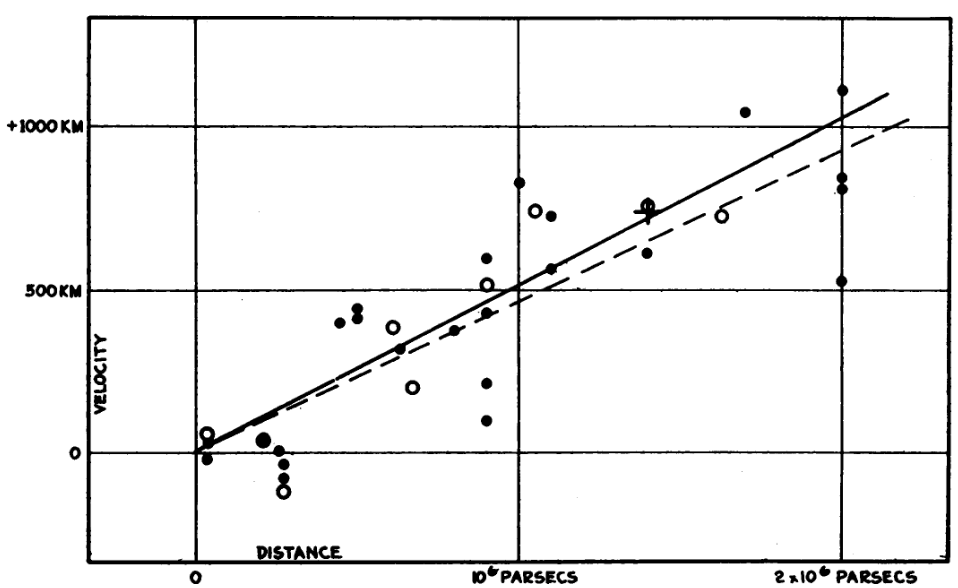
\includegraphics[width=0.8\linewidth, keepaspectratio]{img//chapter1/hubble.png}
    \caption[Hubble's Law: radial velocities of Extra-Galactic Nebulae]{Radial velocities, corrected for solar motion, plotted against distances estimated from involved stars and mean luminosities of nebulae in a cluster.\\\small{Credits: \cite{hubble_relation_1929}.}}
    \label{fig:hubble}
\end{figure}

Hubble's choice of a linear fit was influenced by his belief in the predictions of Friedmann's equations, which are solutions to Einstein's field equations of general relativity and suggest an expanding universe. Hubble's analysis and the linear relationship he identified, the basis for what is now known as \emph{Hubble's Law}, marked a fundamental shift in the understanding of the universe. It provided strong evidence for an expanding Universe, a concept that fundamentally contradicted the long-held belief in a static cosmos. This discovery not only revolutionized cosmology, but also led Einstein to reconsider the cosmological constant he had introduced.

The receding velocity $v$ of a galaxy leads to a Doppler shift in the galaxy's spectrum, observable as a redshift $z$:
\be
\label{eq:1.1}
v (r) = c \frac{\D \l}{\l} = c z = H_0 r \,,
\ee
where $H_0$ is the proportionality constant, subsequently named after Hubble, for which, in 1929 he published \citep{hubble_relation_1929} a value of
\be
\label{eq:1.2}
H_0 = \SI{530}{\kilo\meter\per\second\per\mega\parsec} \,,
\ee
much different from the current value \citep{tully_hubble_2023} of
\be
\label{eq:1.3}
H_0 = \SI[separate-uncertainty=true]{74.6 \pm 0.8}{\kilo\meter\per\second\per\mega\parsec} \,.
\ee

The unit of the Hubble constant is chosen according to the relation between escape velocity and
distance, but actually it has the unit of an inverse time, representing the age of the universe in a uniformly expanding model:
\be
\label{eq:1.4}
\tau_0 = H_0^{-1} \approx 13.9\pwr{9} \si{\year} \,.
\ee

% *************************************************************
%%%%% SECTION 1.2: FRIEDMANN'S EXPANSION EQUATIONS %%%%%
\section{Friedmann Equations}
\label{sec:friedmann_eq}


%%%%%%%%%%%%%%%%%%%%%%%%%%%%%%%%%%%%%%%%%%%%%%%%%%%%%%%
%%%%% Expansion rate %%%%%
%%%%%%%%%%%%%%%%%%%%%%%%%%%%%%%%%%%%%%%%%%%%%%%%%%%%%%%
\subsection{Expansion rate}
\label{subsec:exp_rate}
According to the \emph{Cosmological Principle}, on sufficiently large scales, the universe is homogeneous and isotropic. Considering a sphere with homogeneous density and a test particle at location $\vec{x}$, and introducing a spherical coordinate system that is allowed to expand with time, due to the cosmological principle, the expansion and the time-dependent position $\vec{r}(t)$ can be expressed by
\be
\label{eq:1.5}
\vec{r} (t) = a (t) \vec{x} \,,
\ee
where $a (t)$ is the \emph{cosmic scale factor}, which does not depend only on time. For $t_0 = \mathrm{today}$, the scale factor is conventionally set to $a(t_0) = 1$. Scalar quantities $r, x$ can be used instead of $\vec{r}, \vec{x}$ due to isotropy.

The velocity of a test particle caused by cosmic expansion is
\be
\label{eq:1.6}
v(r,t) = \frac{\dd{r(t)}}{\dd{t}} = \frac{\dd{a(t)}}{\dd{t}} x = \frac{\dot{a} (t)}{a(t)} r = H(t) r \,,
\ee
which leads to the definition of the \emph{Hubble parameter}, used to quantify the relative expansion rate of the universe
\be
\label{eq:1.7}
H(t) \equiv \frac{\dot{a} (t)}{a(t)} \,,
\ee
whose value in the present epoch, $H(t_0) = H_0$, is the \emph{Hubble constant}, expressed in \cref{eq:1.3}.


%%%%%%%%%%%%%%%%%%%%%%%%%%%%%%%%%%%%%%%%%%%%%%%%%%%%%%%
%%%%% Dynamics of the expansion %%%%%
%%%%%%%%%%%%%%%%%%%%%%%%%%%%%%%%%%%%%%%%%%%%%%%%%%%%%%%
\subsection{Dynamics of the expansion}
\label{subsec:exp_dyn}
To derive the Friedmann Equations and to study the evolution of the scale factor $a (t)$, to better understand the development of the universe, one has to start from Einstein field's equation, that describes the geometry of space-time:
\be
\label{eq:1.8}
R_{\m \nu} - \frac{1}{2} R g_{\m \nu} + g_{\m \nu} \L = \frac{8 \pi G}{c^4} T_{\m \nu} \,,
\ee
where $R_{\m \nu}$ and $R$ are the Ricci tensor and Ricci scalar, respectively, $\L$ is the \emph{cosmological constant} and $T_{\m \nu}$ is the \emph{energy-momentum tensor}, which includes all contributions of energy and acts as the source of gravity.

The energy-momentum tensor of the universe is that of a homogeneous perfect fluid, characterized by its density $\r (t)$ and pressure $p (t)$. Using the Robertson-Walker metric to describe homogeneity and isotropy, the Einstein's equations simplify to the \emph{Friedmann equations} \citep{friedman_uber_1922,friedmann_uber_1924}:
\begin{subequations}
\begin{align}
    \label{eq:1.9a}
    H (t)^2 &= \bp{\frac{\dot{a}}{a}}^2 = \frac{8 \pi G}{3} \r + \frac{\L c^2}{3} - \frac{K c^2}{a^2} \,,
    \\[2ex]
    \label{eq:1.9b}
    \frac{\ddot{a}}{a} &= - \frac{4 \pi G}{3} \bp{\r + \frac{3 p}{c^2}} + \frac{\L c^2}{3} \,,
\end{align}
\end{subequations}
where $K$ is a constant parameter that defines the curvature of spatial surfaces:
\begin{itemize}
    \item $K = -1$ means open, hyperbolic space (\ie infinite) with negative curvature;
    \item $K = 0$ means flat, Euclidean space;
    \item $K = 1$ means closed, spherical space with positive curvature.
\end{itemize}

It is then possible to split up the density $\r$ into
\begin{subequations}
\begin{align}
    \label{eq:1.10a}
    \r_m (t) = \r_{m,0} a(t)^{-3} \quad &\Rightarrow \quad \textrm{non-relativistic matter} \,,
    \\
    \label{eq:1.10b}
    \r_r (t) = \r_{r,0} a(t)^{-4} \quad &\Rightarrow \quad \textrm{relativistic matter} \,.
\end{align}
\end{subequations}

Furthermore, by defining the constant vacuum energy density $\r_\L = \frac{\L}{8 \pi G}$ and the critical density $\r_{cr} = \frac{3 H_0^2}{8 \pi G}$, it is convenient to introduce dimensionless density parameters for matter, radiation and vacuum energy:
\be
\label{eq:1.11}
\O_m = \frac{\r_m}{\r_{cr}} \,, \quad\quad\quad \O_r = \frac{\r_r}{\r_{cr}} \,, \quad\quad\quad \O_\L = \frac{\r_\L}{\r_{cr}} = \frac{\L}{3 H_0^2} \,.
\ee

Finally, introducing the curvature parameter
\be
\label{eq:1.12}
\O_K = - \frac{K c^2}{H_0^2} = 1 - (\O_m + \O_r + \O_\L) \,,
\ee
and subtracting \cref{eq:1.9a} from \cref{eq:1.9b}:
\be
\label{eq:1.13}
 H (t)^2 = \bs{\frac{\dot{a}(t)}{a(t)}}^2 = H_0^2 \bs{\O_r a(t)^{-4} + \O_m a(t)^{-3} + \O_K a(t)^{-2} + \O_\L} \,.
\ee

\Cref{eq:1.13} is a fundamental equation that completely describes the expansion of the universe and contains all the information about geometry, matter, and energy content.

\begin{figure}
    \centering
    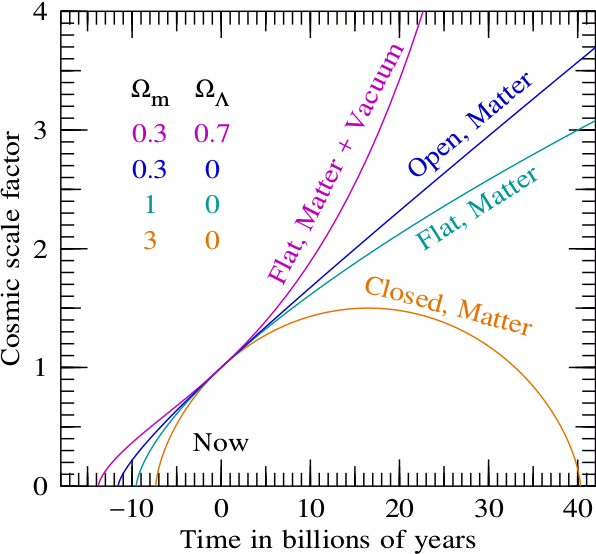
\includegraphics[width=0.65\linewidth, keepaspectratio]{img//chapter1/scalefactort.png}
    \caption[Temporal evolution of the cosmic scale factor]{Numerical solutions for \cref{eq:1.13} for different cosmological models.\\\small{Credits: \cite{hamilton_lecture_2019}.}}
    \label{fig:scalefactor}
\end{figure}


%%%%%%%%%%%%%%%%%%%%%%%%%%%%%%%%%%%%%%%%%%%%%%%%%%%%%%%
%%%%% Cosmological distances %%%%%
%%%%%%%%%%%%%%%%%%%%%%%%%%%%%%%%%%%%%%%%%%%%%%%%%%%%%%%
\subsection{Cosmological distances}
\label{subsec:dist}
In a curved space-time, there are various ways to define the distance between two points. Setting $P_0$ as the origin of a set of polar coordinates $(r, \t, \f)$ and assuming $\dd{t} = \dd{\f} = \dd{\t} = 0$, integrating the Friedmann-Robertson-Walker metric
\be
\label{eq:1.14}
\dd{s}^2 = c^2 \dd{t}^2 - a(t)^2 \bs{\frac{\dd{r}^2}{1 - K r^2} + r^2 ( \dd{\t}^2 + \sin^2{\t} \dd{\f}^2)} \,,
\ee
in this coordinate system, it is possible to determine the distance measured by a ``chain'' of observers in every point between $P_0$ and a generic point $P$ at time $t$. This is the so-called \emph{proper distance}:
\be
\label{eq:1.15}
d_P = \int_0^r \frac{a(t) \dd{r^\prime}}{\sqrt{1 - K {r^\prime}^2}} = a(t) F(r) \,,
\ee
with
\be
\label{eq:1.16}
F(r) = 
\begin{cases} 
\arcsinh(r) & \text{if } K = -1 \,;
\\
r & \text{if } K = 0 \,;
\\
\arcsin(r) & \text{if } K = 1 \,.
\end{cases}
\ee

By computing the proper distance at present time, $t = t_0$, it is possible to obtain the \emph{comoving distance}:
\be
\label{eq:1.17}
d_C \equiv d_P (t_0) = a(t_0) F (r) \,,
\ee
and since the proper distance of a source can change in time as a consequence of the time dependence of the scale factor, the source at $P$ has a radial velocity with respect to $P_0$:
\be
\label{eq:1.18}
v_r = \dot{a}(t) F(r) = \frac{\dot{a}(t)}{a(t)} d_P = H(t) d_P \,,
\ee
which is the Hubble Law mentioned in \cref{sec:history}.

There is no unique way to define the distance of an astronomical object in cosmology, and, in addition to the proper and comoving distances, which are not directly measurable, other kinds of distance can be defined that are, in principle, measurable.

Firstly, one can define the \emph{luminosity distance} of a source at a distance $r$, at time $t$ with emitted power $L$ and flux $f$:
\be
\label{eq:1.19}
d_L \equiv \sqrt{\frac{L}{4 \pi f}} \,.
\ee

Due to the expansion of the Universe it is necessary to take into account time-dilation effect, a stretch of the spherical surface centered on the source, and a cosmological redshift on the photons:
\be
\label{eq:1.20}
d_L = a(t_0) r (1 + z) \,.
\ee

Finally, the \emph{angular diameter distance}, very useful for gravitational lensing purposes, is defined as the ratio of the physical diameter $d_P$ of a source and the angle $\D \t$ that it subtends:
\be
\label{eq:1.21}
d_A = \frac{d_P}{\D \t} = a(t) r \,,
\ee
and consequently
\be
\label{eq:1.22}
d_A = d_L \frac{a(t)^2}{a(t_0)^2} = \frac{d_L}{(1 + z)^2} \,,
\ee
given that $1 + z = \frac{a(t_0)}{a(t)}$.



% *************************************************************
%%%%% CHAPTER 2: GRAVITATIONAL LENSING %%%%%
\cleardoublepage
\chapter[Gravitational lensing]{Gravitational Lensing}
\label{chap:gravitational_lensing}

In the realm of astrophysics and gravitational theory, the concept that gravity affects not only matter but also light has a long history, dating back to Newton's \emph{Opticks} \citep{newton_opticks_1704}.
The initial calculation of the Newtonian deflection of light rays passing near massive bodies was undertaken by Cavendish in 1784, and von Soldner subsequently published these findings in 1804 \citep{will_henry_1988,will_confrontation_2014}. It was Albert Einstein himself who, in 1915, as he completed his General Theory of Relativity \citep{einstein_feldgleichungen_1915}, recognized that the Newtonian prediction of light-ray deflection near the Sun was only half the value foreseen by his revolutionary theory. The confirmation of this twice as large deflection during the solar eclipse of May 29, 1919, observed by Eddington \citep{dyson_ix_1920,will_1919_2015}, marked a momentous confirmation of this nascent theory and captivated global attention. Not only did this observation represent the first in a series of triumphs for general relativity, but it also inaugurated the practical application of \emph{gravitational lensing}, a method that would later become a cornerstone of observational astrophysics.

More than a century has passed since that pivotal moment, and gravitational lensing has evolved into a well-established and respected tool within the fields of astronomy and astrophysics. Presently, the study of lensing theory and its applications can be broadly categorized into three distinct components \citep{kochanek_saas_2004}: \emph{strong} lensing, characterized by non-linear deflection at the scale of galaxies and galaxy clusters, produces distinct phenomena such as multiple images, arcs, and rings, \emph{weak} lensing, observed on both cluster and cosmological scales, is a subtle linear effect that gently aligns background galaxies with intervening matter. Statistical analysis of the observed distribution of light allows for the extraction of information regarding the distribution of intervening matter. Finally, \emph{microlensing} involves the dynamic fluctuation of light when compact objects pass in front of background sources at scales too minute to be resolved.


% *************************************************************
%%%%% SECTION 2.1: LIGHT DEFLECTION %%%%%
\section{Light deflection}
\label{sec:light_deflection}

According to Einstein's theory of relativity, objects with gravitational pull have the ability to alter the fabric of space-time, resulting in the bending of light rays \citep{narayan_lectures_1997}
. Gravitational lensing occurs when a substantial mass distribution can effectively curve and amplify the light emitted from a source positioned behind it.

The calculation of light deflection involves the examination of geodesic curves originating from the field equations of general relativity. Light deflection can also be understood through Fermat's principle\footnote{Light travels between two points along the path that requires the least time.}, similar to how it is described in geometrical optics. The main approach is to consider light deflection within the framework of general relativity as a refraction problem, for which a refractive index \emph{n} can be introduced.

To investigate the bending of light and to determine the refractive index, an initial approximation is made by assuming that the lens is ``weak'' and significantly smaller than the source-lens-observer optical system, an assumption true for nearly all astrophysical scenarios. This ``weak field'' approximation refers to a lens with a relatively small Newtonian gravitational potential, which means $\f \ll c^2$, where $c$ is the speed of light.
Additionally, it is plausible to assume that light deflection occurs within a region small enough that the expansion of the universe can be disregarded. Leveraging the principle of equivalence, one can select a locally inertial frame in which space-time is flat and described by Minkowski's metric. In this context, the line element of the local metric tensor can be written as a small perturbation of the metric, such as
\be
\label{eq:2.1}
\dd{s}^2 = g_{\m\n} \dd{x}^\m \dd{x}^\n = \bp{1 + \frac{2\f}{c^2}} c^2 \dd{t}^2 - \bp{1 - \frac{2\f}{c^2}} \dd{\vec{x}}^2 \,.
\ee

Since light travels on null geodesics, for which $\dd{s}^2 = 0$, the light speed in the gravitational perturbation is thus
\be
\label{eq:2.2}
c^\prime = \frac{\dd{\vec{x}}}{\dd{t}} \approx c \bp{1 + \frac{2 \f}{c^2}} \,,
\ee
and given that $\f \leq 0$, $c^\prime$ is smaller than in the absence of a gravitational potential.

This leads to the definition of the \emph{effective refraction index} as
\be
\label{eq:2.3}
n = \frac{c}{c^\prime} \approx 1 - \frac{2\f}{c^2} \geq 1 \,.
\ee
    
Applying Fermat's principle, the total deflection angle of a photon is the integral over the gradient of the potential perpendicular to the light path along the proper light path. Thanks to the \emph{Born approximation}\footnote{Simplification valid when the gravitational potential is small: deflection of light is treated like a linear process, neglecting higher-order corrections.}, it can be shown \citep{schneider_gravitational_1992} that the deflection angle can be obtained integrating over the unperturbed light path:
\be
\label{eq:2.4}
\hat{\va{\a}} (\va{\x}) = \frac{2}{c^2} \int_{-\infty}^{+\infty} \va{\nabla}_\perp \f (\va{\x}, z) \dd{z} \,,
\ee   
where $\x$ is the impact parameter of the photon traveling along the $\vec{e}_z$ direction that passes through the lens at $z=0$ (\cref{fig:bornapprox}).

\begin{figure}
    \centering
    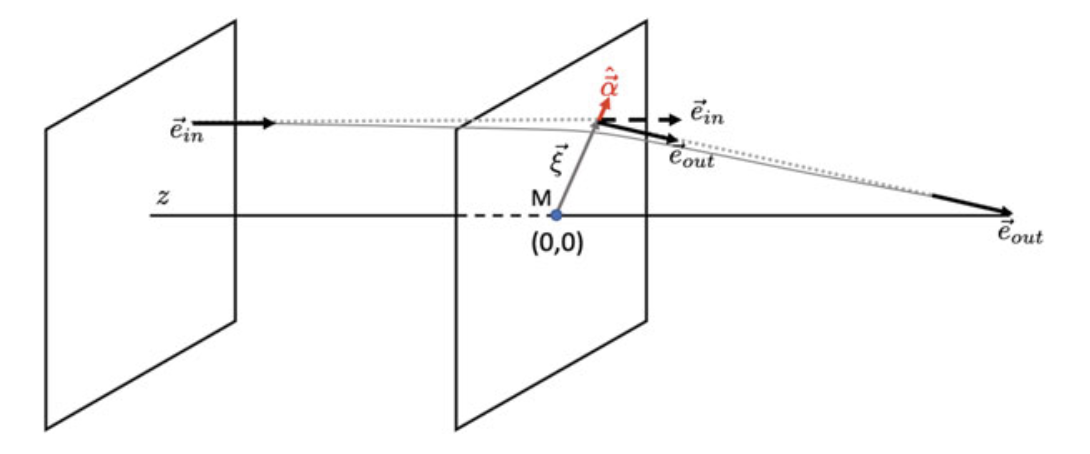
\includegraphics[width=\linewidth, keepaspectratio]{img//chapter2/bornapprox.png}
    \caption[Born approximation schematics]{Schematics for the Born approximation.\\\small{Credits: \cite{meneghetti_introduction_2021}.}}
    \label{fig:bornapprox}
\end{figure}

If the lens can be approximated by a point mass, the potential is $\f = -\frac{G M}{\sqrt{\x^2 + z^2}}$, where $G$ is the gravitational constant, and thus \cref{eq:2.4} simplifies to the following:
\be
\label{eq:2.5}
\hat{\va{\a}} (\va{\x}) = \frac{4 G M}{c^2 \x} \vec{e}_\x = \frac{4 G M}{c^2 \x^2} \va{\x} \;.
\ee

Under the assumption of weak field, the superposition principle can be applied to extend the previous definition to calculate the deflection angle of an ensemble of point-like lenses. Having a sparse distribution of $N$ point masses on a plane, the deflection angle of a light ray crossing the plane at $\va{\x}$ will be
\be
\label{eq:2.6}
\hat{\va{\a}} (\va{\x}) = \sum_i^N \hat{\va{\a}}_i (\va{\x} - \va{\x}_i) = \frac{4 G}{c^2} \sum_i^N M_i \frac{\va{\x} - \va{\x}_i}{{|\va{\x} - \va{\x}_i|}^2} \,,
\ee
where $\va{\x}_i$ and $M_i$ are the positions and masses of each lens.

When discussing more realistic situations of lensing, such as those involving three-dimensional distributions of matter, it is important to note that the physical extent of the lens is typically much smaller than the distances between the observer, the lens, and the source. Consequently, the bending of light occurs primarily over a brief segment of its path. This observation allows for the application of the \emph{thin screen approximation}, where the lens is represented as a planar distribution of matter, termed the lens plane. In this simplified model, the distribution of matter responsible for lensing is completely characterized by its surface density
\be
\label{eq:2.7}
\S (\va{\x}) = \int \r (\va{\x}, z) \dd{z} \,,
\ee
where $\va{\x}$ is a two-dimensional vector on the lens plane and $\r$ is the three-dimensional density.

In this context, the total deflection angle can be obtained by summing the contributions of all the mass elements $\S (\va{\x}) \dd^2{\x}$:
\be
\label{eq:2.8}
\hat{\va{\a}} (\va{\x}) = \frac{4 G}{c^2} \int \frac{(\va{\x} - \va{\x}^\prime) \S (\va{\x}^\prime)}{{|\va{\x} - \va{\x}^\prime|}^2} \dd^2{\x^\prime} \,.
\ee

% *************************************************************
%%%%% SECTION 2.2: LENS EQUATION %%%%%
\section{Lens equation}
\label{sec:lens_equation}

In order to define the observable light path, the connection between the observed and true positions of a source during a gravitational lensing event must be explored. Without the presence of the lens, light from a distant source would travel directly to an observer who would perceive the source at a specific location in the sky, denoted by $\va{\b}$ (measured in angular units), representing the source's \emph{intrinsic} position. However, when the gravitational lens causes a deflection of the photons, the observer detects them coming from an altered direction $\va{\t}$, which is known as the \emph{apparent} (or \emph{observed}) \emph{image} position of the source.

Following the typical gravitational lensing geometry, depicted in \cref{fig:lensing_sketch}, a mass is placed at redshift $z_L$, which equates to an angular diameter distance $D_L$. This mass acts as a lens, deflecting light rays coming from a source located at redshift $z_S$ (corresponding to an angular distance $D_S$). An observer at $z_O=0$ gathers the photons originating from this distant source. The angular diameter distance from the lens to the source is denoted as $D_{LS}$.

\begin{figure}
    \centering
    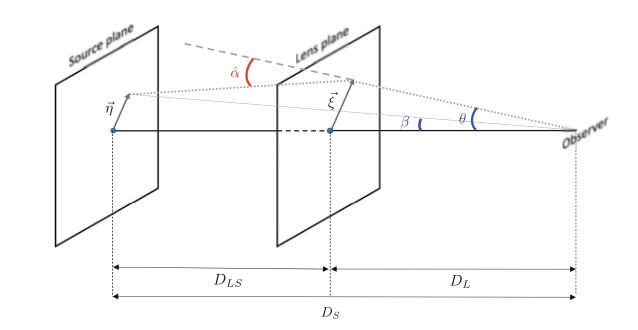
\includegraphics[width=\linewidth, keepaspectratio]{img/chapter2/lensing_sketch.png}
    \caption[Lensing system geometry]{Typical lensing system geometry.\\\small{Credits: \cite{meneghetti_introduction_2021}.}}
    \label{fig:lensing_sketch}
\end{figure}

A source located at the intrinsic angular position $\va{\b}$, which lies on the source plane at a distance $\va{\h} = \va{\b} D_S$ from the optical axis, emits photons that pass through the lens plane at a point $\va{\x} = \va{\t} D_L$. These photons are then deflected by an angle $\hat{\va{\a}}$, ultimately reaching the observer. The magnitude of this deflection is specified by \cref{eq:2.4}.
As a result of this deflection, the observer perceives the light as originating from the apparent angular position $\va{\t}$.

When the angles $\va{\t}$, $\va{\b}$, $\hat{\va{\a}}$ are small, the actual position of the source and where it appears to be located in the sky are connected by a straightforward relationship, the so-called \emph{lens equation}:
\be
\label{eq:2.9}
\va{\t} D_S = \va{\b} D_S + \hat{\va{\a}} D_{LS} \,.
\ee

Defining then the reduced deflection angle as
\be
\label{eq:2.10}
\va{\a} (\va{\t}) \equiv \dfrac{D_{LS}}{D_S} \hat{\va{\a}} (\va{\t}) \,,
\ee
\cref{eq:2.9} can be rewritten as
\be
\label{eq:2.11}
\va{\b} = \va{\t} - \va{\a} (\va{\t}) \,,
\ee
which allows to determine the intrinsic source position if the image position and the deflection angle are known. In contrast, by solving the lens equation for the unknown $\va{\t}$, it is possible to compute the image position(s) of a source placed at $\va{\b}$, lensed by a lens with a deflection field $\va{\a} (\va{\t})$.

A common choice is to write the lens equation in its dimensionless form by defining a length scale $\x_0$ on the lens plane and a corresponding length scale $\h_0 = \x_0 D_S / D_L$ on the source plane and using them to define the dimensionless (scaled) vectors
\be
\label{eq:2.12}
\vec{x} \equiv \frac{\va{\x}}{\x_0} \;,\quad \vec{y} \equiv \frac{\va{\h}}{\h_0} \,,
\ee
as well as the dimensionless deflection angle
\be
\label{eq:2.13}
\va{\a} \bp{\vec{x}} = \frac{D_L D_{LS}}{\x_0 D_S} \hat{\va{\a}} \bp{\x_0 \vec{x}} \,.
\ee

By substituting these dimensionless quantities into \cref{eq:2.11}, the dimensionless lens equation can be obtained
\be
\label{eq:2.14}
\vec{y} = \vec{x} - \va{\a} (\vec{x}) \,.
\ee


%%%%%%%%%%%%%%%%%%%%%%%%%%%%%%%%%%%%%%%%%%%%%%%%%%%%%%%
%%%%% Lensing potential and convergence %%%%%
%%%%%%%%%%%%%%%%%%%%%%%%%%%%%%%%%%%%%%%%%%%%%%%%%%%%%%%
\subsection{Lensing potential and convergence}
\label{subsec:lensing_potential_convergence}
The deflection properties of an extended distribution of matter are defined by its \emph{effective lensing potential}, namely the properly re-scaled projection on the lens plane of the three-dimensional Newtonian potential $\F$:
\be
\label{eq:2.15}
\hat{\P} (\va{\t}) = \frac{2}{c^2} \frac{D_{LS}}{D_L D_S} \int \F (D_L \va{\t}, z) \dd{z} \,.
\ee

It can be shown that the effective lensing potential satisfies two important properties:
\begin{enumerate}
    \item the gradient of $\hat{\P}$ is the reduced deflection angle:
    \be
    \label{eq:2.16}
    \va{\nabla}_\t \hat{\P} (\va{\t}) = \va{\a} (\va{\t}) \,;
    \ee

    \item the Laplacian of $\hat{\P}$ is twice the \emph{convergence} $\k$:
    \be
    \label{eq:2.17}
    \laplacian_\t \hat{\P} (\va{\t}) = 2 \k (\va{\t}) \,.
    \ee
\end{enumerate}

The convergence is defined as a dimensionless surface density
\be
\label{eq:2.18}
\k (\va{\t}) \equiv \frac{\S (\va{\t})}{\S_{cr}} \quad \mathrm{with} \quad \S_{cr} = \frac{c^2}{4 \pi G} \frac{D_S}{D_L D_{LS}} \;,
\ee
where $\S_{cr}$ is the so-called \emph{critical surface density}, a pivotal characteristic of the lens system, a function of the angular diameter distances of the lens and source, which allows to discriminate between \emph{strong} and \emph{weak} gravitational lensing regimes.

In particular, strong lensing is usually observed in regions of high mass concentration, such as the cores of galaxy clusters or around massive galaxies, when the surface mass density of the lens is comparable to or exceeds the critical surface density ($\S \geq \S_{cr}$) and the gravitational field of the lens is strong enough to produce multiple images of the source, form Einstein rings, or create arc-like structures.
On the contrary, weak lensing occurs when the surface mass density of the lens is below the critical surface density ($\S < \S_{cr}$). The gravitational effect is subtler, leading to slight distortions in the shapes of background galaxies, which can only be detected statistically over large populations of galaxies. Weak lensing does not produce multiple images or highly visible arcs but instead slightly stretches the images of background galaxies, causing shear and magnification effects.

From the previous definitions in \cref{eq:2.15,eq:2.18}, lensing quantities such as lensing potential (and therefore deflection angle) and critical surface density strongly depend on distances between observer, lens and source, which in turn depend on the source and lens redshifts.
The distance ratio
\be
\frac{D_L D_{LS}}{D_S}
\ee
is called \emph{lensing distance} and \cref{fig:lensing_distance} shows how it varies with the redshifts of source and lens.
As can be seen, the lensing distance increases with the source redshift and peaks when the lens is at an intermediate distance between the source and the observer. Clearly, the larger the lensing distance (and so the convergence), the stronger the effects generated by the lensing event.

\begin{figure}
  \centering
  \subfloat[]{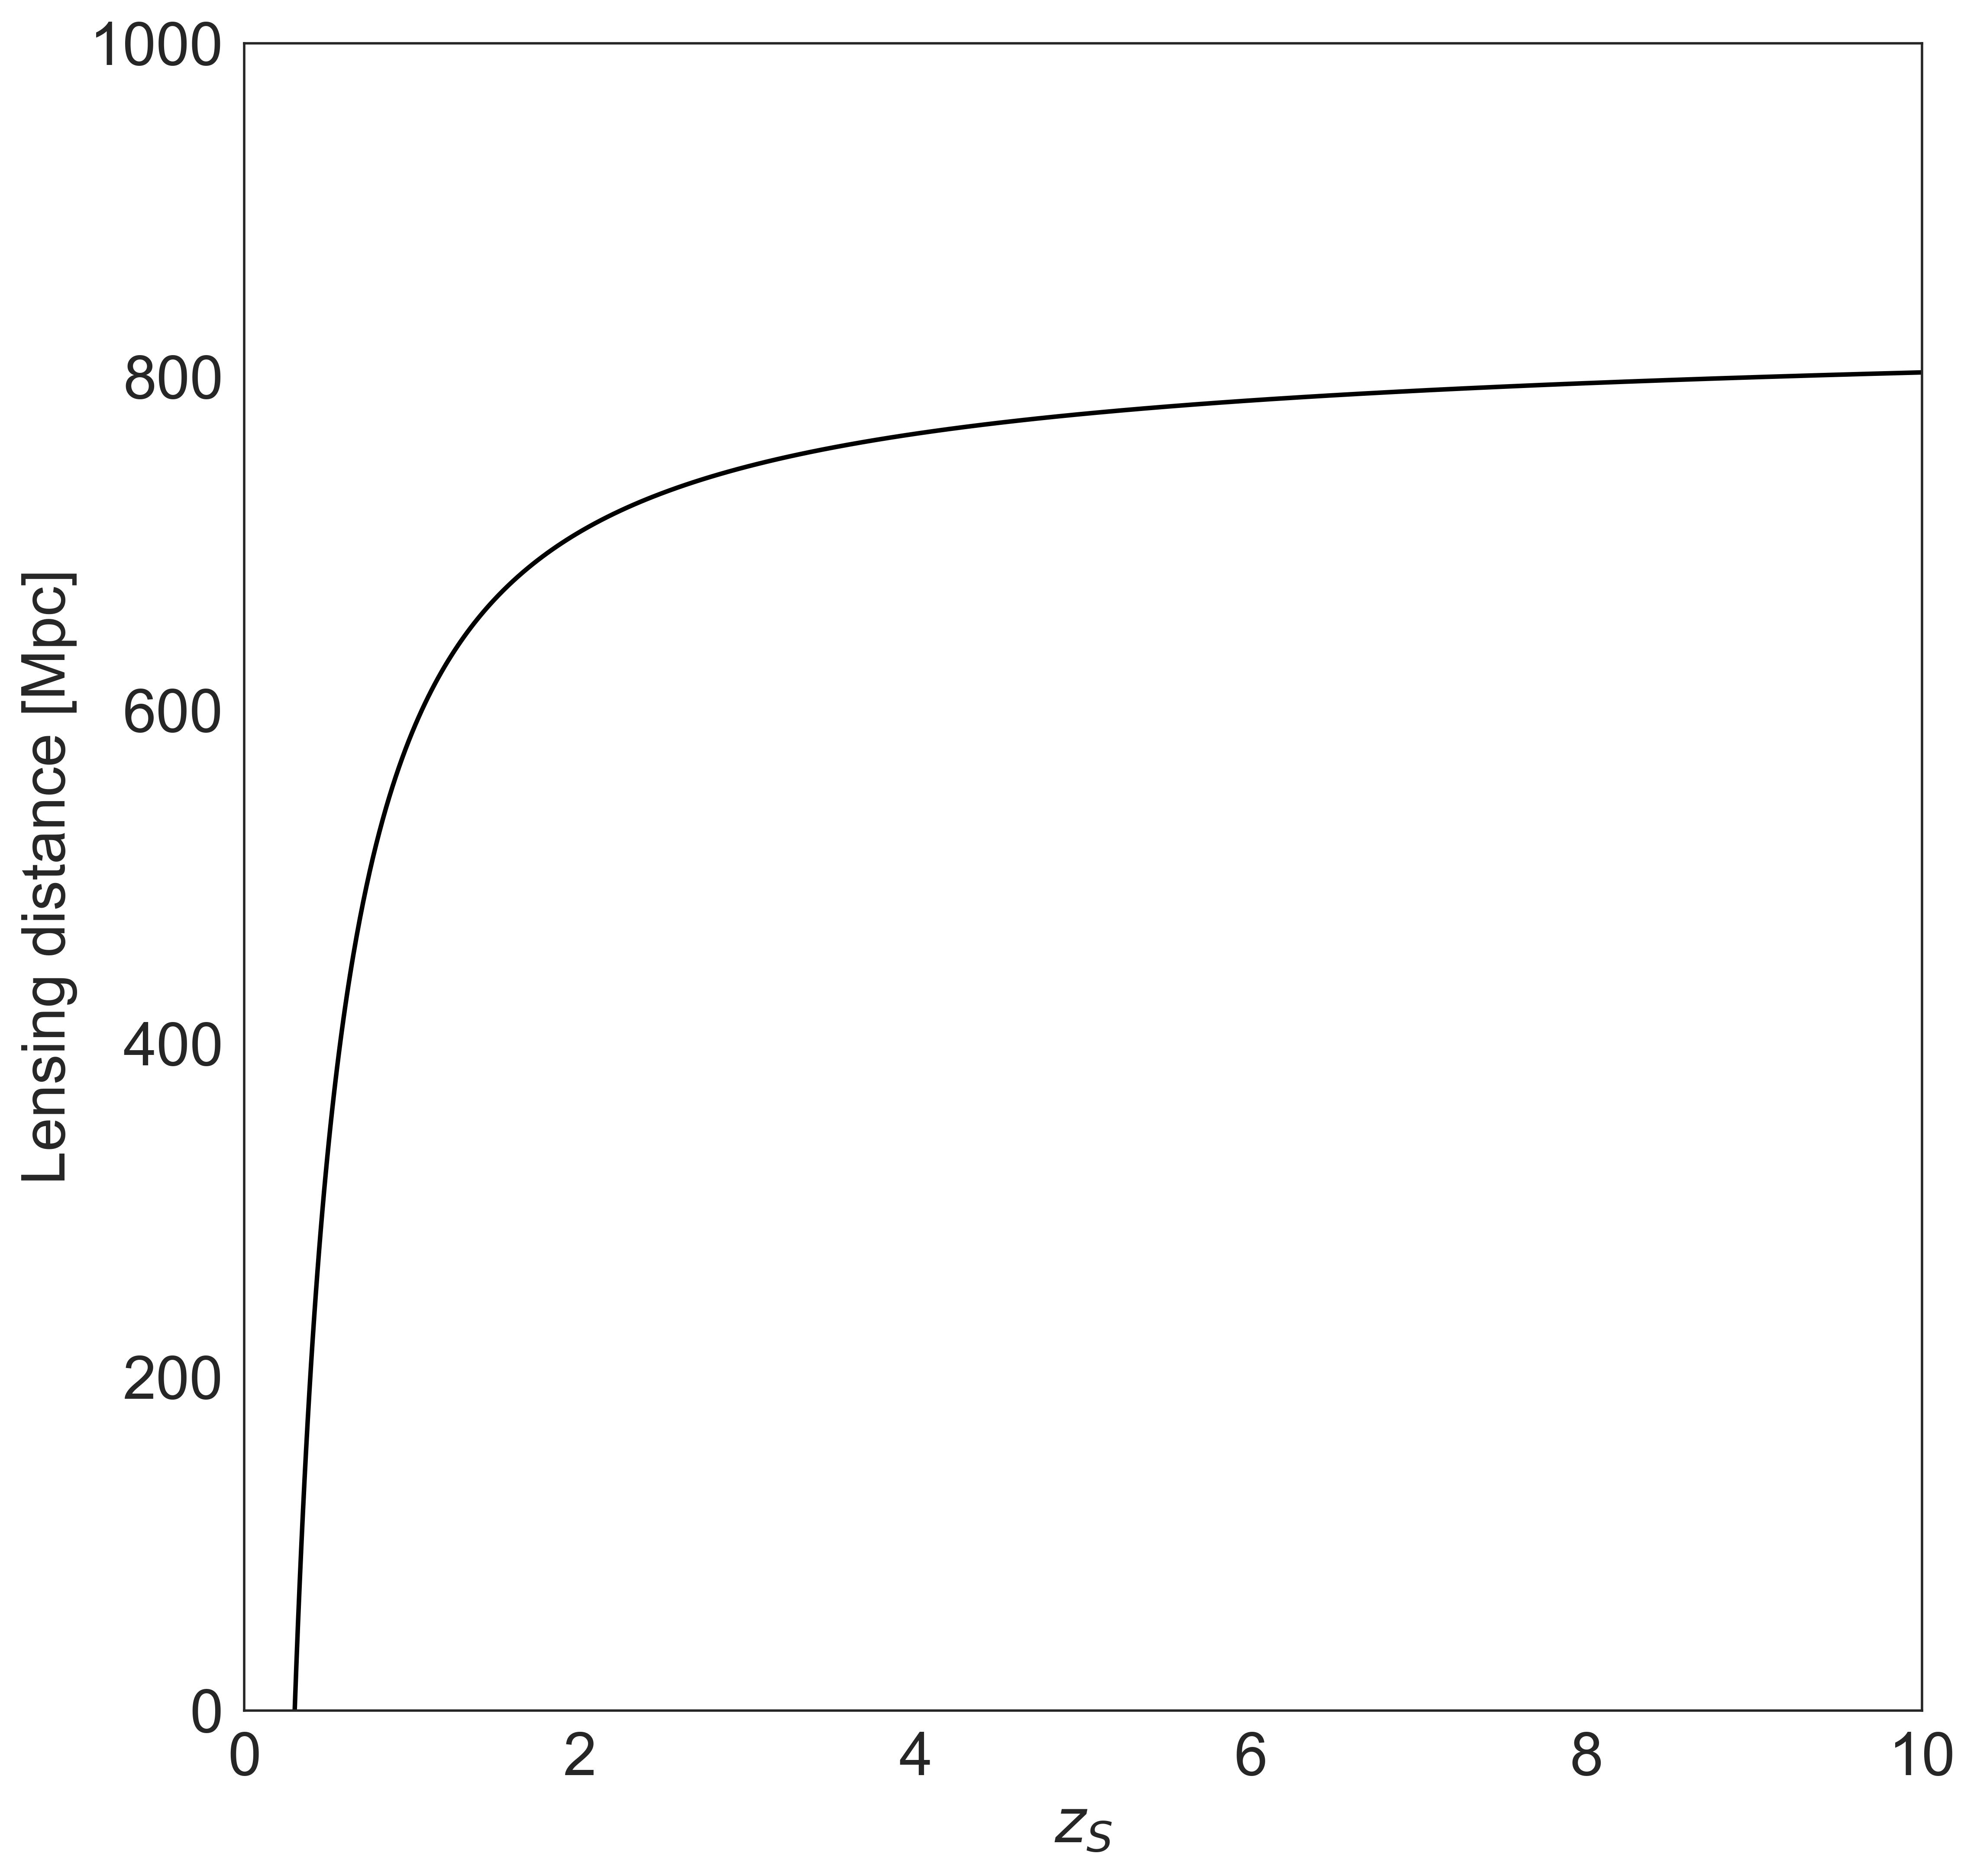
\includegraphics[width=0.5\linewidth, keepaspectratio]{img/chapter2/lensing_distance_a.png}\label{fig:lensing_distance_a}}
  \hfill
  \subfloat[]{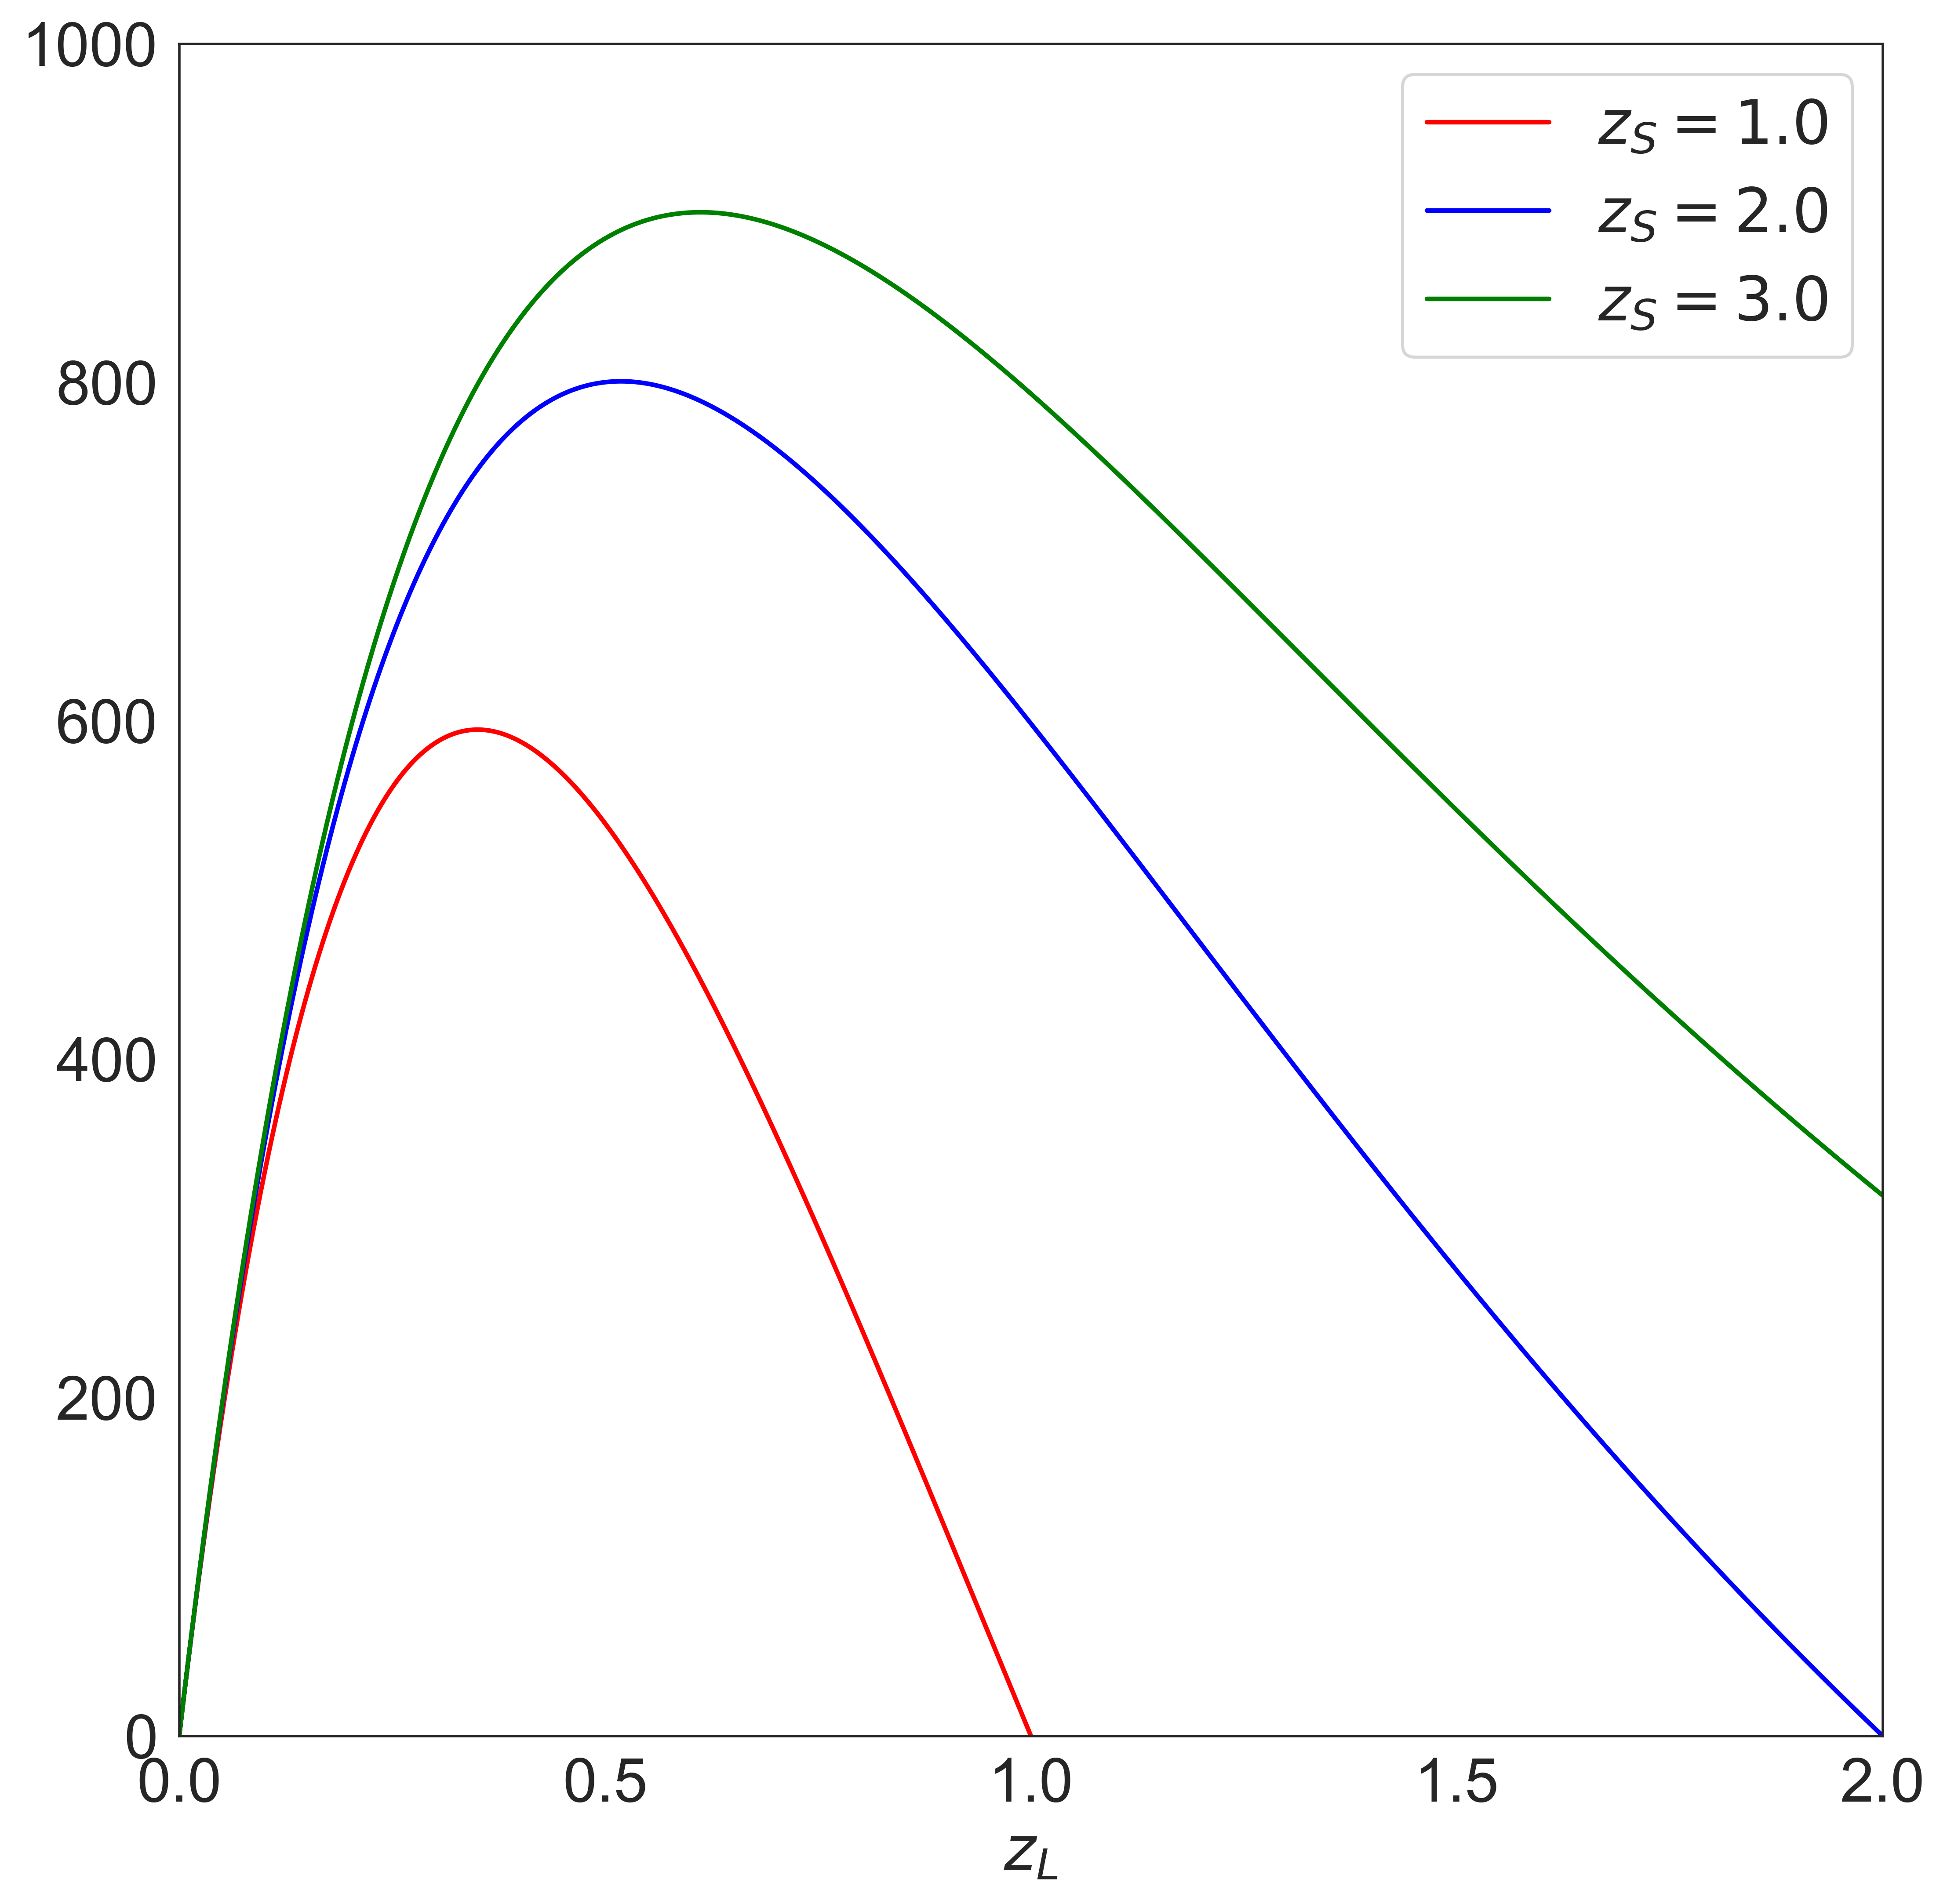
\includegraphics[width=0.5\linewidth, keepaspectratio]{img/chapter2/lensing_distance_b.png}\label{fig:lensing_distance_b}}
  \caption[Lensing distance variation with redshifts]{\protect\subref{fig:lensing_distance_a} Lensing distance variation as a function of the source redshift and \protect\subref{fig:lensing_distance_b} as a function of the lens redshift.}
  \label{fig:lensing_distance}
\end{figure}


%%%%%%%%%%%%%%%%%%%%%%%%%%%%%%%%%%%%%%%%%%%%%%%%%%%%%%%
%%%%% First-order lens mapping %%%%%
%%%%%%%%%%%%%%%%%%%%%%%%%%%%%%%%%%%%%%%%%%%%%%%%%%%%%%%
\subsection{First-order lens mapping}
\label{subsec:first_order_mapping}
A significant effect of gravitational lensing is image distortion. This alteration becomes markedly noticeable with sources of extended size. For instance, galaxies in the background can be observed as elongated arcs when they are lensed by clusters of galaxies or individual galaxies. The cause of this distortion is the varying deflection of light rays. Ideally, by solving the lens equation for every point of the extended source, the configuration of the images can be determined. Specifically, when the size of the source is significantly less than the angular scale over which the lens deflection angle field varies, the correspondence between the position of the source and the images can be approximated as linear on a local scale, allowing for a first-order approximation.

By computing the distance between two points $\va{\b}$ and $\va{\b}^\prime = \va{\b} + \dd{\va{\b}}$ on the source plane, it is possible to define a linear mapping between the source and the lens plane, described by the Jacobian matrix
\be
\label{eq:2.19}
A \equiv \frac{\partial \va{\b}}{\partial \va{\t}} = \bp{\d_{ij} - \frac{\partial \a_i (\va{\t})}{\partial \t_i}} = \bp{\d_{ij} - \frac{\partial^2 \hat{\P} (\va{\t})}{\partial \t_i \partial \t_j}} \,.
\ee

This metric is a second-rank symmetric tensor called the \emph{lensing Jacobian} and can be divided into an isotropic and an anisotropic part:
\begin{subequations}
\begin{align}
    \label{eq:2.20a}
    A_{iso, ij} & = \frac{1}{2} \Tr A \d_{ij} = \bp{1 - \frac{1}{2} \laplacian \hat{\P}} \d_{ij} = \bp{1 - \k} \d_{ij} \,,
    \\
    \label{eq:2.20b}
    A_{aniso, ij} & = A_{ij} - \frac{1}{2} \Tr A \d_{ij} = \begin{pmatrix} -\frac{1}{2} \bp{\hat{\P}_{11} - \hat{\P}_{22}} & - \hat{\P}_{12} \\ - \hat{\P}_{12} & \frac{1}{2} \bp{\hat{\P}_{11} - \hat{\P}_{22}} \end{pmatrix} \,.
\end{align}
\end{subequations}

It is possible to describe the anisotropic component of the lensing Jacobian by defining the \emph{shear} tensor $\G$, a 2x2 symmetric, traceless tensor, usually written in the form of a pseudo-vector $\va{\g} = (\g_1, \g_2)$, whose components are:
\begin{subequations}
\begin{align}
    \label{eq:2.21a}
    \g_1 & = \frac{1}{2} \bp{\hat{\P}_{11} - \hat{\P}_{22}}  \,,
    \\
    \label{eq:2.21b}
    \g_2 & = \hat{\P}_{12} = \hat{\P}_{21} \,.
\end{align}
\end{subequations}

The shear tensor has eigenvalues $\pm \sqrt{\g_1^2 + \g_2^2} = \pm \g$ and, representing the direction of the eigenvector corresponding to the positive eigenvalue with $\f$, $\G$ can be written as:
\be
\label{eq:2.22}
\G = \begin{pmatrix} \g_1 & \g_2 \\ \g_2 & - \g_1 \end{pmatrix} = \g \begin{pmatrix} \cos{2\f} & \sin{2\f} \\ \sin{2\f} & - \cos{2\f} \end{pmatrix} \,.
\ee

Summarizing, from \cref{eq:2.20a,eq:2.20b} and considering this last definition of $\G$, the lensing Jacobian becomes
\be
\label{eq:2.23}
A = (1 - \k) 
    \begin{pmatrix} 1 & 0 \\ 0 & 1 \end{pmatrix} - \g \begin{pmatrix} \cos{2\f} & \sin{2\f} \\ \sin{2\f} & - \cos{2\f} \end{pmatrix} = \begin{pmatrix} 1 - \k - \g_1  & - \g_2 \\ - \g_2 & 1 - \k + \g_1 \end{pmatrix} \,.
\ee

From the last expression of the lensing Jacobian, it can be seen that the first-order mapping is characterized by two parts. The first term, depending on the convergence, describes an isotropic transformation of the source image, which is therefore expanded or contracted by the same factor in all directions.
Instead, the second term describes an anisotropic transformation dependent on the shear, and thus causes distortions of the source image along a specific direction, given by the angle $\f$. More precisely, the image size is increased compared to the source in the direction of the eigenvectors of $A$ with eigenvalue $\g$, and decreased in the perpendicular direction. The amounts of these magnifications and de-magnifications are given by the inverse of the tangential and radial eigenvalues, namely $\l_t = 1 - \k - \g$ and $\l_r = 1 - \k + \g$.

\begin{figure}
    \centering
    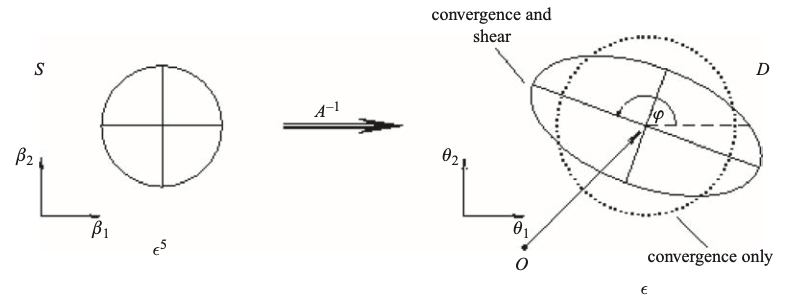
\includegraphics[width=\linewidth, keepaspectratio]{img//chapter2/convergence_shear.png}
    \caption[Convergence and shear distortion on circular source]{Distortion effects due to convergence and shear on a circular source.\\\small{Credits: \cite{mediavilla_lensing_2016}.}}
    \label{fig:convergence_shear}
\end{figure}

As an example, \cref{fig:convergence_shear} shows how a circular source of radius $r$ would be distorted by convergence and shear effects. Due to the convergence term, the source is mapped to a larger (or smaller) circle, whose radius is $r / (1 - \k)$.\\Due to the shear term, the circle is further elongated in the direction given by the angle $\f$ and contracted in the perpendicular direction to form an ellipse. 

\begin{figure}
    \centering
    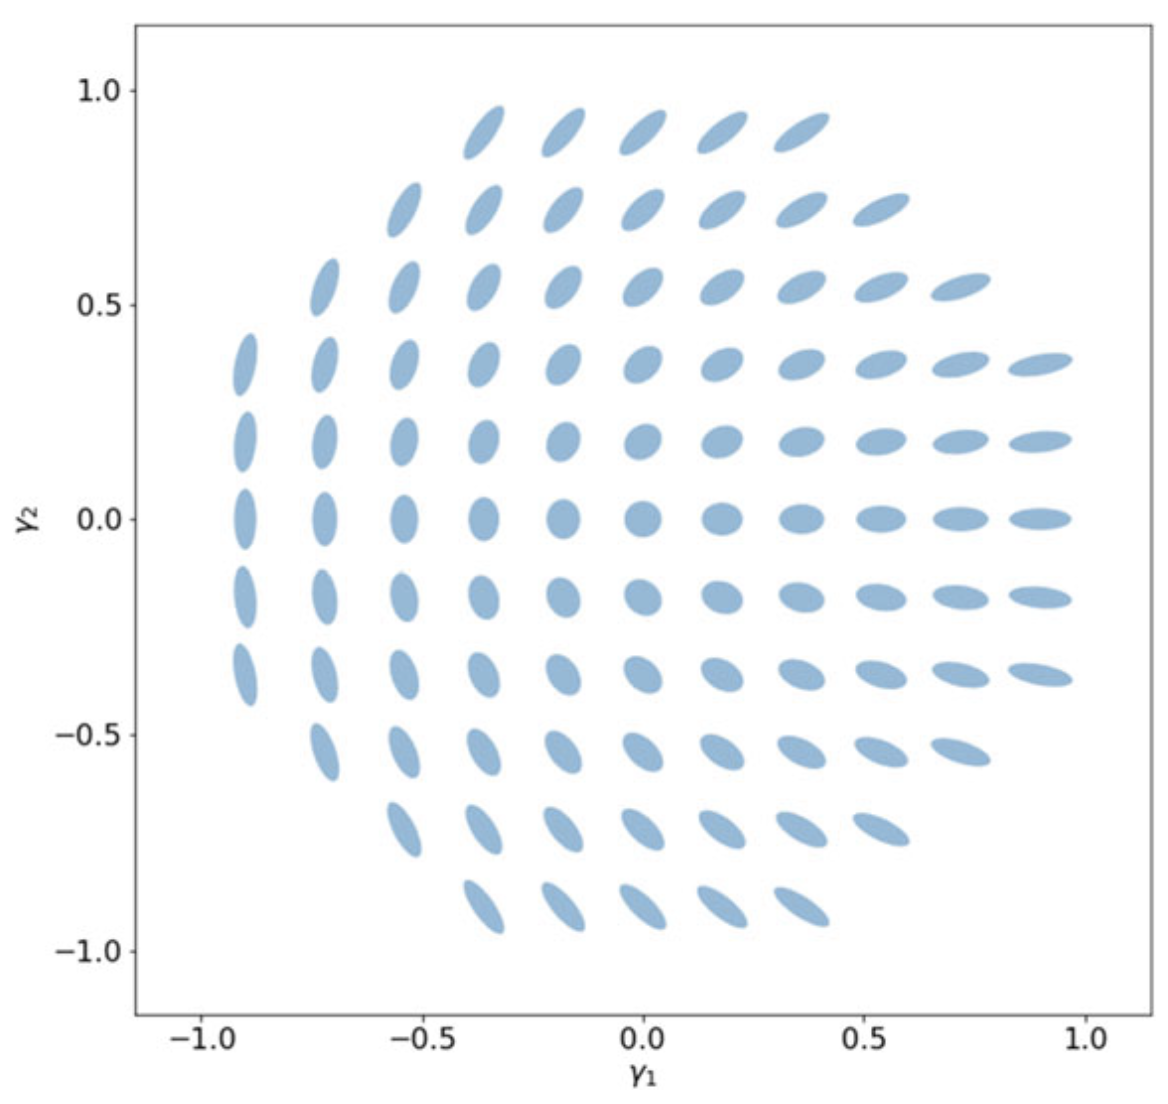
\includegraphics[width=0.7\linewidth]{img//chapter2/shear_orientations.png}
    \caption[Images orientations according to different combinations of $\g_1$ and $\g_2$]{Images orientations according to different combinations of $\g_1$ and $\g_2$.\\\small{Credits: \cite{meneghetti_introduction_2021}}.}
    \label{fig:shear_orient}
\end{figure}

This effect can be understood considering the circular source isophotes, described by
\be
\label{eq:source_isoph}
\b_1^2 + \b_2^2 = r^2 \,.
\ee

It is always possible to choose a reference frame where the Jacobian matrix is diagonal, so that the lens equation for a circular source is
\begin{subequations}
\begin{align}
    \label{eq:circu_lens1}
    \b_1 = (1 - \k - \g) \t_1 \,,
    \\
    \label{eq:circu_lens2}
    \b_2 = (1 - \k + \g) \t_2 \,.
\end{align}
\end{subequations}

By substituting these values into \cref{eq:source_isoph} the equation of the isophotes becomes
\be
\label{eq:ellipse_isoph}
(1 - \k - \g)^2 \t_1^2 + \b_2 = (1 - \k + \g)^2 \t_2^2 = r^2 \,,
\ee
which represents the equation for an ellipse, with major and minor axes $a = r/\l_t$ and $b = r/\l_r$, respectively.

Moreover, the fact that the shear tensor has spin 2 translates in different distortions according to its components:
\begin{itemize}
    \item $\g_1>0$, $\g_2 = 0$: major axis of the ellipse is along $\t_1$;
    \item $\g_1=0$, $\g_2 > 0$: major axis of the ellipse forms an angle of $\pi/4$ with $\t_1$;
    \item $\g_1<0$, $\g_2 = 0$: major axis of the ellipse is perpendicular to $\t_1$;
    \item $\g_1=0$, $\g_2 < 0$: major axis of the ellipse forms and angle of $3\pi/4$ with $\t_1$.
\end{itemize}

\Cref{fig:shear_orient} shows how images orientations are affected by these combinations of $\g_1$ and $\g_2$ and many more.


%%%%%%%%%%%%%%%%%%%%%%%%%%%%%%%%%%%%%%%%%%%%%%%%%%%%%%%
%%%%% Magnification %%%%%
%%%%%%%%%%%%%%%%%%%%%%%%%%%%%%%%%%%%%%%%%%%%%%%%%%%%%%%
\subsection{Magnification}
\label{subsec:magnification}
One of the most important features introduced by gravitational lensing is the \emph{magnification} effect: through the lens equation, the solid angle $\d \b^2$ is mapped to the solid angle $\d \t^2$. In the absence of photon emission or absorption, the Liouville theorem states that the surface brightness of a source remains constant as it passes through the lensing field. Thus, the change in the solid angle under which the source is observed implies that the flux received is magnified (or demagnified).
From \cref{eq:2.19}, the magnification introduced by the lensing is given by the inverse of the determinant of the Jacobian matrix. For this reason, the matrix $M = A^{-1}$ is called the \emph{magnification tensor} and therefore:
\be
\label{eq:2.24}
\m \equiv \det M = \frac{1}{\det A} = \frac{1}{(1- \k)^2 - \g^2} \,,
\ee
while the relation between intrinsic and observed flux can be written
\be
\label{eq:2.25}
F_\n = \int_I I_\n (\va{\t}) \dd^2{\t} = \int_S I_\n^S (\va{\b}(\va{\t})) \m (\va{\t}) \dd^2{\b} \,,
\ee
where the first integral is over the image plane and the second over the source plane.
From \cref{eq:2.24}, it is possible to define $\m_t = \l_t^{-1}$ and $\m_r = \l_r^{-1}$, the so-called \emph{tangential} and \emph{radial} magnification factors, so that $\m = \m_t \m_r$.

Since both convergence and shear (and therefore magnification) are functions of the position on the lens plane $\va{\t}$, there exists a set of critical points where $\det A = 0$, which means either $\l_t = 0$ or $\l_r = 0$. The ensemble of these points defines the \emph{critical lines}, along which the magnification diverges. By mapping the critical lines to the source plane through the lens equation, new sets of points are obtained, which are called \emph{caustics}.
The shape of these critical lines and caustics varies with the mass distribution of the lens. Some examples for different mass distributions are shown in \cref{fig:caustics_critlines}.

\begin{figure}
    \centering
    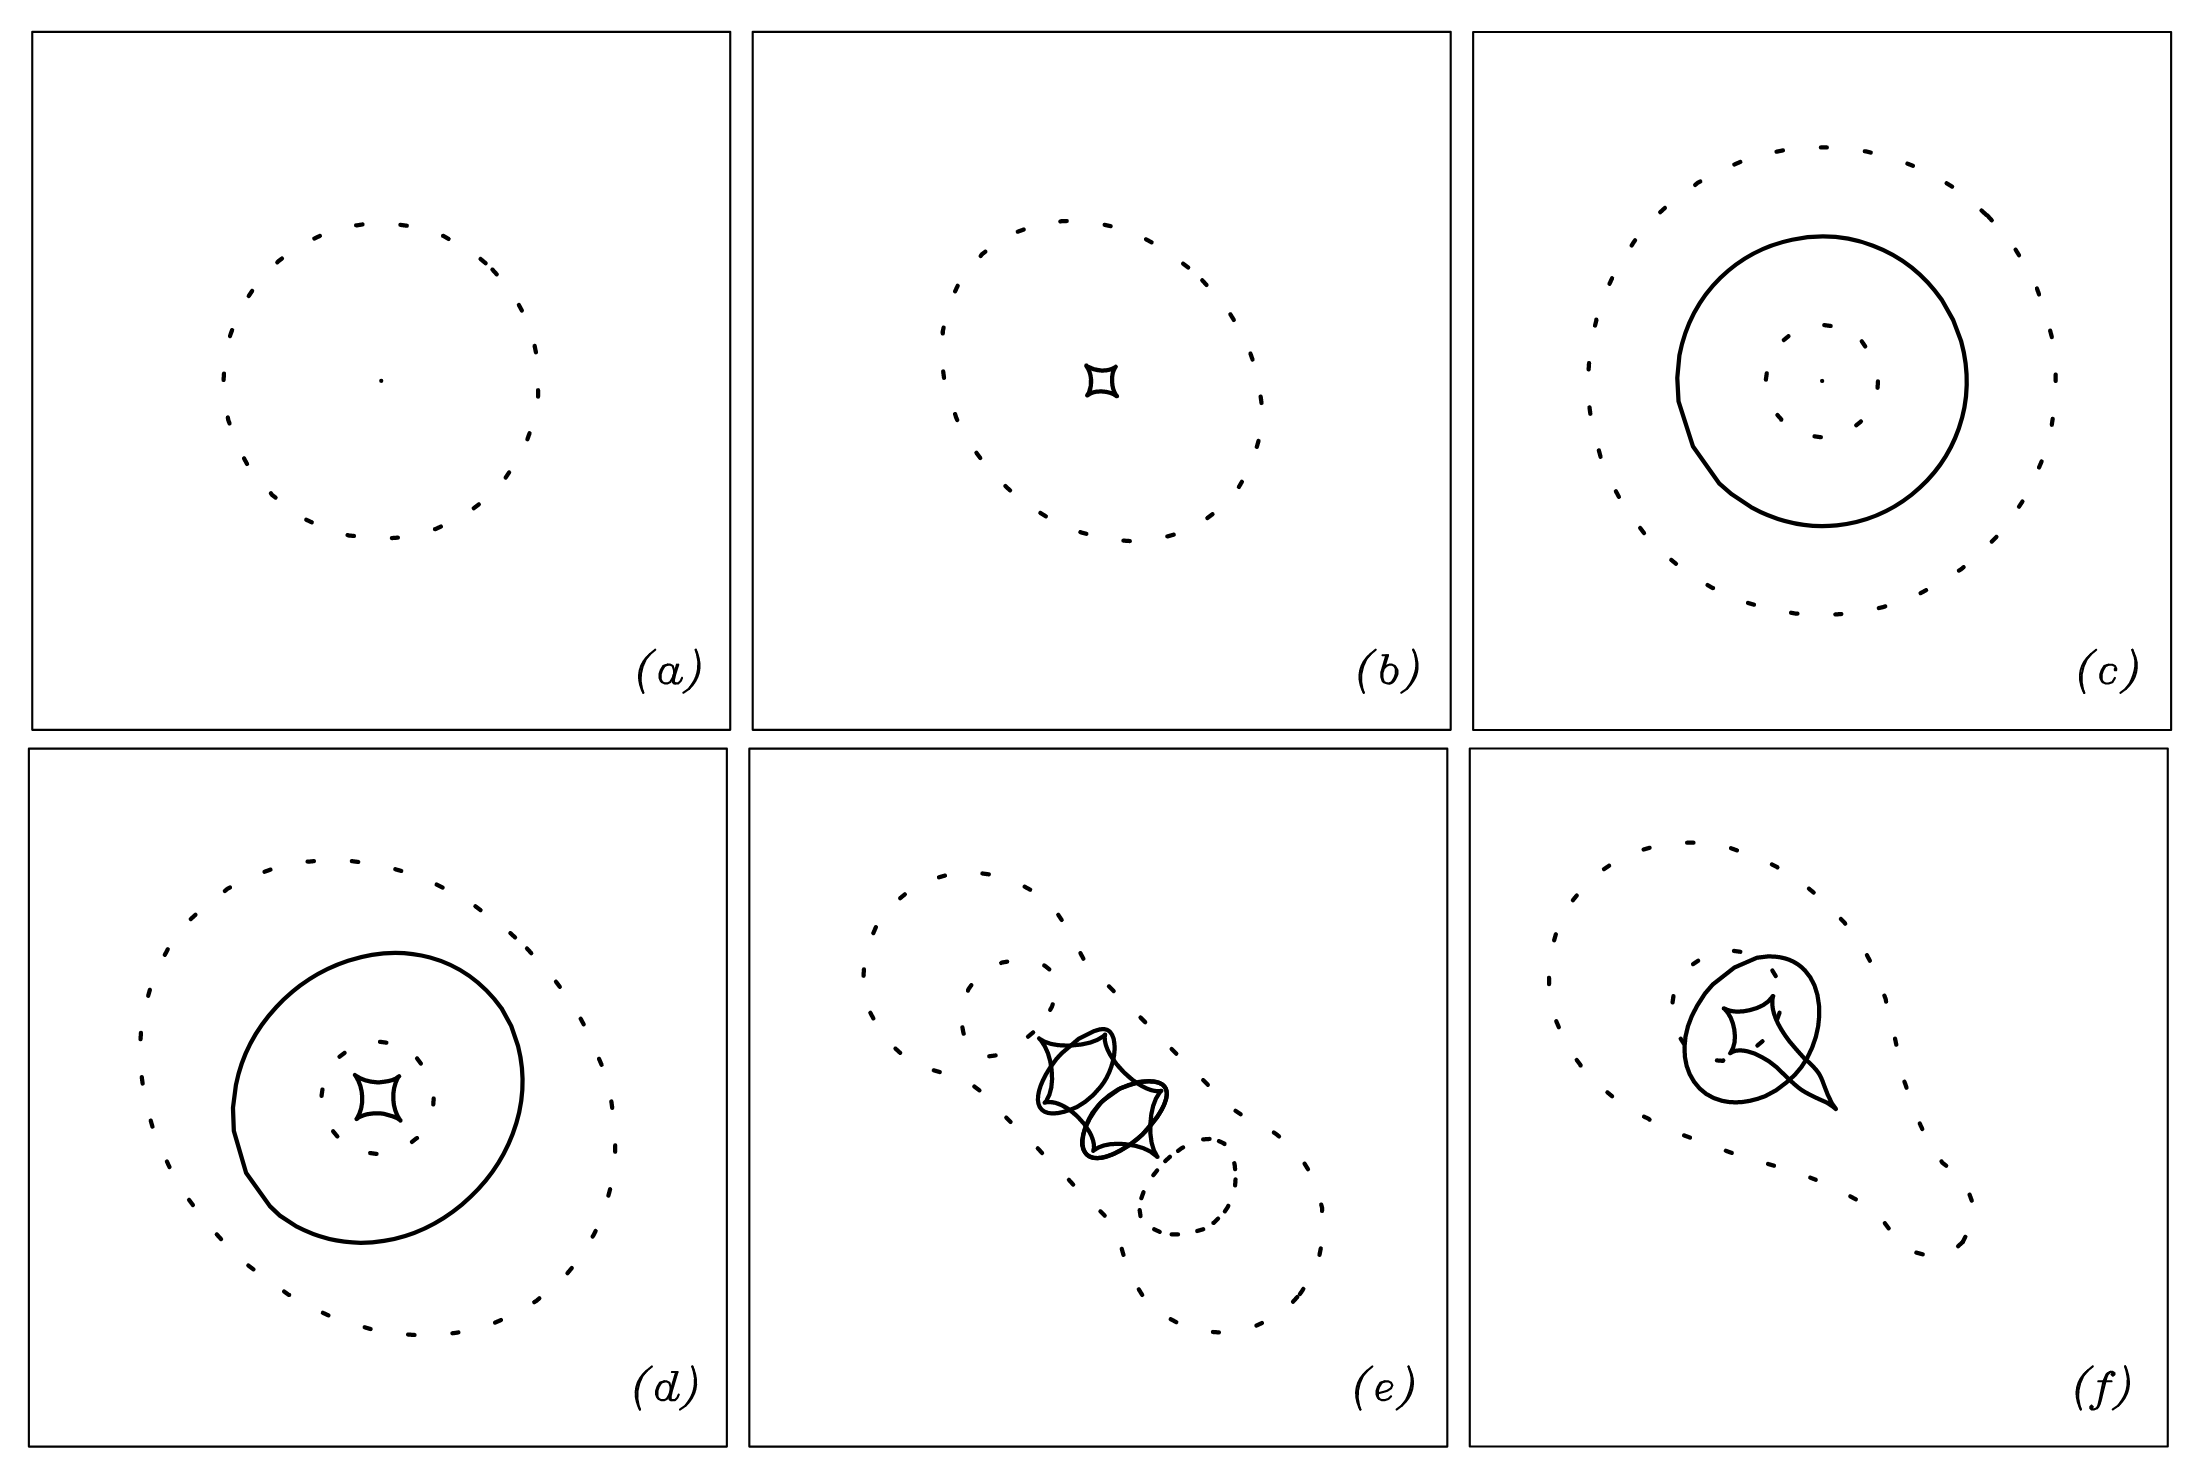
\includegraphics[width=0.6\linewidth, keepaspectratio]{img//chapter2/caustics_critlines.png}
    \caption[Caustics and critical lines shapes]{Caustics (solid) and critical lines (dashed) for different mass models: (a) a singular isothermal circular mass distribution generates only the critical lines, in particular the radial critical line is the central point and the tangential critical line is the circle; (b) a singular isothermal elliptical lens produces a tangential caustic (astroid) and the corresponding elliptical tangential critical line; (c) a circular and (d) elliptical mass distribution with shallower inner slope than the isothermal mass distribution generates both the critical lines and caustics; a bimodal mass distribution with two clumps of equal (e) or unequal (d) mass produces more complex critical lines and caustics.\\\small{Credits: \cite{kneib_cluster_2011}.}}
    \label{fig:caustics_critlines}
\end{figure}


%%%%%%%%%%%%%%%%%%%%%%%%%%%%%%%%%%%%%%%%%%%%%%%%%%%%%%%
%%%%% Time-delay and multiple images %%%%%
%%%%%%%%%%%%%%%%%%%%%%%%%%%%%%%%%%%%%%%%%%%%%%%%%%%%%%%
\subsection{Time-delay and multiple images}
\label{subsec:time_delay_images}
The deflection of light by a gravitational potential causes a delay in the travel time of light between the source and the observer, resulting in the appearance of multiple images of the source on the lens plane at different times.
This time delay has two components: one is geometrical, due to the different path length of the deflected light rays compared to the unperturbed ones, and one is gravitational, due to the effective speed of light in the presence of a gravitational potential.

The total time delay as a function of the position of the image, for a given source and lens, can be described by a surface known as \emph{time delay surface}:
\be
\label{eq:2.26}
t (\va{\t}) = t_{geom} + t_{grav} = \frac{(1 + z_L)}{c} \frac{D_L D_S}{D_{LS}} \left[ \frac{1}{2} (\va{\t} - \va{\b})^2 - \hat{\P} (\va{\t}) \right] = \frac{D_{\D t}}{c} \tau (\va{\t}) \,,
\ee
where $z_L$ is the lens redshift and the quantities
\begin{subequations}
\begin{align}
    \label{eq:2.27a}
    D_{\D t} & = (1 + z_L) \frac{D_L D_S}{D_{LS}} \,,
    \\
    \label{eq:2.27b}
    \tau (\va{\t}) & = \frac{1}{2} (\va{\t} - \va{\b})^2 - \hat{\P} (\va{\t})
\end{align}
\end{subequations}
are called \emph{time delay distance} and \emph{Fermat potential}, respectively.

The lens equation can be obtained taking the gradient of \cref{eq:2.26}:
\be
\label{eq:2.28}
\va{\nabla} \left[ \frac{1}{2} (\va{\t} - \va{\b})^2 - \hat{\P} (\va{\t}) \right] = 0 \,.
\ee

Therefore, the images are formed at the stationary points of the time delay surface, whose curvature is given by its Hessian matrix:
\be
\label{eq:2.29}
T_{ij} = \frac{\partial^2 t (\va{\t})}{\partial \t_i \partial \t_j} \propto (\d_{ij} - \hat{\P}_{ij}) = A_{ij} \,.
\ee

\begin{figure}[b!]
    \centering
    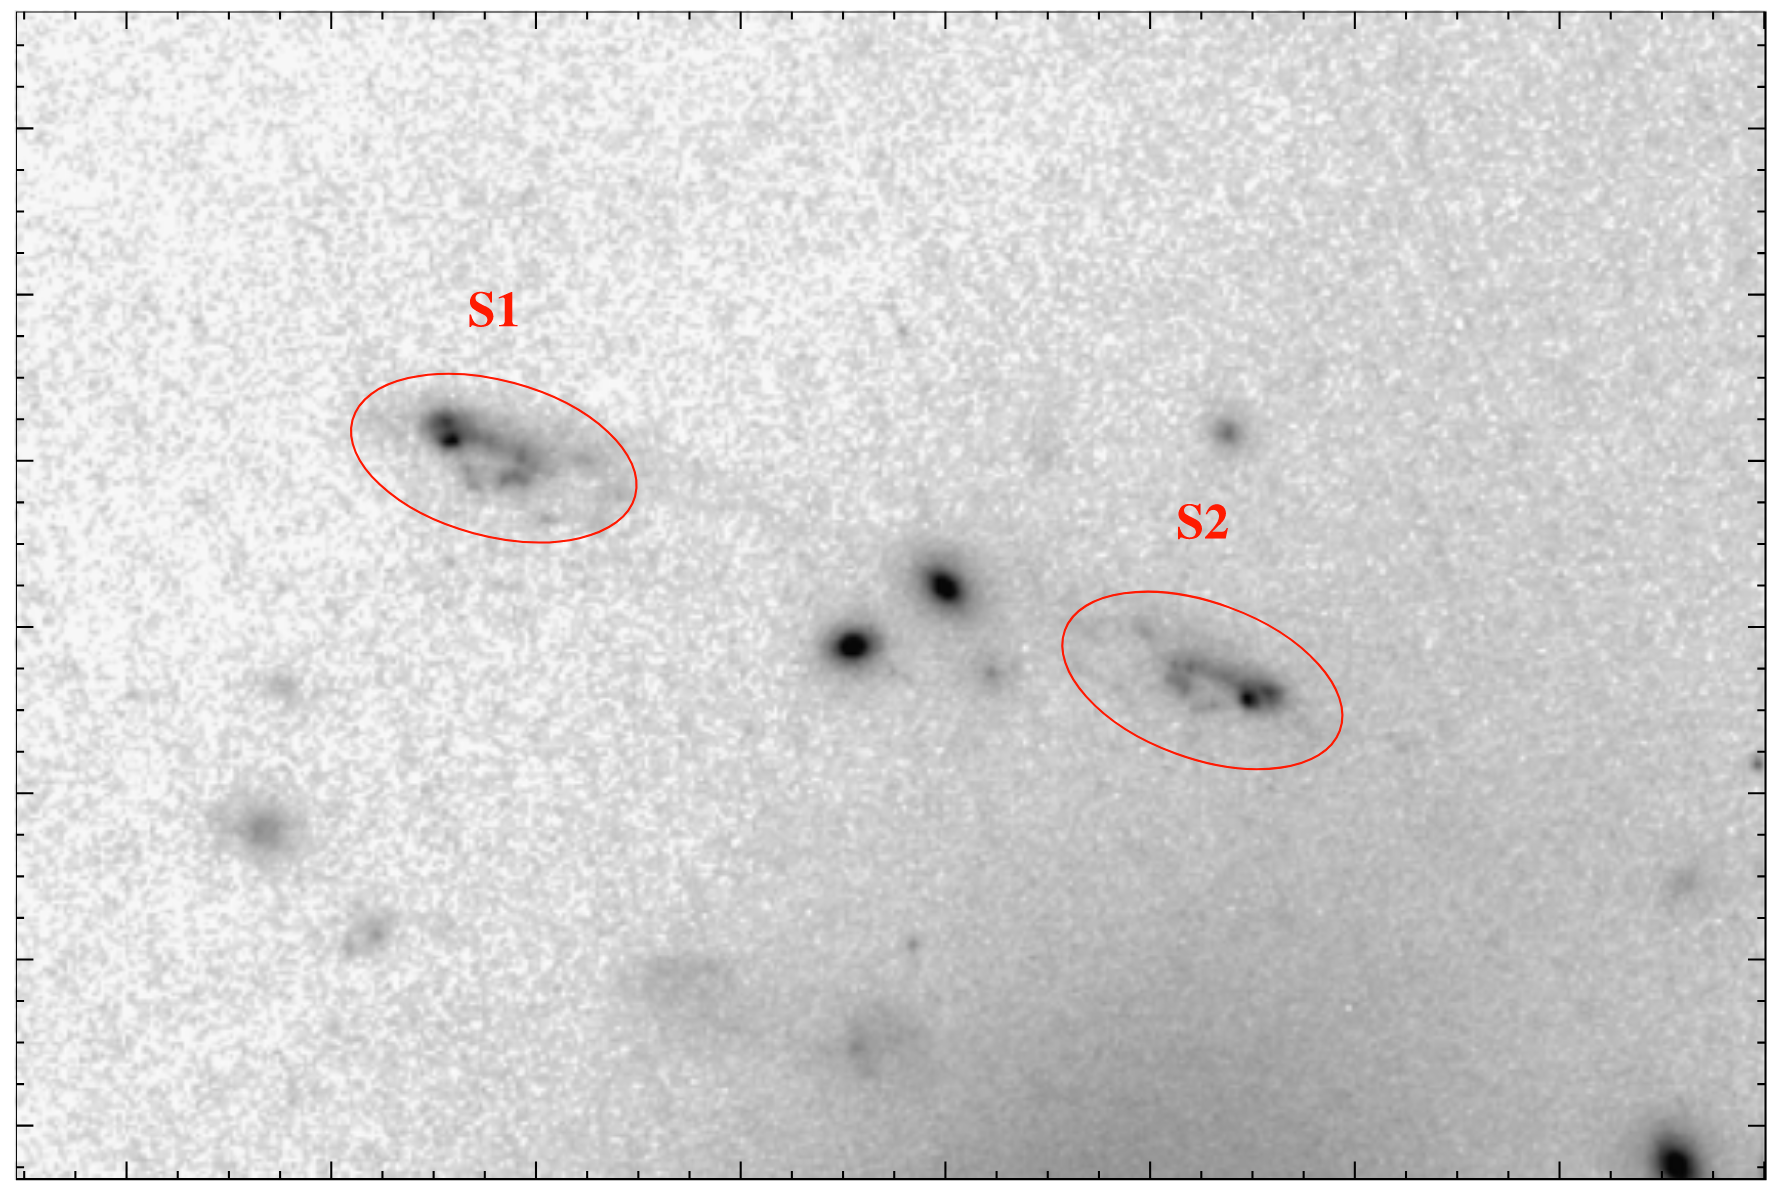
\includegraphics[width=0.9\linewidth, keepaspectratio]{img//chapter2/lensedpair.png}
    \caption[The lensed pair S1–S2 in AC114]{The lensed pair S1–S2 in AC114. This galaxy at $z = 1.867$ displays the surprising morphology of a hook, with an obvious change in parity.\\\small{Credits: \cite{kneib_cluster_2011}.}}
    \label{fig:lensedpair}
\end{figure}

The multiplicity of images in gravitational lensing is closely related to the characteristics of the time delay surface, and the configuration of this surface near stationary points offers insights into the shapes of the images and their \emph{parity}. Image parity is determined by the magnification sign: magnifications $>1$, whether positive or negative, both amplify the image. However, a positive magnification retains the original orientation of the unlensed source in the image, whereas a negative magnification results in an image with reversed parity.
Crossing a critical line results in a sign change in one of the Jacobian matrix's eigenvalues, leading to a shift in the image's parity. As a consequence, the parity of images located on opposite sides of a critical line is opposite to each other (\cref{fig:lensedpair}).
Furthermore, it can be shown that the number of images changes by two when the source crosses a caustic \citep{schneider_gravitational_1992} and that the total number of images of a generic lens is odd \citep{burke_multiple_1981}.

Different stationary points result in different types of image:
\begin{itemize}
    \item \textbf{type I images} arise at the minima of surface where both \cref{eq:2.29} eigenvalues are positive, so $\det A > 0 \,, \; \Tr A > 0$ $\rightarrow$ positive magnification;
    \item \textbf{type II images} appears at the saddle points of the surface where \cref{eq:2.29} eigenvalues have opposite signs, so $\det A < 0$ $\rightarrow$ negative magnification (\ie reversed image parity, not de-magnified);
    \item \textbf{type III images} arise at the maxima of the surface where both \cref{eq:2.29} eigenvalues are negative, so $\det A > 0 \,, \; \Tr A < 0$ $\rightarrow$ positive magnification.
\end{itemize}

\Cref{fig:timedelay1d} shows the geometrical and gravitational components of the time delay and their combination for a few positions of the source relative to the lens, considered axially symmetric. The geometric time delay is described by a parabola, and the gravitational function will vary depending on the potential considered.
In particular, for a source perfectly aligned with the center of the lens (top left of \cref{fig:timedelay3d}) there exist three stationary points, two of which (the minima) merge onto a single ring. This configuration is the so-called \emph{Einstein ring}. 

Thus, it is possible to introduce the so-called Einstein radius (\cref{fig:einsteinring}), which is properly an angle, useful to define the radius of the Einstein ring:
\be
\label{eq:2.30}
\t_E = \sqrt{\frac{4 G M(\t)}{c^2} \frac{D_{LS}}{D_L D_S}} \,.
\ee

\begin{figure}
  \centering
  \subfloat[]{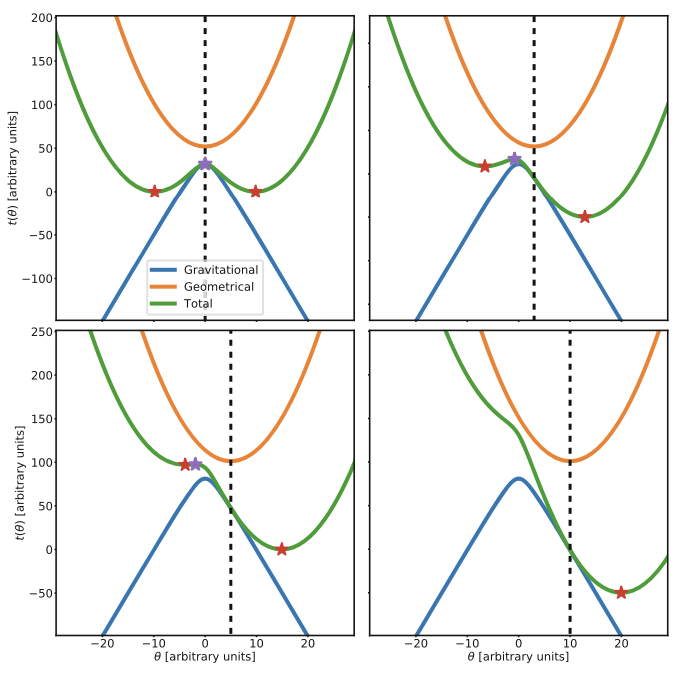
\includegraphics[width=0.5\linewidth, keepaspectratio]{img//chapter2/timedelay1d.png}\label{fig:timedelay1d}}
  \hfill
  \subfloat[]{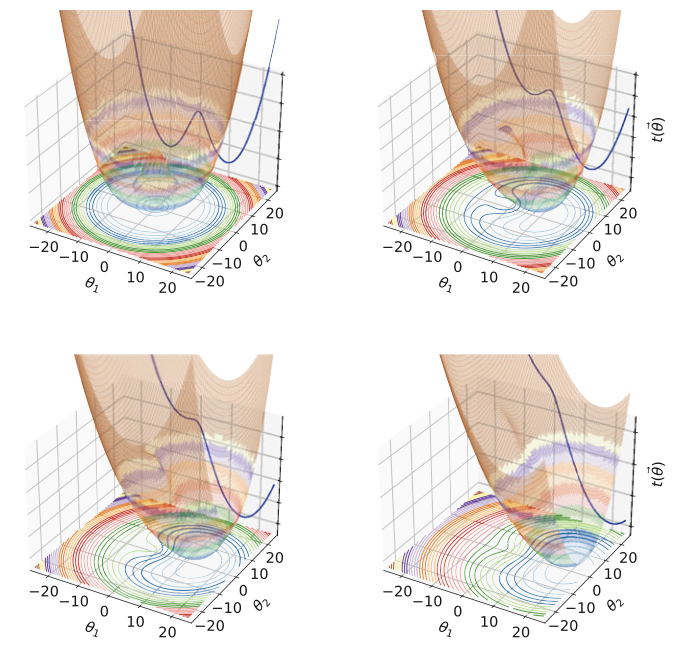
\includegraphics[width=0.5\linewidth, keepaspectratio]{img//chapter2/timedelay3d.png}\label{fig:timedelay3d}}
  \caption[Time delay functions and surfaces]{\protect\subref{fig:timedelay1d} One-dimensional time delay functions for a non-singular isothermal potential. The stars indicate the position of the images. Each panel corresponds to a different position of the source relative to the lens (dashed line). \protect\subref{fig:timedelay3d} Time delay surfaces for the same lens. Each panel corresponds to a different position of the source relative to the lens. Clearly visible Einstein ring in the top-left plot.\\\small{Credits: \cite{meneghetti_introduction_2021}.}}
  \label{fig:timedelay}
\end{figure}

\begin{figure}
    \centering
    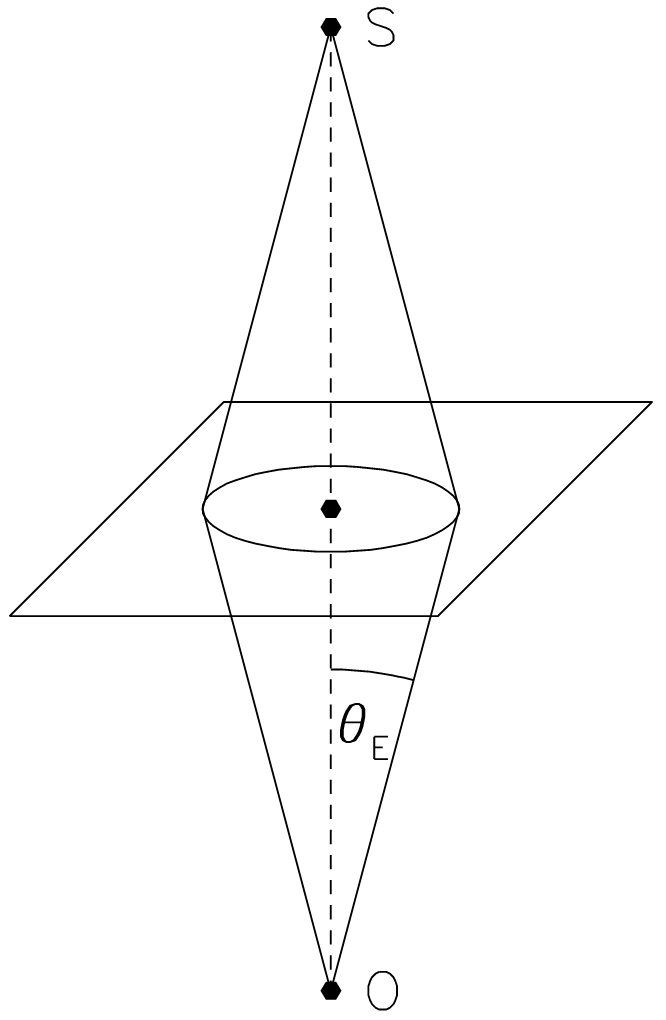
\includegraphics[width=0.22\linewidth, keepaspectratio]{img//chapter2/einsteinring.png}
    \caption[Einstein radius]{A source S exactly behind the center of an axially symmetric lens is mapped into the Einstein ring, with angular radius given by $\t_E$.\\\small{Credits: \cite{narayan_lectures_1997}.}}
    \label{fig:einsteinring}
\end{figure}


% *************************************************************
%%%%% CHAPTER 3: LENS MODELS %%%%%
\cleardoublepage
\chapter[Lens models]{Lens models}
\label{chap:lens_models}

This chapter delves into the intricate process of lens modeling, a pivotal technique for interpreting gravitational lensing observations. Gravitational lens models can be separated into two main categories: point-mass lenses (\ie \emph{microlenses}) and extended lenses, each possessing distinctive characteristics.
Microlensing refers to the lensing effect caused by objects with relatively small masses, such as stars or planets, acting as lenses. Unlike their more massive counterparts, microlenses do not produce multiple discernible images of the background source. Instead, they induce magnification variations over time as the lens moves relative to the observer and the source. 
Transitioning to a grander scale, extended lenses involve massive structures like galaxies and galaxy clusters, capable of producing multiple, resolvable images of background sources. 

% *************************************************************
%%%%% SECTION 3.1: MICROLENSES %%%%%
\section{Microlenses}
\label{sec:microlenses}

This section is devoted to exploring the phenomenon of microlensing, which refers to the lensing effects caused by objects of relatively small mass in the universe, such as planets, stars, star clusters, and other compact objects located within the Milky Way or distant galaxies. Typically, these microlenses are considered, in a first-order approximation, to be point-masses or collections of point-masses.


%%%%%%%%%%%%%%%%%%%%%%%%%%%%%%%%%%%%%%%%%%%%%%%%%%%%%%%
%%%%% Deflection angle and lensing potential %%%%%
%%%%%%%%%%%%%%%%%%%%%%%%%%%%%%%%%%%%%%%%%%%%%%%%%%%%%%%
\subsection{Deflection angle and lensing potential}
\label{subsec:angle_potential}
As already derived with \cref{eq:2.5}, by setting the lens position as the center of the reference frame and using the relation $\x = D_L \t$, the deflection angle for a point mass lens can be written as
\be
\label{eq:3.1}
\va{\a} (\va{\t}) = \frac{D_{LS}}{D_S} \hat{\va{\a}} (\va{\t}) = \frac{D_{LS}}{D_S} \frac{4 G M}{c^2 D_L} \frac{\va{\t}}{|\va{\t}|^2} \,.
\ee

Given that $\va{\a} (\va{\t}) = \va{\nabla} \hat{\P} (\va{\t})$, the lensing potential of the point mass lens is
\be
\label{eq:3.2}
\hat{\P} (\va{\t}) = \frac{4 G M}{c^2} \frac{D_{LS}}{D_L D_S} \ln{|\va{\t}|} \,.
\ee


%%%%%%%%%%%%%%%%%%%%%%%%%%%%%%%%%%%%%%%%%%%%%%%%%%%%%%%
%%%%% Lens equation and multiple images %%%%%
%%%%%%%%%%%%%%%%%%%%%%%%%%%%%%%%%%%%%%%%%%%%%%%%%%%%%%%
\subsection{Lens equation and multiple images}
\label{subsec:lenseq_images}
Given the deflection angle of \cref{eq:3.1}, the lens equation becomes
\be
\label{eq:3.3}
\b = \t - \frac{4 G M}{c^2 \t} \frac{D_{LS}}{D_L D_S} \,,
\ee
where the vector signs can be omitted due to the fact that the vector $\hat{\va{\a}}$ always points away from the lens.

As already anticipated in \cref{sec:lens_equation}, the lens equation can be written in a more concise way by introducing a scale radius $\t_E$, \ie the \emph{Einstein radius} defined in \cref{eq:2.30}, and setting $y = \b / \t_E$ and $x = \t / \t_E$, results:
\be
\label{eq:3.4}
\b = \t - \frac{\t_E^2}{\t} \quad \Rightarrow \quad y = x - \frac{1}{x} \,.
\ee
This equation is quadratic in $\t$ (or $x$) and has two solutions:
\be
\label{eq:3.5}
x_\pm = \frac{y \pm \sqrt{y^2 + 4}}{2} \,,
\ee
which means that there always exist two images for a given source position.

\begin{figure}
    \centering
    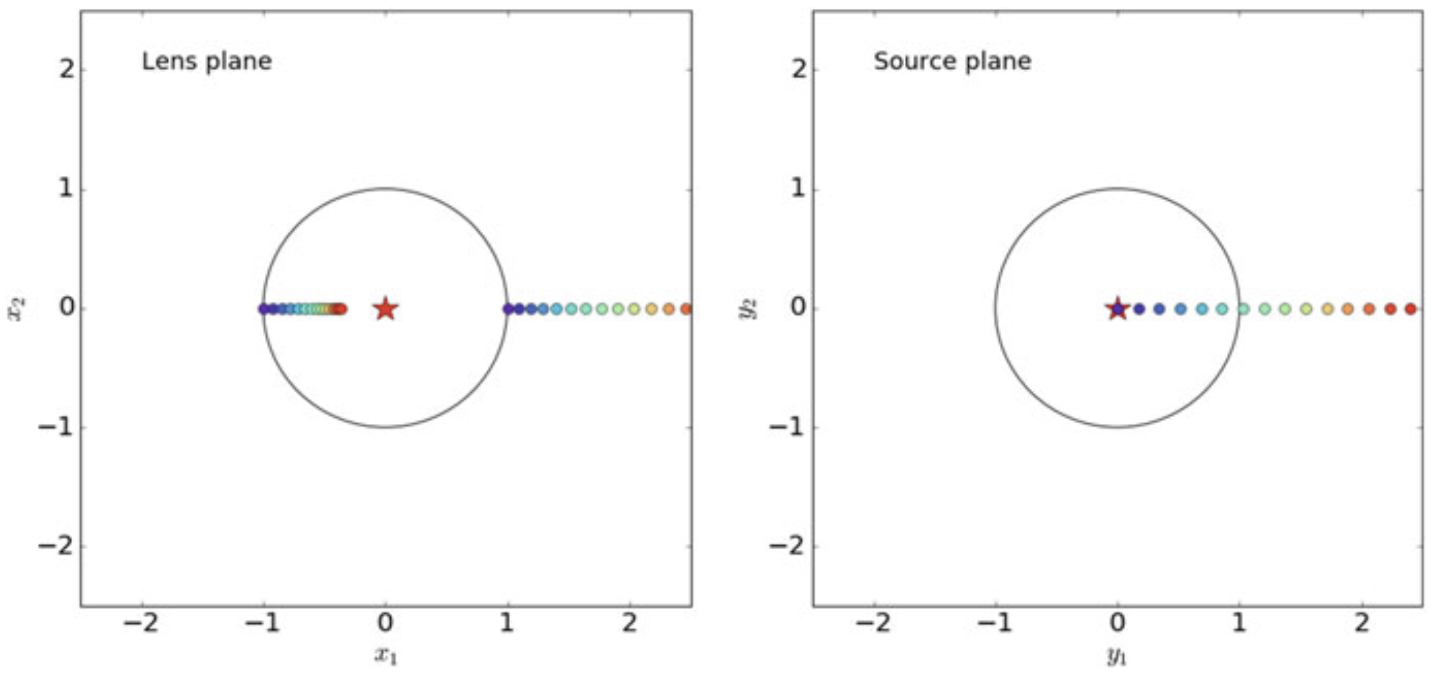
\includegraphics[width=\linewidth, keepaspectratio]{img//chapter3/pointmass_solutions.png}
    \caption[Lens equation solutions for point-mass lens]{Solutions of the lens equation for a point-mass, with the lens represented by the star at the center. The Einstein ring is highlighted in black. In the right diagram, the locations of various sources are marked with colored circles. The images produced, as calculated using \cref{eq:3.5}, are displayed in the left diagram.\\\small{Credits: \cite{meneghetti_introduction_2021}.}}
    \label{fig:pointmass_solutions}
\end{figure}

In the right section of \cref{fig:pointmass_solutions}, some sources are arranged at varying angular distances from the lens, which is marked by a red star. Each source is represented by a unique color to facilitate the identification of its corresponding images in the left section. Each source generates two images: one positioned at $x_+ > 0$ and the other in the range of $-1 < x_- < 0$. These images appear on either side of the lens, with the $x_-$ image always lying within a circle of radius $x = 1$. This circle is equivalent to the image produced by a source directly behind the point lens at $y = 0$, resulting in a ring-shaped image with radius $\t_E$, the Einstein ring.
The size of the Einstein radius is typically
\be
\label{eq:3.6}
\t_E \approx \SI{1}{\arcsecond} \bp{\frac{M}{10^{12} M_\odot}}^{1/2} \bp{\frac{D}{\si{\giga\parsec}}}^{-1/2} \,,
\ee
where
\be
\label{eq:3.7}
D \equiv \dfrac{D_L D_S}{D_{LS}}
\ee
is the \emph{effective lensing distance}.

As the angular separation $y \rightarrow 0$, it is observed that $x_- \rightarrow 0$, whereas $x_+ \rightarrow y$. This indicates that when the angular distance between the lens and the source increases significantly, the source is unlensed. In theory, an image still exists at $x_- = 0$, but this central image has zero magnification.


%%%%%%%%%%%%%%%%%%%%%%%%%%%%%%%%%%%%%%%%%%%%%%%%%%%%%%%
%%%%% Critical lines, caustics and magnification %%%%%
%%%%%%%%%%%%%%%%%%%%%%%%%%%%%%%%%%%%%%%%%%%%%%%%%%%%%%%
\subsection{Critical lines, caustics and magnification}
\label{subsec:critlines_caustics}
The Jacobian determinant for a point-mass lens can be written as
\be
\label{eq:3.8}
\det A (x) = \frac{y}{x} \frac{\dd{y}}{\dd{x}} \,,
\ee
which means that the eigenvalues of the Jacobian matrix are
\begin{subequations}
\begin{align}
    \label{eq:3.9a}
    \l_t (x) & = \frac{y}{x} = \bp{1 - \frac{1}{x^2}} \,,
    \\
    \label{eq:3.9b}
    \l_r (x) & = \frac{\dd{y}}{\dd{x}} = \bp{1 + \frac{1}{x^2}} \,.
\end{align}
\end{subequations}

The second eigenvalue is never zero, and therefore the point-mass lens only has a tangential critical line, a circle with equation $x^2 = 1$, which represents the Einstein ring.
This line can be mapped onto the source plane to find the relative tangential caustic, resulting in a single point at $y = 0$.

Given that the magnification is the inverse of the Jacobian determinant
\be
\label{eq:3.10}
\m (x) = \bp{1 - \frac{1}{x^4}}^{-1} \,,
\ee
which can also be written as a function of the source position
\be
\label{eq:3.11}
\m_\pm (y) = \frac{x}{y} \frac{\dd{x}}{\dd{y}} = \frac{1}{2} \bp{1 \pm \frac{y^2 + 2}{y \sqrt{y^2 + 4}}} \,,
\ee
the magnifications of the two images always have the same signs of $x_\pm$ and therefore different parity.

The total source magnification will then be:
\be
\label{eq:3.12}
\m (y) = \m_+ (y)  + |\m_- (y)| = \frac{y^2 + 2}{y \sqrt{y^2 + 4}} \,,
\ee
while the sum of the signed magnifications is always $\m = 1$.

Furthermore, it can be shown through series expansion that, for large $y$,
\be
\label{eq:3.13}
\lim_{y\to\infty} \left| \frac{\m_+}{\m_-} \right| \propto y^4 \,.
\ee
This means that the magnification rapidly becomes negligible outside the Einstein ring and has a very simple form well inside it. Hence, deviations from simple point-lens microlensing can usually be easily spotted.


%%%%%%%%%%%%%%%%%%%%%%%%%%%%%%%%%%%%%%%%%%%%%%%%%%%%%%%
%%%%% Microlensing light-curve %%%%%
%%%%%%%%%%%%%%%%%%%%%%%%%%%%%%%%%%%%%%%%%%%%%%%%%%%%%%%
\subsection{Microlensing light-curve}
\label{subsec:micro_lc}
The Einstein radius of a typical lens indicates the scale of image separation observed in microlensing events. For a star with the mass of the Sun located within the Milky Way, the separation is approximately of the order of milliarcseconds, a measurement that is beyond the detection capabilities of current instruments. However, stars move around the Galactic center (and have an additional random velocity component with respect to one another). The relative velocities are such that the time scale of the relative change of lens and source positions is of order of weeks or shorter. Therefore, this motion introduces a temporal component in the lensing geometry, causing the distance between the lens and the source, and thus the magnification, to vary measurably as a function of time, accordingly to \cref{eq:3.12}. In general, a source with intrinsic flux $F_s$ will appear to have flux $F (t) = \m (t) F_s$. 
\newpage
The \emph{microlensing light-curve} describes the temporal behavior of the magnification, dictated by the relative motion of the lens across the observer-source line of sight.

\begin{figure}
    \centering
    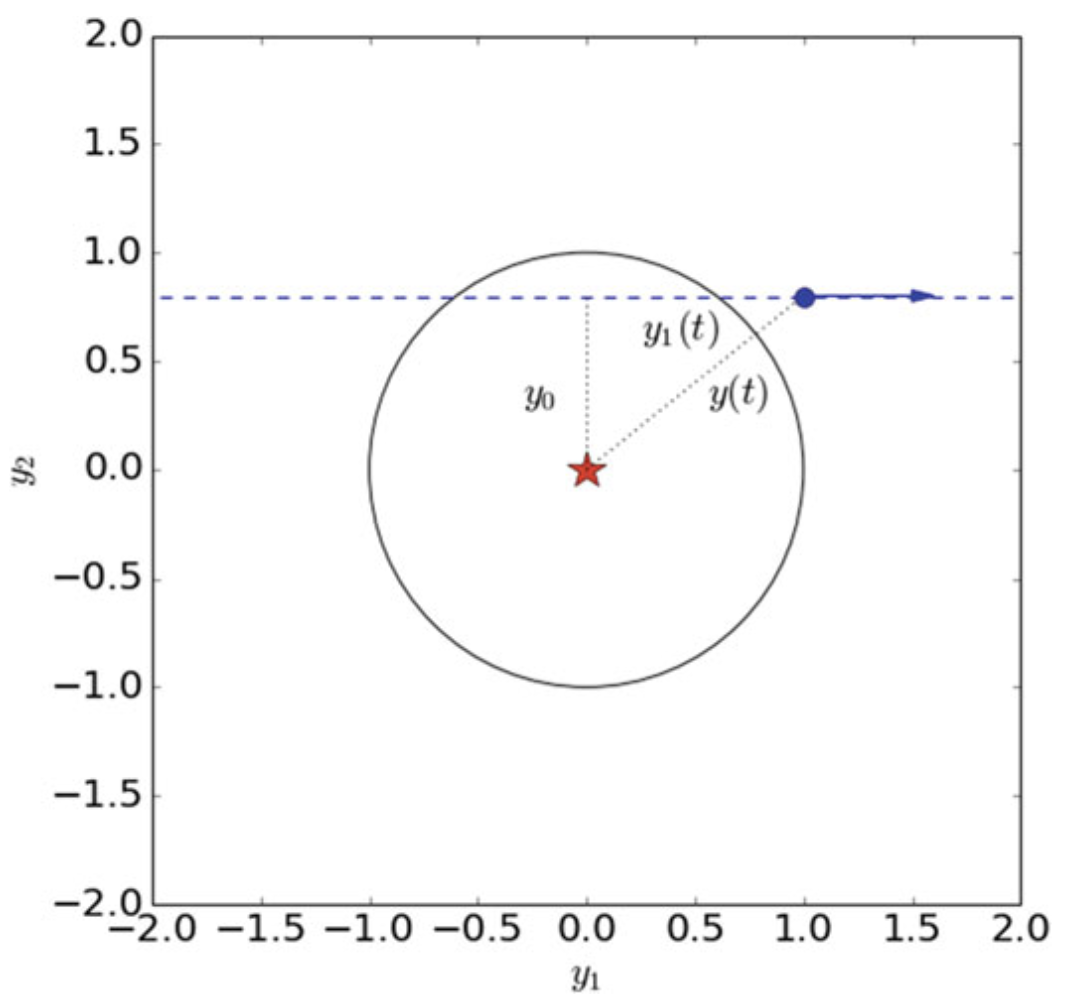
\includegraphics[width=0.61\linewidth, keepaspectratio]{img//chapter3/lens_source_trajectory.png}
    \caption[Lens position and source trajectory in a microlensing event]{Illustration of the lens position and source trajectory. The dimensionless impact parameter is $y_0$, $y_1 (t)$ indicates the dimensionless distance of the source from its closest point to the lens, and $y (t)$ is the dimensionless distance between the lens and source.\\\small{Credits: \cite{meneghetti_introduction_2021}.}}
    \label{fig:lens_source_trajectory}
\end{figure}

As shown in \cref{fig:lens_source_trajectory}, assuming a straight line can approximate the path of the source relative to the lens, the former moving with transverse velocity $v$ and reaching the minimum dimensionless distance $y_0$ (\ie the \emph{impact parameter} of the source), from the lens at time $t_0$, the dimensionless distance of the source from $y_0$ can be written
\be
\label{eq:3.14}
y_1 (t) = \frac{v (t - t_0)}{D_L \t_E} \,.
\ee

Since magnification significantly deviates from unity only for sources with $|y| \lesssim 1$, the characteristic timescale of the microlensing event is given by
\be
\label{eq:3.15}
t_E = \frac{D_L \t_E}{v} \,,
\ee
which is known as the \emph{Einstein crossing time}. Stellar lenses in the Milky Way are associated with typical $t_E$ on the order of a month, and thus the changes in the observed brightness of the source they induce are referred to as microlensing ``events''.

Inserting \cref{eq:3.15} into \cref{eq:3.14}, the trajectory of the source can be represented by
\be
\label{eq:3.16}
y (t) = \sqrt{y_0^2 + y_1^2 (t)} = \sqrt{y_0^2 + \frac{(t - t_0)^2}{t_E^2}}  \,.
\ee

The corresponding light-curve of the source, examples of which are shown in \cref{fig:light_curves}, is then obtained by combining \cref{eq:3.16,eq:3.12} and multiplying by the unlensed source flux
\be
\label{eq:3.17}
F (t) = \m (t) F_s = \frac{y (t)^2 + 2}{y (t) \sqrt{y (t)^2 + 4}} F_s  \,.
\ee

\begin{figure}
    \centering
    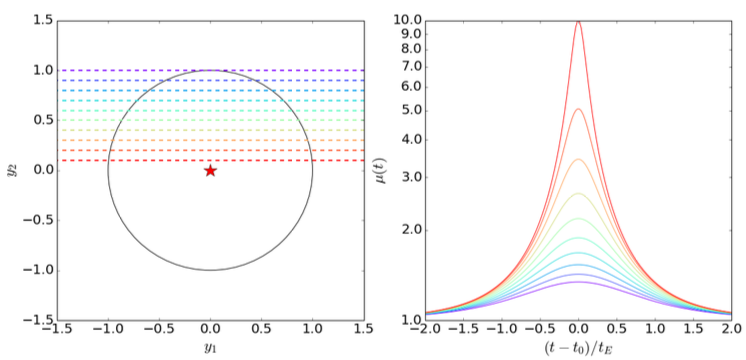
\includegraphics[width=\linewidth, keepaspectratio]{img//chapter3/light_curves.png}
    \caption[Microlensing light-curves for different impact parameters]{Left panel: some examples of source trajectory across the Einstein ring with different impact parameters $y_0$. Right panel: corresponding light-curves.\\\small{Credits: \cite{meneghetti_introduction_2021}.}}
    \label{fig:light_curves}
\end{figure}

The \emph{standard} microlensing light-curve of a simple point-source, point-lens system is thus described by four parameters: unlensed flux $F_s$, $t_0$, $y_0$ and $t_E$. Of these, $F_s$ can be measured in the absence of microlensing, $t_0$ and $y_0$ from the position and height of the light-curve peak, respectively. Only $t_E= D_L \t_E / v$ contains physical information about the lens system and determines the peak width, \ie the duration of the event. Assuming that the source distance can be determined from its properties (membership in a stellar system, spectral type and apparent magnitude), there are three physical parameters, lens mass $M$, lens distance $D_L$, and lens relative transverse velocity $v$, to determine from one observable: this is the so-called \emph{microlensing degeneracy}. 
Although the standard light-curve model is successful in numerous instances, there exist circumstances where some foundational assumptions of this model no longer hold. In such situations, it might be feasible to derive additional constraints that can partially lift the degeneracy. Non-standard light-curves, for instance, may occur when either the source or the lens are not point-like, or when the path of the source moving relative to the lens is not linear. Such instances often occur when either the lens or the source, or both, are part of binary systems.

% *************************************************************
%%%%% SECTION 3.2: EXTENDED LENSES %%%%%
\section{Extended lenses}
\label{sec:ext_lenses}
This section aims to introduce the main models used to represent extended gravitational lenses, such as massive galaxies and galaxy clusters. These cosmic structures, characterized by their complex, gravitationally bound mass distributions, are formidable gravitational lenses capable of producing striking lensing phenomena, including multiple images and gravitational arcs.

The analysis starts with circular, axially symmetric models and describes how different mass profiles affect lensing properties. Subsequently, deviations from circular symmetry are introduced through properties such as ellipticity and substructures. Finally, the impact of the environment surrounding the lenses is taken into account. The thin screen approximation is used throughout this description of analytical lens models.


%%%%%%%%%%%%%%%%%%%%%%%%%%%%%%%%%%%%%%%%%%%%%%%%%%%%%%%
%%%%% Axially symmetric profiles %%%%%
%%%%%%%%%%%%%%%%%%%%%%%%%%%%%%%%%%%%%%%%%%%%%%%%%%%%%%%
\subsection{Axially symmetric profiles}
\label{subsec:axially_profiles}
The most simple description of an extended lens is an axially symmetric profile. For such lenses, the potential is constant on circles centered on the lens center. This symmetry allows most equations to be simplified to a one-dimensional form.

The deflection angle is radially directed and its amplitude depends only on the distance from the lens center. Its expression is the same as that of the point-mass lens, with the only difference that now $M = M(\t)$ is the mass enclosed in a circle of radius $\t$. For this reason, introducing an arbitrary reference scale $\x_0$, the \emph{dimensionless mass} profile can be written as
\be
\label{eq:3.18}
m (x) = 2 \int_0^x x^\prime \k (x^\prime) \dd{x^\prime} = \frac{M (\x_0 x)}{\pi \x_0^2 \S_{cr}} \,, 
\ee
which leads to a deflection angle
\be
\label{eq:3.19}
\a (x) = \frac{2}{x} \int_0^x x^\prime \k (x^\prime) \dd{x^\prime} = \frac{m (x)}{x} \,.
\ee

Therefore, the lens equation is
\be
\label{eq:3.20}
y = x - \frac{m (x)}{x} \,.
\ee

Given that $\P^\prime (x) = \a (x)$, from \cref{eq:2.17} the convergence profile can be obtained:
\be
\label{eq:3.21}
\k (x) = \frac{1}{2} \bs{\a^\prime (x) + \frac{\a (x)}{x}} = \frac{m^\prime (x)}{2 x} \,.
\ee

Finally, introducing $\overline{\k} (x) = m (x) / x^2$ as the mean convergence within a circle of radius $x$, the shear vector results
\be
\label{eq:3.22}
\g (x) = \frac{1}{2} \left| \a^\prime (x) - \frac{\a (x)}{x} \right| = |\k (x) - \overline{\k} (x)| \,.
\ee

Using the precedent results and \cref{eq:2.24}, it is possible to compute the determinant of the lensing Jacobian
\be
\label{eq:3.23}
\det A (x) = \frac{y}{x} \frac{\dd{y}}{\dd{x}} = [1 - \k (x) - \g (x)] [1 - \k (x) + \g (x)] \,,
\ee
and the correspondent magnification profile $\m (x) = [\det A (x)]^{-1}$.

As described in \cref{sec:lens_equation}, the set of points that satisfies $\det A (x) = 0$ represents the critical lines of the lens. For an axially symmetric lens these are circles, whose radii can be found by solving the equations
\begin{subequations}
\begin{align}
    \label{eq:3.24a}
    \l_t (x) & = 0 \quad \Rightarrow \quad \k (x) + \g (x) = 1 \,,
    \\
    \label{eq:3.24b}
    \l_r (x) & = 0 \quad \Rightarrow \quad \k (x) - \g (x) = 1 \,,
\end{align}
\end{subequations}
which define the \emph{tangential critical line} and the \emph{radial critical line}, respectively.

Through the lens equation, it can be seen that all the points along the tangential critical line are mapped to the point $y = 0$ on the source plane: this type of lenses have point-like tangential caustics. Instead, the radial critical points are mapped onto a circular radial caustic on the source plane.


%%%%%%%%%%%%%%%%%%%%%%%%%%%%%%%%%%%%%%%%%%%%%%%%%%%%%%%
%%%%% Power-law profiles %%%%%
%%%%%%%%%%%%%%%%%%%%%%%%%%%%%%%%%%%%%%%%%%%%%%%%%%%%%%%
\subsection{Power-law profiles}
\label{subsec:power_law_profiles}
This class of lenses is characterized by a mass profile with a power-law form of the kind
\be
\label{eq:3.25}
m (x) = x^{3-n} \,,
\ee
where $n$ is a parameter that can assume any real value $>1$.

From the previous mass profile definition, all the other lensing properties can be derived:
\begin{equation}
\label{eq:3.26}
\begin{aligned}
    \k (x) & = \frac{m^\prime (x)}{2 x} = \frac{3 - n}{2} x^{1 - n} \,, \\[5pt]
    \a (x) & = \frac{m (x)}{x} = x^{2 - n} \,, \\[5pt]
    \g (x) & = \left| \frac{m^\prime}{2 x} - \frac{m (x)}{x^2} \right| = \frac{n - 1}{2} x^{1 - n} \,, \\[5pt]
    y & = x - x^{2-n} \,.
\end{aligned}
\end{equation}

In particular, given the value of the parameter $n$, it is possible to distinguish different scenarios.
\begin{itemize}
    \item \textbf{n = 1}: perfectly convergent lens with constant convergence and $y (x) = 0$, $\forall x$;
    
    \item \textbf{1 < n < 2}: mass and deflection angle profiles increase with $x$, while the convergence and shear profiles show a decrease. The tangential critical line forms a circle of radius $x_t = 1$, $\forall n$, and its corresponding caustic line is a single point at $y_t = 0$. On the other hand, the size of the radial critical line varies according to the value of $n$. As it increases, the radial critical line becomes smaller, whereas the size of the caustic line follows an increasing trend. In particular, for $n = 2$, the radial critical line is absent. For lenses that are axially symmetric, there are multiple methods to solve the lens equation, but the most effective approach is often referred to as the \emph{image diagram}, by which multiple image positions can be identified where the profile of the deflection angle intersects the lines $f(x) = x - y$.
    
    \Cref{fig:image_diagrams_1_2} demonstrates that the separation between images is influenced by the value of $n$: a higher value results in a more curved profile of the deflection angle, leading to a greater number of images that are closer together, and conversely, a lower $n$ leads to fewer images with larger separations. More precisely, these lenses produce three images if the source is inside the radial critical line (\ie $\,y < y_r$), otherwise they form a single image.
    
    \item \textbf{n = 2}: flat deflection angle profile, Singular Isothermal Sphere model (see \cref{subsec:sis});
    
    \item \textbf{n > 2}: deflection angle profile decreases with $x$ and has a singularity in $x = 0$. These lenses produce two images, one inside and one outside the Einstein radius (see \cref{fig:image_diagrams_2}). The radial eigenvalue is always non-zero, causing the absence of a radial critical line and ensuring that the radial magnification factor, $\m_r < 1$, always. This means that the images are consistently demagnified in the radial direction.
    
    It should be noted that for $n = 3$ the scenario corresponds to that of a point-mass lens.
\end{itemize}

\begin{figure}[h!]
    \centering
    \includegraphics[width=\linewidth, keepaspectratio]{img//chapter3/image_diagrams_1_2.png}
    \caption[Image diagrams for power-law lenses with $1<n<2$]{Image diagrams for different values of $1<n<2$. The solid curves show the function $\a (x)$, while the dashed lines represent the function $f (x) = x - y$, with varying $y$ value.}
    \label{fig:image_diagrams_1_2}
\end{figure}

\begin{figure}[h!]
    \centering
    \includegraphics[width=\linewidth, keepaspectratio]{img//chapter3/image_diagrams_2.png}
    \caption[Image diagrams for power-law lenses with $n>2$]{Image diagrams for different values of $n>2$. The solid curves show the function $\a (x)$, while the dashed lines represent the function $f (x) = x - y$, with varying $y$ value.}
    \label{fig:image_diagrams_2}
\end{figure}


%%%%%%%%%%%%%%%%%%%%%%%%%%%%%%%%%%%%%%%%%%%%%%%%%%%%%%%
%%%%% Singular Isothermal Sphere %%%%%
%%%%%%%%%%%%%%%%%%%%%%%%%%%%%%%%%%%%%%%%%%%%%%%%%%%%%%%
\subsection{Singular Isothermal Sphere}
\label{subsec:sis}
One of the simplest and most widely used models for axially symmetric lenses is the Singular Isothermal Sphere (SIS). The density profile is obtained by assuming that the matter constituting the lens acts like an ideal gas, contained within a spherically symmetric gravitational potential. This gas is presumed to be in states of thermal and hydrostatic equilibrium.

By projecting the three-dimensional density onto the lens plane, the surface mass density can be calculated
\be
\label{eq:3.27}
\S (\x) = \int_0^\infty \r (\x, z) \dd{z} = \frac{\s_v^2}{2 G \x} \,,
\ee
where $\x$ is the distance from the center of the lens and $\s_v$ represents the gas particle velocity dispersion (\ie the stars in a galaxy or the galaxies in a cluster).
Although this profile is not physical, having a singularity for $\x = 0$ and an infinite total mass, it reproduces very well the observed flat rotation curves of spiral galaxies for $0 \ll \x < \infty$.

Setting the length scale at $\x_0 = 4 \pi \bp{\frac{\s_v}{c}}^2 \frac{D_L D_{LS}}{D_S}$, it is possible to rewrite \cref{eq:3.27} in a dimensionless form and derive the convergence profile
\be
\label{eq:3.28}
\S (x) = \frac{\S_{cr}}{2 x} \quad \Rightarrow \quad \k (x) = \g (x) = \frac{1}{2 x} \,,
\ee
which shows that the SIS lens corresponds to a power-law lens with $n=2$.

From the convergence definition, the deflection angle and the lens equation can be obtained:
\begin{subequations}
\begin{align}
    \label{eq:3.29a}
    &\a (x) = \frac{x}{|x|} \,,
    \\
    \label{eq:3.29b}
    &y = x - \frac{x}{|x|} \,.
\end{align}
\end{subequations}

The solutions of the lens equation are dependent on the source position $y$, as it can be seen in the left panel of \cref{fig:image_diagrams_2}:
\begin{itemize}
    \item when $0 < y < 1$ there exist two solutions on opposite sides of the lens center; one is at $x_- = y - 1$ and one at $x_+ = y + 1$. Their angular separation is always $\D (\t_E) = 2 \t_E$;

    \item when $y > 1$ there is only one solution at $x_+ = y + 1$.
\end{itemize}

Therefore, the circle of radius $y = 1$ serves a similar function to that of the radial caustic for power-law lenses with $1 < n < 2$, delineating areas on the source plane that are associated with different image multiplicities. However, this circle does not qualify as caustic because $\a^\prime (x) = 0$, $\forall x$, indicating that $\l_r = 1$. Instead, the circle of radius $y_{cut} = 1$ is referred to as pseudo-caustic, known as the \emph{cut}. In addition, unlike ''normal" caustics, the number of images changes only by one when crossing the cut, instead of changing by two.

Given that $\l_r = 1$, the images are only magnified in the tangential direction, while the radial size of all the images remains unchanged. In particular, when the source is placed inside the cut, the magnifications can be expressed as:
\begin{subequations}
\begin{align}
    \label{eq:3.30a}
    \m_- (y) & = 1 - \frac{1}{y} \,,
    \\
    \label{eq:3.30b}
    \m_+ (y) & = 1 + \frac{1}{y} \,,
\end{align}
\end{subequations}
for the image inside and outside the Einstein ring respectively.

From \cref{eq:3.30a,eq:3.30b} can be seen that for $y \rightarrow 1$ the image $x_-$ becomes weaker and weaker until it disappears for $y = 1$. On the other hand, when $y \rightarrow \infty$ the source magnification tends to unity: sources at a large distance from the lens experience little to no magnification.

\Cref{fig:sis_extended} shows some examples of images produced by a SIS lens of an extended circular source, placed at different distances from the lens.

\begin{figure}
    \centering
    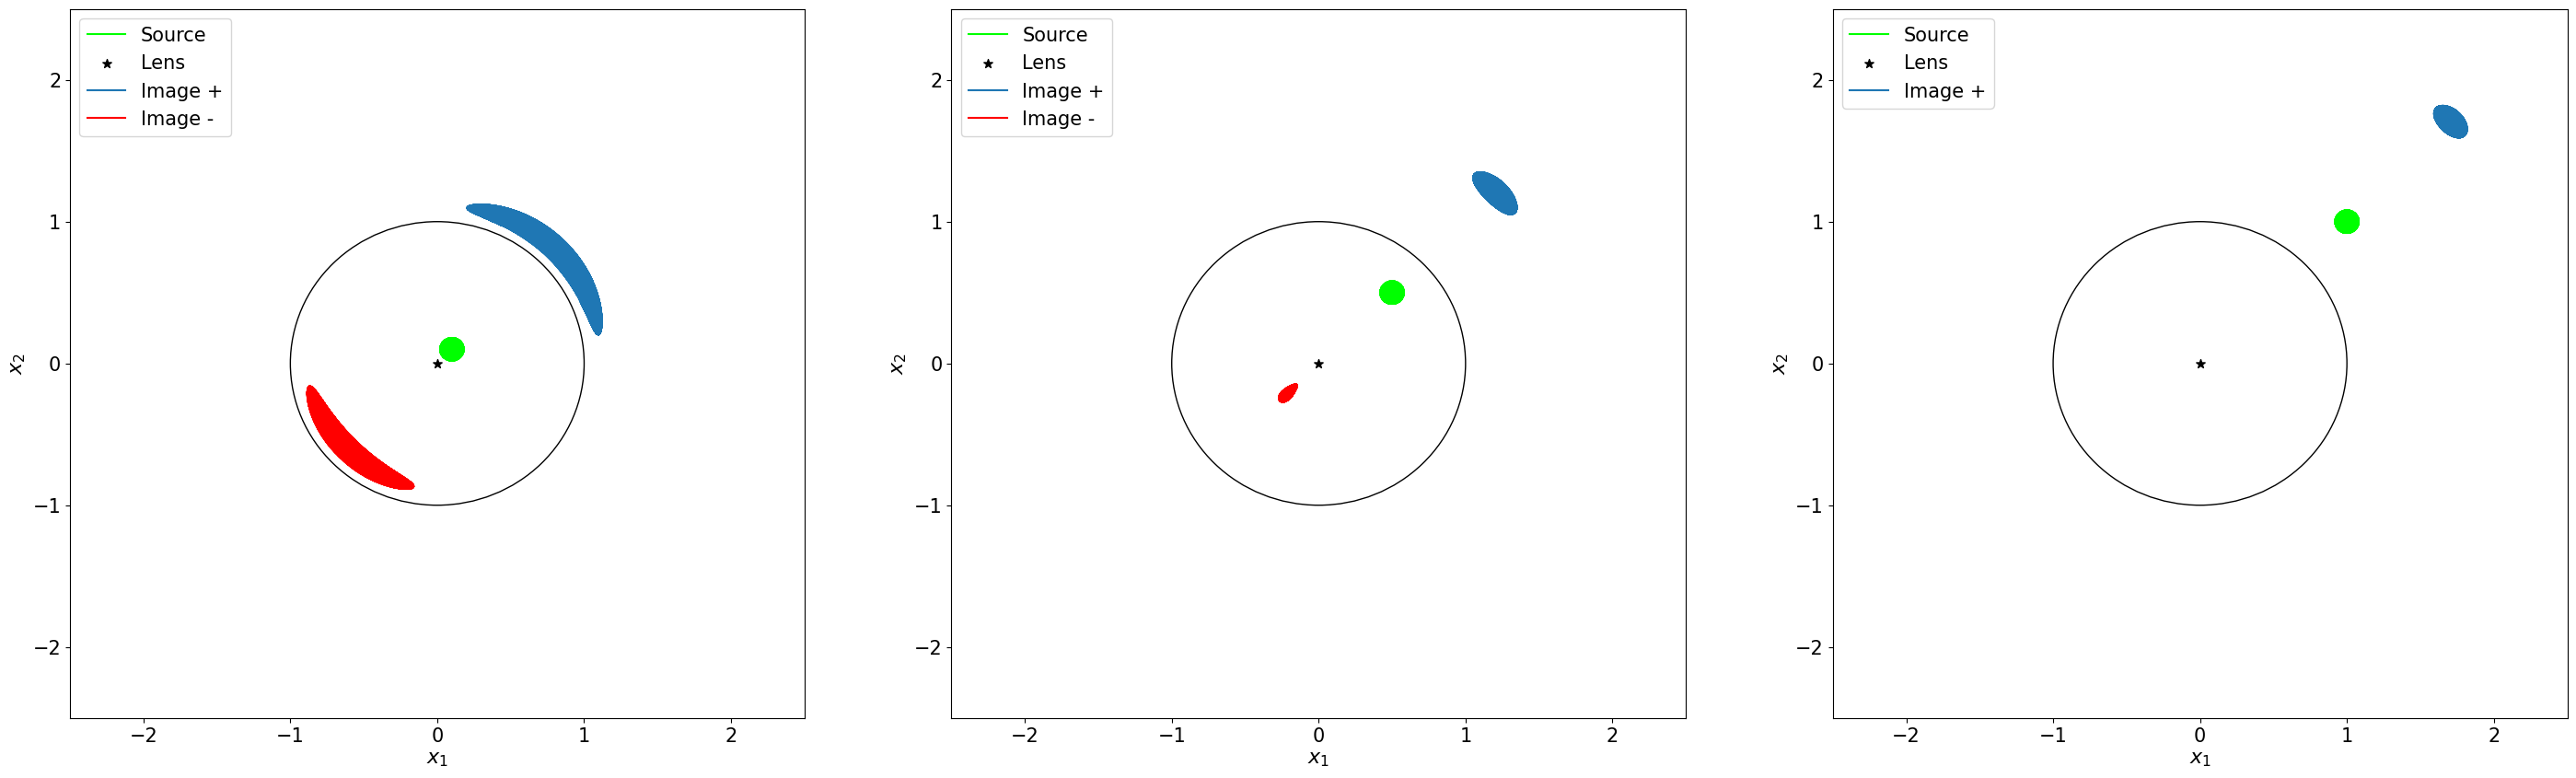
\includegraphics[width=\linewidth, keepaspectratio]{img//chapter3/sis_extended.png}
    \caption[Imaging of an extended source by a SIS lens]{Imaging of an extended source by a SIS lens. Each panel shows the images produced for different values of $y$. The black circle represents the tangential critical line of the lens, the Einstein ring.}
    \label{fig:sis_extended}
\end{figure}


%%%%%%%%%%%%%%%%%%%%%%%%%%%%%%%%%%%%%%%%%%%%%%%%%%%%%%%
%%%%% Non-singular Isothermal Sphere %%%%%
%%%%%%%%%%%%%%%%%%%%%%%%%%%%%%%%%%%%%%%%%%%%%%%%%%%%%%%
\subsection{Non-singular Isothermal Sphere}
\label{subsec:nis}
One way to solve the central singularity issue of the SIS lens is to introduce an additional parameter $\x_c$, describing a flat central core of the surface density profile \citep{kormann_isothermal_1994}:
\be
\label{3.31}
\S (\x) = \frac{\S_0}{\sqrt{1 + (\x / \x_c)^2}} \quad \mathrm{with} \quad \S_0 = \frac{\s_v^2}{2 G \x_c} \,,
\ee
where $\S_0$ represents the constant surface density for $\x \ll \x_c$.

By introducing the same scale length $\x_0$ defined in \cref{subsec:sis} and re-scaling both $\x$ and $\x_c$, the dimensionless relevant quantities for the Non-singular Isothermal Sphere (NIS) can be derived:
\begin{equation}
\label{eq:3.32}
\begin{aligned}
    &\k (x) = \frac{1}{2 \sqrt{x^2 + x_c^2}} \,, \\[5pt]
    &\m (x) = \sqrt{x^2 + x_c^2} - x_c \,, \\[5pt]
    &\a (x) = \sqrt{1 + \bp{\frac{x_c}{x}}^2} - \frac{x_c}{x} \,, \\[5pt]
    &y = x - \sqrt{1 + \bp{\frac{x_c}{x}}^2} - \frac{x_c}{x} \,.
\end{aligned}
\end{equation}

The lens equation above can be reduced to a third-order polynomial: the NIS lens can produce up to three images of a given source, with multiplicity depending on the value of $x_c$. It can be shown \citep{meneghetti_introduction_2021} that tangential and critical lines exist only for values of $x_c < 1/2$, \ie for $x_c > 1/2$ the lens is ``weak'' and cannot produce multiple images.
In particular, the tangential caustic is a point at $y_t = 0$, while the radii of the tangential critical line, the radial caustic and the radial critical line vary with $x_c$ as shown in \cref{fig:nis_radii}. 

\begin{figure}[b!]
    \centering
    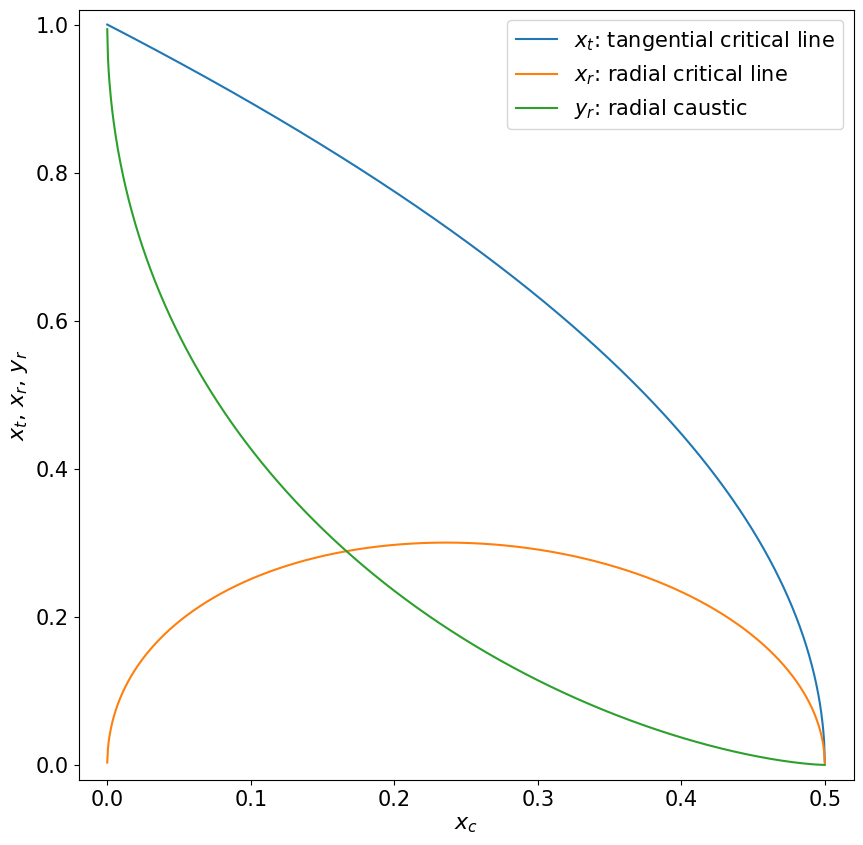
\includegraphics[width=0.65\linewidth]{img//chapter3/nis_radii.png}
    \caption[NIS caustic critical lines radii as a function of $x_c$]{NIS caustic critical lines radii as a function of $x_c$. For $x_c = 0$, $y_r = 1$, \ie the SIS cut.}
    \label{fig:nis_radii}
\end{figure}


%%%%%%%%%%%%%%%%%%%%%%%%%%%%%%%%%%%%%%%%%%%%%%%%%%%%%%%
%%%%% Singular Isothermal Ellipsoid %%%%%
%%%%%%%%%%%%%%%%%%%%%%%%%%%%%%%%%%%%%%%%%%%%%%%%%%%%%%%
\subsection{Singular Isothermal Ellipsoid}
\label{subsec:sie}
After investigating the impact of altering the slope of the density profile and the incorporation of a central core, it is possible to assess the influence of ellipticity on lens characteristics. Introducing ellipticity surely improves the representation of galaxies and their mass distributions. \cite{kormann_isothermal_1994} developed the Singular Isothermal Ellipsoid (SIE) model, which can be derived from the SIS model by substituting
\be
\label{eq:3.33}
\x \quad \Rightarrow \quad \sqrt{\x_1^2 + f^2 \x_2^2} \,,
\ee
where $0 < f \leq 1$ is the axis ratio of the ellipses that, in this scenario, define the iso-density contours of the mass profile.

Through this substitution, the surface density profile becomes
\be
\label{eq:3.34}
\S (\va{\x}) = \frac{\s_v^2}{2 G} \frac{\sqrt{f}}{\sqrt{\x_1^2 + f^2 \x_2^2}}  \,,
\ee
which, as already said, is constant on ellipses with minor axis $\x$ and major axis $\x / f$.

By choosing, once again, the same scale length $\x_0$ as for the SIS model, the convergence can be written as
\be
\label{eq:3.35}
\k (\vec{x}) = \frac{\sqrt{f}}{2 \sqrt{x_1^2 + f^2 x_2^2}}  \,,
\ee
or, using polar coordinates,
\be
\label{eq:3.36}
\k (x, \varphi) = \frac{\sqrt{f}}{2 x \D (\varphi)}  \,,
\ee
where
\be
\label{eq:3.37}
\D (\varphi) = \sqrt{\cos{(\varphi)}^2 + f^2 \sin{(\varphi)}^2}  \,.
\ee

By solving the Poisson equation, the lensing potential in polar coordinates can be obtained, and then, taking its gradient, it is possible to derive the deflection angle, which has two components, none of which depends on $x$:
\begin{equation}
\begin{aligned}
    \label{eq:3.38}
    \a_1 (\vec{x}) & = \sqrt{\frac{f}{1 - f^2}} \arcsinh \bp{\frac{\sqrt{1 - f^2}}{f} \cos{(\varphi)}} \,,
    \\
    \a_2 (\vec{x}) & = \sqrt{\frac{f}{1 - f^2}} \arcsin \bp{\sqrt{1 - f^2} \sin{(\varphi)}} \,.
\end{aligned}
\end{equation}

The shear components can be obtained from the derivatives of the deflection angle
\begin{equation}
\begin{aligned}
    \label{eq:3.39}
    \g_1 (\vec{x}) & = - \k (\vec{x}) \cos{(2 \varphi)} \,,
    \\
    \g_2 (\vec{x}) & = - \k (\vec{x}) \sin{(2 \varphi)} \,,
\end{aligned}
\end{equation}
and, as for the SIS model, $\g = \sqrt{\g_1^2 + \g_2^2} = \k$.

Finally, from the lensing Jacobian determinant, the two eigenvalue are
\begin{subequations}
\begin{align}
    \label{eq:3.40a}
    \l_t (\vec{x}) & = 1 - 2 \k (\vec{x}) \,,
    \\
    \label{eq:3.40b}
    \l_r (\vec{x}) & = 1 \,.
\end{align}
\end{subequations}

Similarly to the SIS lens, the SIE does not have a radial critical line. Instead, the tangential critical line is the ellipse defined by
\be
\label{eq:3.41}
\k (\vec{x}) = \frac{1}{2} \quad \Rightarrow \quad \vec{x}_t (\varphi) = \frac{\sqrt{f}}{\D (\varphi)} [\cos{(\varphi)}, \sin{(\varphi)}] \,.
\ee

As always, the points on the critical line can be mapped onto the source plane using the lens equation: introducing ellipticity to the lens disrupts its axial symmetry, leading to the transformation of the tangential caustic from a central point into an astroid-shaped caustic, featuring four cusps and four folds. As for the SIS, due to the singularity at the center of the lens, also for the SIE profile does not exist a radial critical line and, as a result, the multiple images region is not enclosed by the radial caustic, but by the cut, which is an ellipse.

The number of multiple images formed by this lens is influenced by the positioning of the cut and caustic lines. In particular, for large ellipticities (small values of $f$, in particular $f < f_0 = 0.3942$), the tangential caustic extends outside the cut, as shown in \cref{fig:naked_cusps}. The cusps that are not contained within the cut are called \emph{naked}.

\begin{figure}
    \centering
    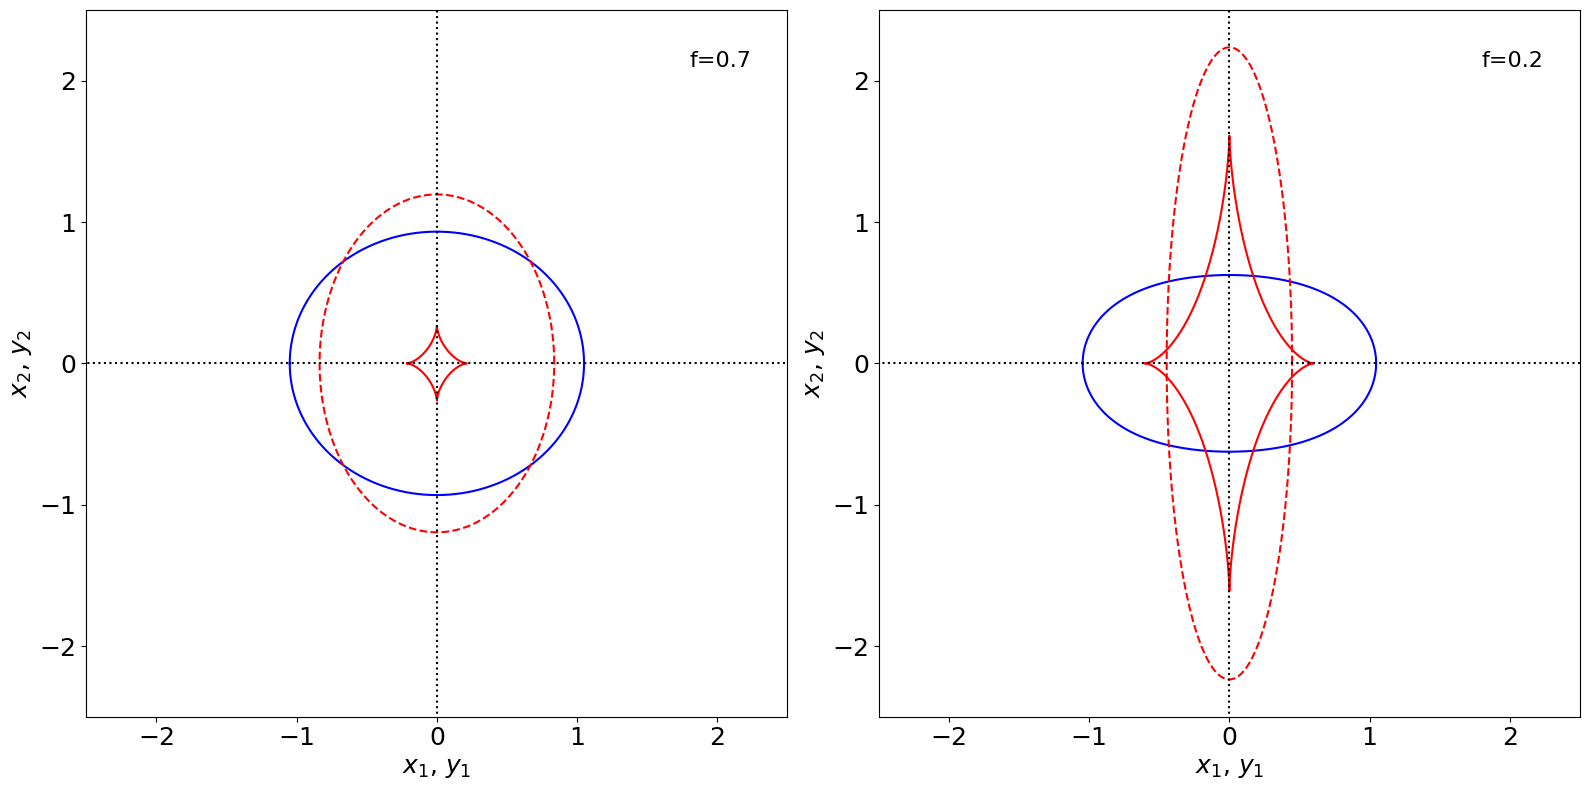
\includegraphics[width=\linewidth, keepaspectratio]{img//chapter3/naked_cusps.png}
    \caption[SIE caustics and critical lines]{Tangential critical line (dashed red), tangential caustic (solid red) and cut (solid blue) for two SIE lenses with $f = 0.7$ and $f = 0.2$.}
    \label{fig:naked_cusps}
\end{figure}

Given that crossing the cut alters the number of images by one and traversing the caustic alters it by two, the scenarios with $f > f_0$ are capable of generating one, two, or four images. In contrast, a smaller value of $f$ can lead to the existence of another possible scenario with the formation of three multiple images (see \cref{fig:sie}).

\begin{figure}
  \begin{minipage}{0.5\linewidth}
    \centering
    \subfloat[]{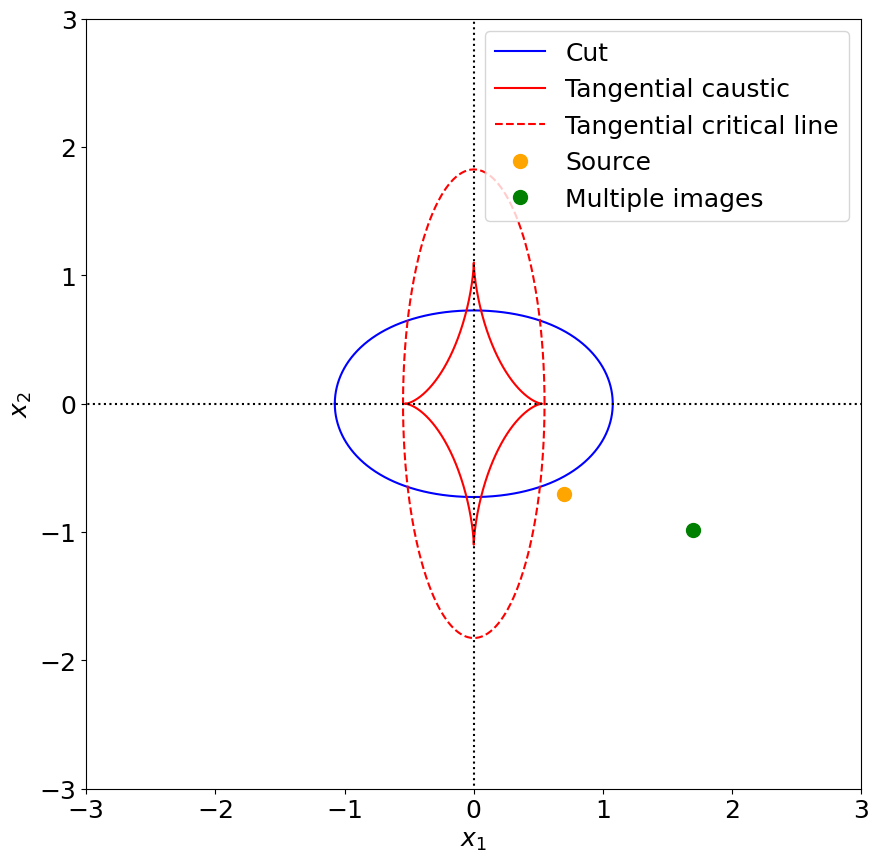
\includegraphics[width=\linewidth, keepaspectratio]{img/chapter3/sie1.png}\label{fig:sie1}}
  \end{minipage}%%
  \begin{minipage}{0.5\linewidth}
    \centering
    \subfloat[]{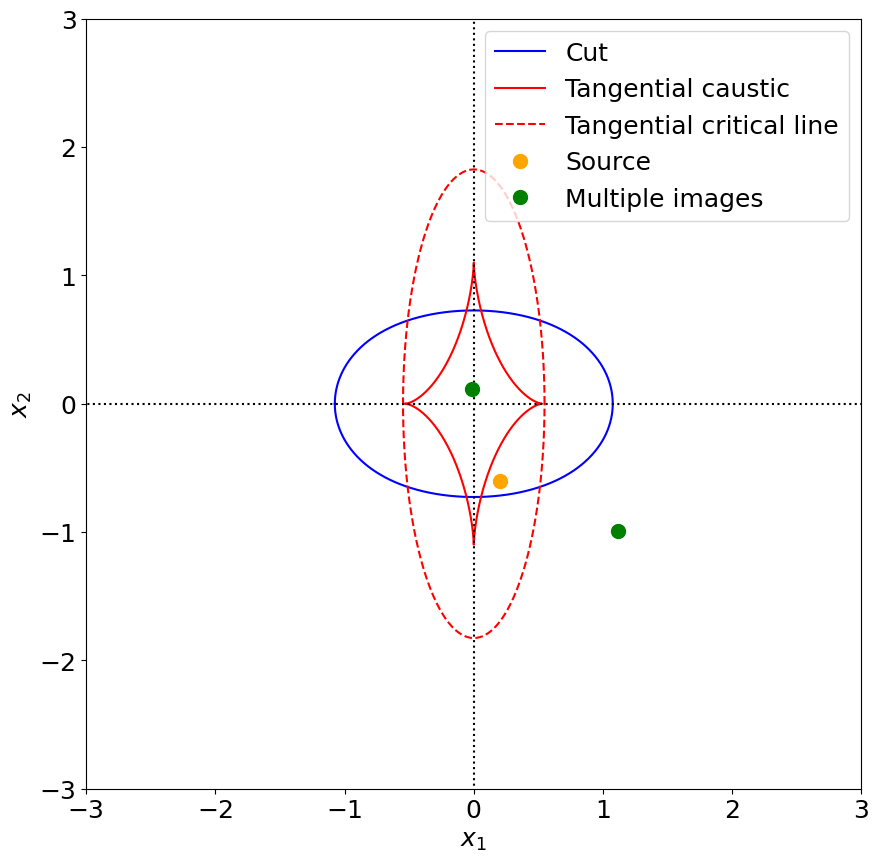
\includegraphics[width=\linewidth, keepaspectratio]{img/chapter3/sie2.png}\label{fig:sie2}}
  \end{minipage} 
  \begin{minipage}{0.5\linewidth}
    \centering
    \subfloat[]{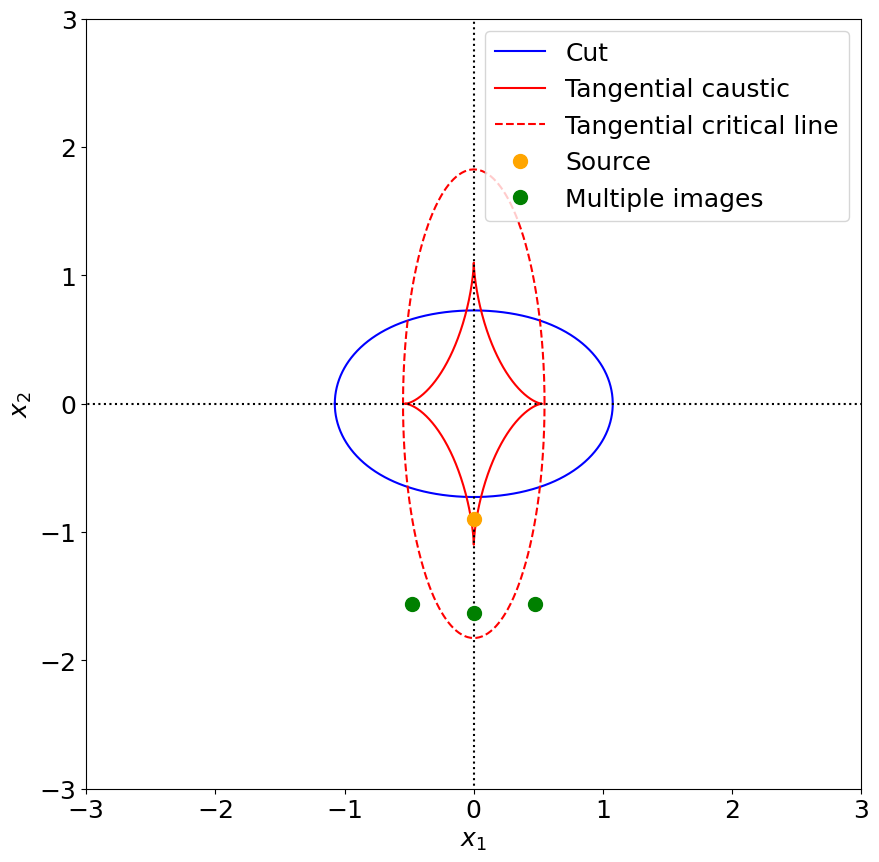
\includegraphics[width=\linewidth, keepaspectratio]{img/chapter3/sie3.png}\label{fig:sie3}}
  \end{minipage}%% 
  \begin{minipage}{0.5\linewidth}
    \centering
    \subfloat[]{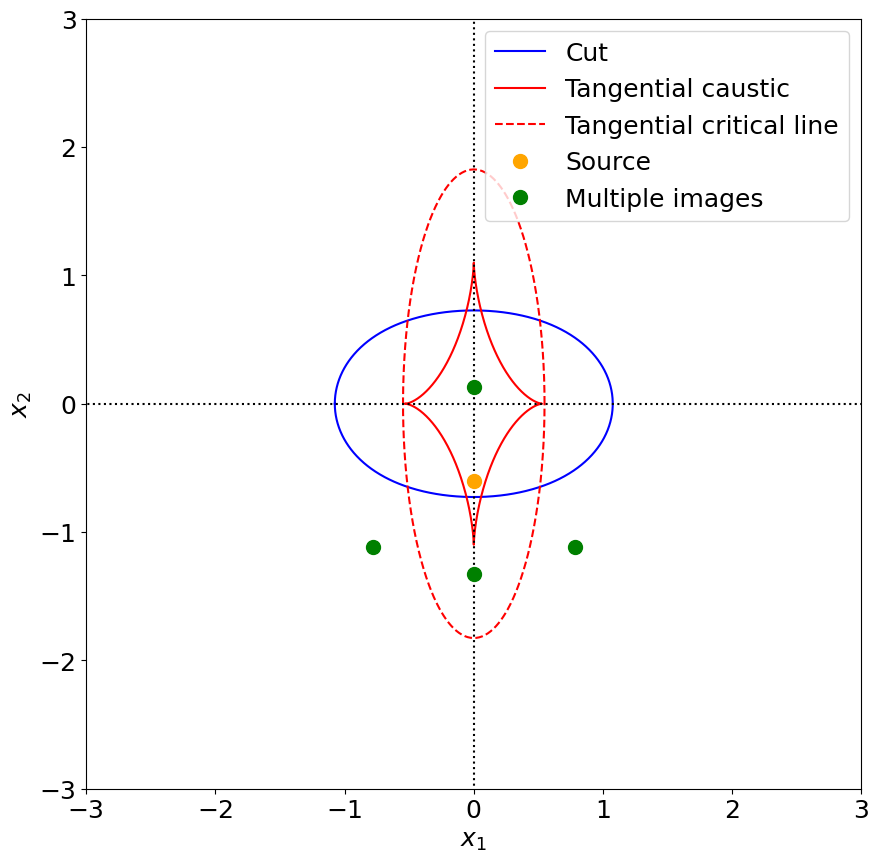
\includegraphics[width=\linewidth, keepaspectratio]{img/chapter3/sie4.png}\label{fig:sie4}}
  \end{minipage} 
  \caption[Image multiplicity for a SIE lens]{Illustration of the different image multiplicity scenarios: \protect\subref{fig:sie1} one image if the source is outside the cut, \protect\subref{fig:sie2} two images if the source is inside the cut, \protect\subref{fig:sie3} three images if the source is inside the caustic and \protect\subref{fig:sie4} four images if the source is inside both caustic and cut.}
  \label{fig:sie}
\end{figure}

\Cref{fig:sie_multiple_images} illustrate the lensing of circular sources by a SIE lens.
The upper panels illustrate the change in image geometry as the source approaches the lens center, traversing the cut and the caustic fold. Sources positioned outside the cut generate a single image, which is located in the same quadrant of the image plane as the source's projected position. Upon crossing the cut, an additional image emerges near the lens center, a consequence directly related to the cut definition. As the source moves nearer to the caustic, the central image shifts away from the lens center, appearing in the quadrant of the lens plane that is opposite to the source's projected quadrant. When the source crosses the caustic, a pair of images appear on either side of the critical line. Specifically, if the source is close to the fold in the source plane's first quadrant, the resultant images are found in the lens plane's second quadrant, adhering to the left-right mapping rule relevant to tangential critical points. As the source approaches the lens center, the resulting images form a symmetrical arrangement known as the \emph{Einstein cross}.

In the middle and bottom panels of \cref{fig:sie}, which focus on the same lens, the source moves from beyond the cut towards the lens's center, crossing through the tangential caustic cusps. At the point of caustic crossing, three images converge at the critical line, with the left-right rule once again coming into effect.

Images near the critical line are distorted tangentially, leading to the creation of \emph{gravitational arcs}. These images become elongated and tend to converge at the critical line, with the most significant gravitational arcs forming from the convergence of three images of sources located near the caustic cusps. The extent of observed distortions is influenced by the source's size in relation to the caustic. When the source is significantly larger than the caustic, the impact of the ellipticity is barely noticeable.

\begin{figure}
    \centering
    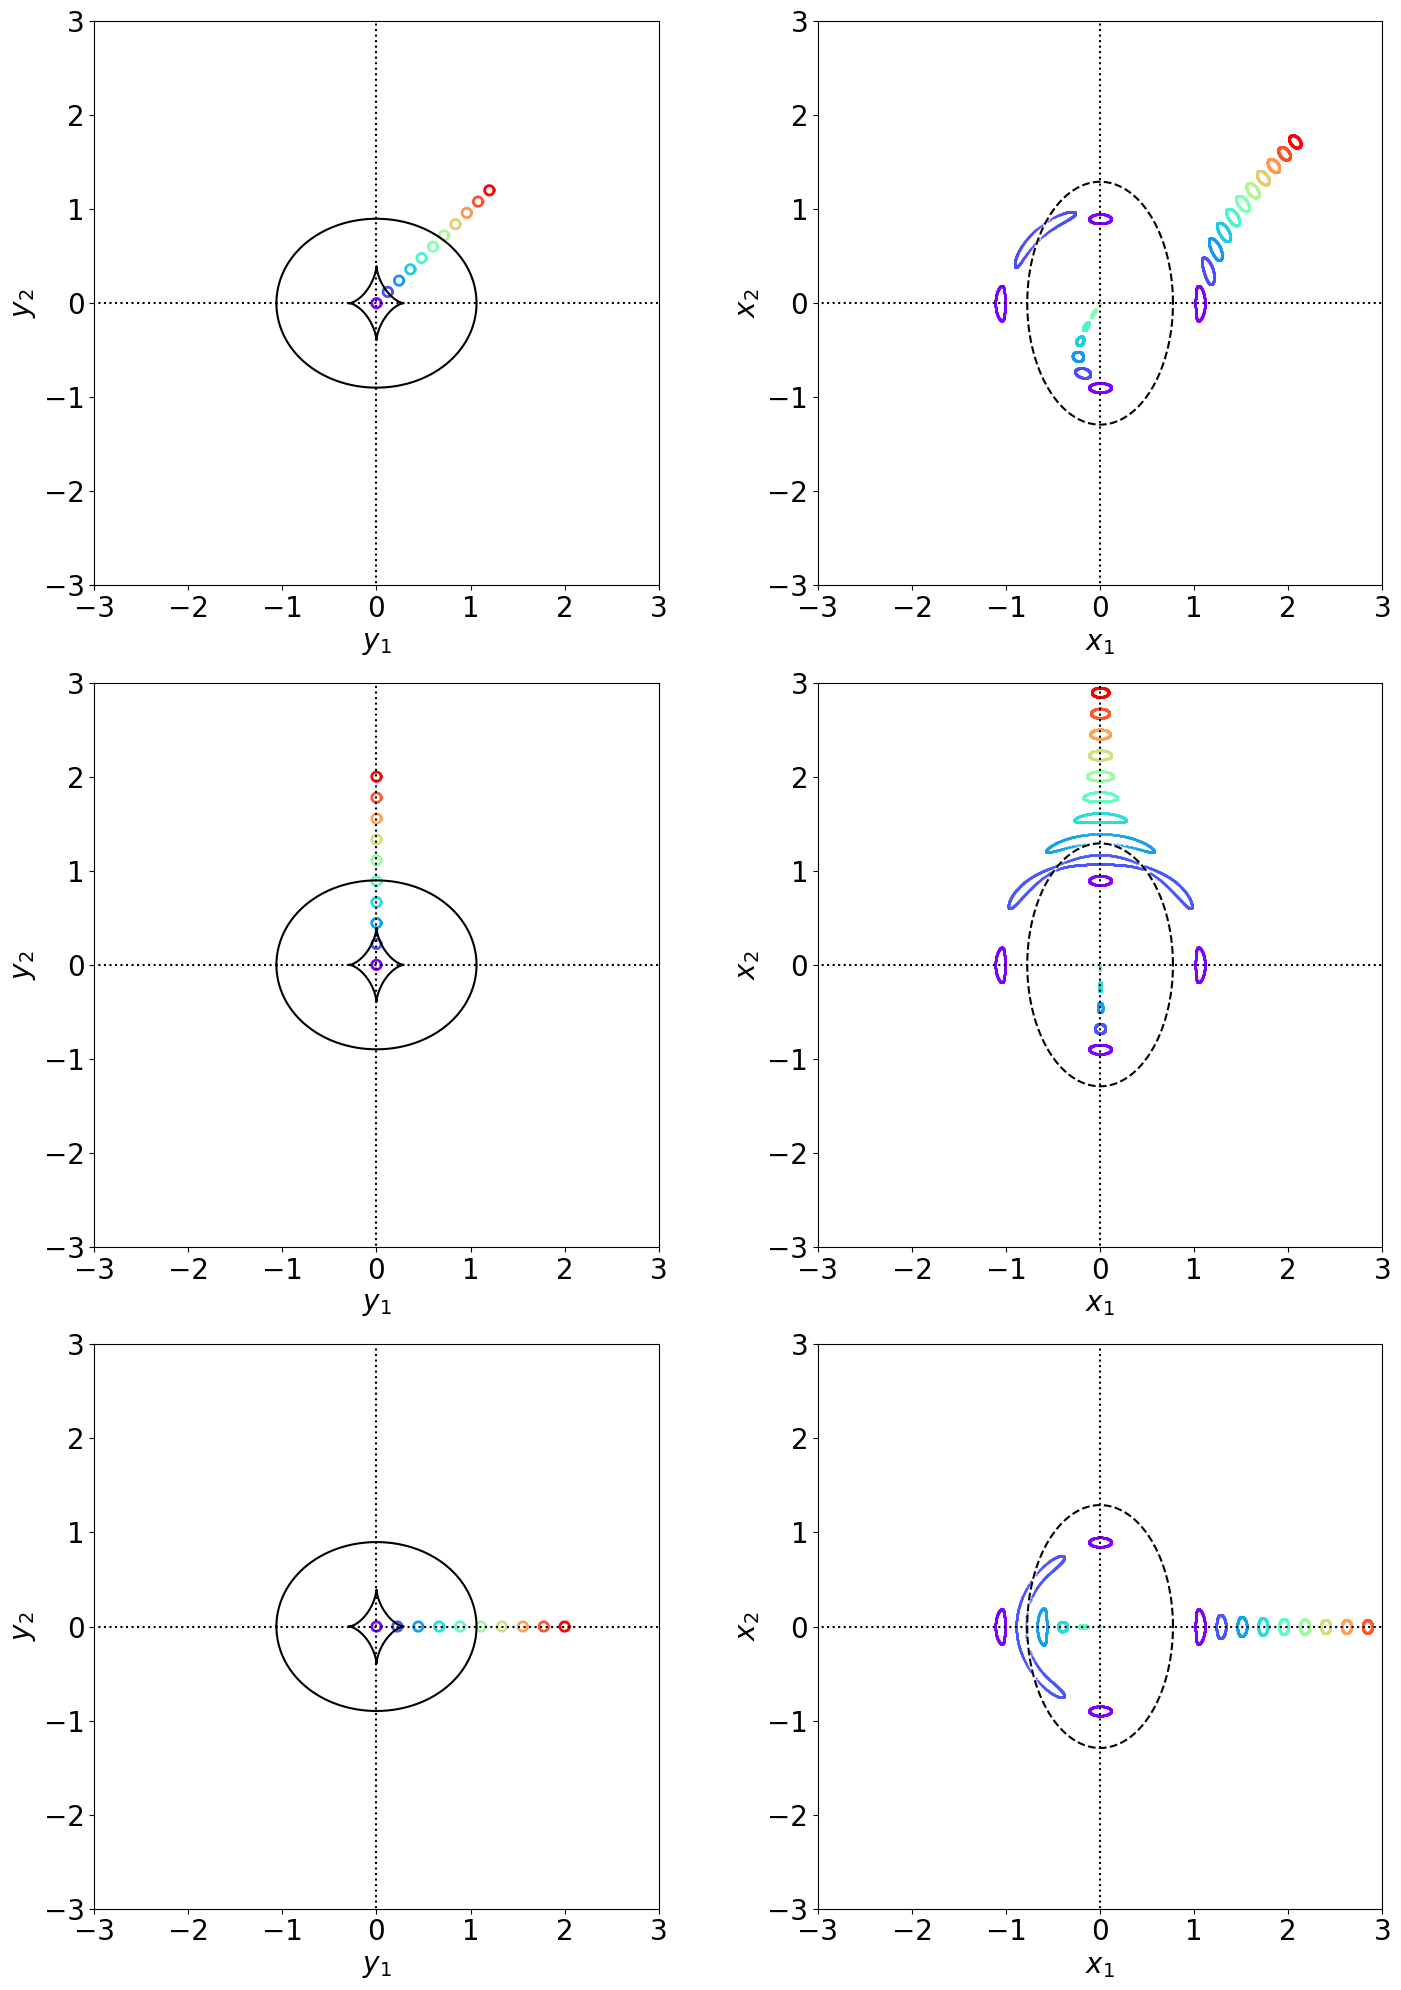
\includegraphics[width=0.9\linewidth, keepaspectratio]{img//chapter3/sie_multiple_images.png}
    \caption[Lensing of circular sources by a SIE]{Lensing of circular sources by a SIE lens with $f=0.6$. In the left panels, sources at different angular separations from the lens center. In the right panels, the correspondent multiple images.}
    \label{fig:sie_multiple_images}
\end{figure}


%%%%%%%%%%%%%%%%%%%%%%%%%%%%%%%%%%%%%%%%%%%%%%%%%%%%%%%
%%%%% Non-singular Isothermal Ellipsoid %%%%%
%%%%%%%%%%%%%%%%%%%%%%%%%%%%%%%%%%%%%%%%%%%%%%%%%%%%%%%
\subsection{Non-singular Isothermal Ellipsoid}
\label{subsec:nie}
As previously done with the SIS model, to remove the central singularity of the surface mass density, it is also possible to introduce a core for the SIE model. The resulting model, the Non-singular Isothermal Ellipsoid (NIE), has been thoroughly described by \cite{kormann_isothermal_1994,tessore_elliptical_2015}. By introducing a core radius $\x_c$ and with the usual choice of $\x_0 = \x_{0,SIS}$, the surface mass density and the convergence can be written
\begin{subequations}
\begin{align}
    \label{eq:3.42a}
    \S (\va{\x}) & = \frac{\s^2}{2 G} \frac{\sqrt{f}}{\sqrt{\x_1^2 + f^2 \x_2^2 + \x_c^2}} \,,
    \\
    \label{eq:3.42b}
    \k (\vec{x}) & = \frac{\sqrt{f}}{2 \sqrt{x_1^2 + f^2 x_2^2 + x_c^2}} \,.
\end{align}
\end{subequations}

\Cref{fig:nie} shows the different multiplicities that a NIE lens can produce of a source, depending on the value of $f$ and $x_c$. It can have two separate critical lines and caustics, only one tangential critical line and caustic, or no critical lines and caustics at all. Depending on the caustics structure, this lens can produce one, three, or five images of a source.

\begin{figure}[b!]
    \centering
    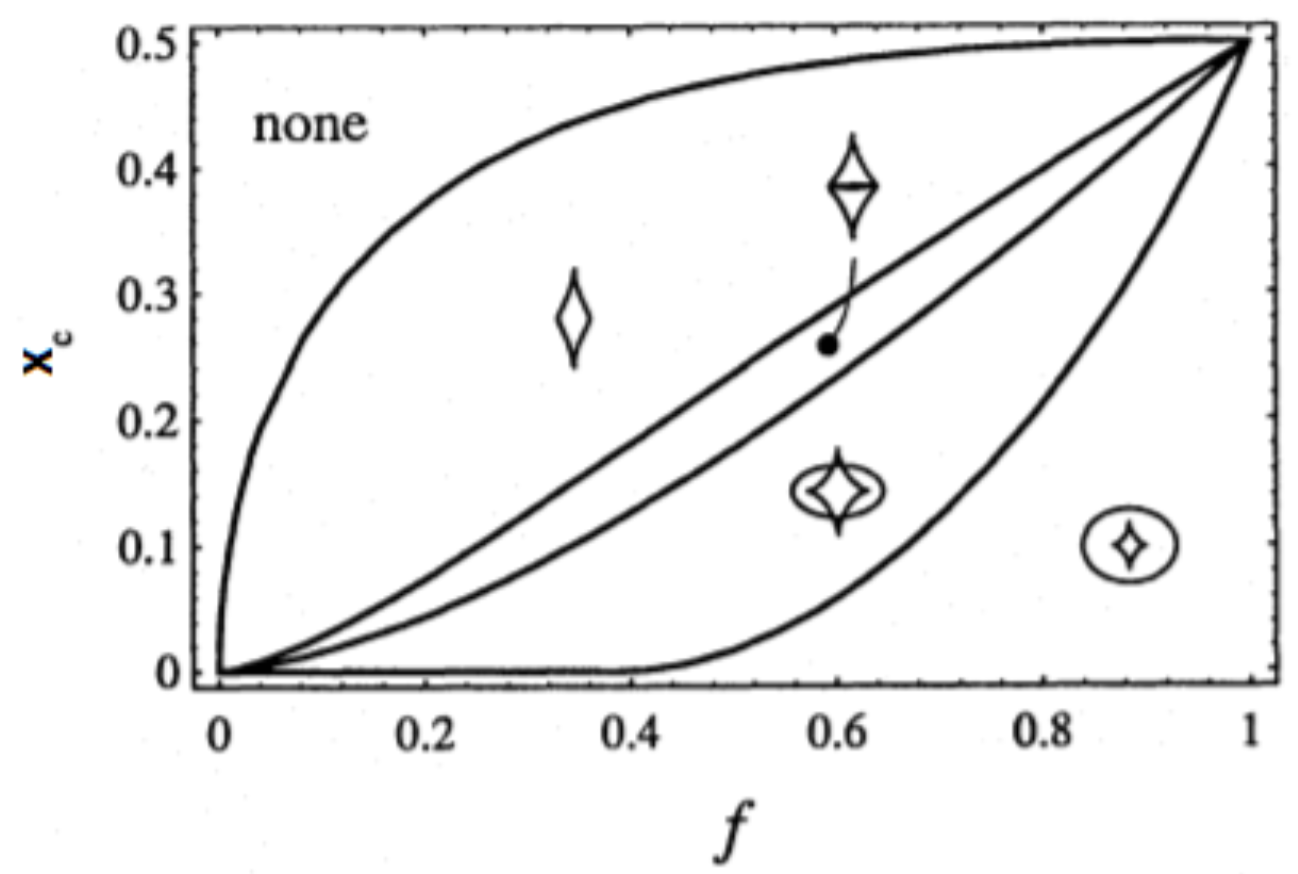
\includegraphics[width=0.9\linewidth]{img//chapter3/nie.png}
    \caption[NIE caustics topologies]{NIE caustics topologies for varying $f$ and $x_c$.\\\small{Credits: \cite{kormann_isothermal_1994}.}}
    \label{fig:nie}
\end{figure}


%%%%%%%%%%%%%%%%%%%%%%%%%%%%%%%%%%%%%%%%%%%%%%%%%%%%%%%
%%%%% External shear %%%%%
%%%%%%%%%%%%%%%%%%%%%%%%%%%%%%%%%%%%%%%%%%%%%%%%%%%%%%%
\subsection{External shear}
\label{subsec:ext_shear}
When analyzing a gravitational lens located in a densely populated environment, it becomes crucial to consider the gravitational influence of the surrounding mass distributions. A usual approach to encapsulate the effects of this environment is to employ the concept of an external shear field. This field is characterized through a potential that allows the quantification of the environmental impact on the lensing effects observed. The external shear field effectively models the tidal forces exerted by nearby mass distributions that are not directly part of the lens, but nevertheless influence the path of light rays passing near the lens.

The presence of the external shear field can be modeled by means of a potential $\P_\g$, such that
\begin{equation}
\begin{aligned}
    \label{eq:3.43}
    \g_1 & = \frac{1}{2} (\P_{11} - \P_{22}) = \mathrm{const.}
    \\
    \g_2 & = \P_{12} = \mathrm{const.}
    \\
    \k & = \frac{1}{2} (\P_{11} + \P_{22}) = \mathrm{const.}
\end{aligned}
\end{equation}

This means that $\P_{11}$ and $\P_{22}$ must be both constants and the potential is quadratic:
\be
\label{eq:3.44}
\P_\g (\vec{x}) = C x_1^2 + C^\prime x_2^2 + D x_1 x_2 + E \,.
\ee

Differentiating \cref{eq:3.44} and substituting into \cref{eq:3.43}:
\begin{equation}
\begin{aligned}
    \label{eq:3.45}
    \g_1 & = \frac{1}{2} (\P_{11} - \P_{22}) = C - C^\prime \,,
    \\
    \g_2 & = \P_{12} = D \,,
    \\
    \k & = \frac{1}{2} (\P_{11} + \P_{22}) = C + C^\prime \,.
\end{aligned}
\end{equation}

At this point, it is possible to distinguish two cases:
\begin{itemize}
    \item $\k = 0$ if the external perturbation does not contribute to the convergence, which means $C = C^\prime = \g_1 / 2$ and
    \be
    \label{eq:3.46}
    \P_\g = \frac{\g_1}{2} (x_1^2 - x_2^2) + \g_2 x_1 x_2 \,.
    \ee
    \item $\g_1, \g_2 = 0$ if the lens is embedded in a sheet of constant surface mass density producing no shear (no privileged directions); in this case the external convergence potential is
    \be
    \label{eq:3.47}
    \P_\k = \frac{\k}{2} x^2 \,,
    \ee
    and can be inserted into the lens equation
    \be
    \label{eq:3.48}
    \va{\a} (\vec{x}) = \va{\nabla} \P_\k (\vec{x}) = \k \vec{x} \,,
    \ee
    to obtain
    \be
    \label{eq:3.49}
    \vec{y} = \vec{x} - \va{\a} (\vec{x}) = \vec{x} (1 - \k) \,.
    \ee

    If $\k = 1$, this sheet acts as a perfectly convergent lens, mapping every position $\vec{x}$ on the lens plane to the same point $y=0$.
\end{itemize}


% *************************************************************
%%%%% CHAPTER 4: OPTIMIZATION ALGORITHMS %%%%%
\cleardoublepage
\chapter[Algorithms]{Algorithms}
\label{chap:algorithms}

Building on the foundational understanding of gravitational lensing and its computational challenges, a critical aspect of modern astrophysical research involves the optimization of parametric functions to model the complex phenomena of the Universe accurately. This optimization is essential in gravitational lensing studies, where precise models of the mass distribution within lensing objects are paramount for interpreting the observed lensing effects. The optimization process often requires navigating a high-dimensional parameter space to find the best-fit parameters that reconcile theoretical models with observational data, a task that can be computationally intensive and algorithmically complex.

In this context, the advent of frameworks such as PyTorch\footnote{\url{https://pytorch.org}} \citep{paszke_pytorch_2019} and TensorFlow\footnote{\url{https://www.tensorflow.org}} \citep{abadi_tensorflow_2016} represents a significant leap forward for astrophysical research. These open-source libraries, primarily developed for deep learning applications, offer powerful tools for automatic differentiation, a technique that facilitates the calculation of gradients automatically, a cornerstone for any optimization algorithm. The ability of PyTorch and TensorFlow to efficiently compute derivatives of highly complex, nested functions makes them exceptionally well suited for optimizing parametric models in gravitational lensing studies.

Moreover, PyTorch and TensorFlow are designed to exploit the capabilities of modern computing hardware, including GPUs and TPUs, enabling the parallel processing of large datasets and the acceleration of computational tasks. This feature is particularly beneficial for gravitational lensing research, where handling large amounts of observational data and running complex simulations is commonplace. Using the computational power offered by these frameworks, one can significantly reduce the time required for model optimization and data analysis, thus enhancing the efficiency of the investigations.

% *************************************************************
%%%%% SECTION 4.1: DIFFERENTIABLE PROGRAMMING %%%%%
%%%%%%%%%%%%%%%%%%%%%%%%%%%%%%%%%%%%%%%%%%%%%%%%%%%%%%%
%%%%% Sec: Differentiable programming %%%%%
%%%%%%%%%%%%%%%%%%%%%%%%%%%%%%%%%%%%%%%%%%%%%%%%%%%%%%%
\section{Differentiable programming}
\label{sec:diff_prog}

Differentiable programming is an advanced computational paradigm that unites traditional programming concepts with the principles of differentiation, a fundamental concept in calculus. This approach extends the idea of computing derivatives to entire programs, enabling the automatic calculation of gradients of program outputs with respect to inputs. Differentiable programming is particularly powerful in the context of optimization, machine learning, and artificial intelligence, where it facilitates efficient parameter tuning to minimize or maximize some objective function.
Methods for computing derivatives in computer programs can be classified into four categories (see \cref{fig:diff_methods}):
\begin{enumerate}
    \item manually working out derivatives and coding them;
    \item \textbf{numerical differentiation}, involves approximating the derivative of a function using values of the original function evaluated at some sample points \citep{burden_numerical_2016}. In its simplest form, it is based on the limit definition of a derivative. It is quite simple to implement and apply to a wide range of problems, especially when dealing with data-driven models or functions that lack a clear analytical representation. Its effectiveness diminishes in high-dimensional settings, where the complexity and computational demands increase exponentially, highlighting the method's limitations in handling complex, multi-variable functions efficiently;
    \item \textbf{symbolic differentiation}, which refers to the automatic process of finding derivatives using the rules of differentiation to obtain an exact symbolic expression for the derivative of a given function \citep{grabmeier_computer_2003}. This method works similarly to how humans perform differentiation ``by hand'', manipulating symbols according to mathematical laws;
    \item \textbf{automatic differentiation} (AD), also called algorithmic differentiation,is a method that computes the derivative of a function efficiently and accurately by systematically applying the chain rule of calculus to the sequence of elementary operations (additions, multiplications, trigonometric functions, etc.) that constitute a computer program. All numerical computations are ultimately compositions of a finite set of elementary operations for which derivatives are known \citep{verma_introduction_2000,griewank_evaluating_2008}, and combining the derivatives of the constituent operations through the chain rule of calculus\footnote{The derivative of the composition of two (or more) differentiable functions $f$ and $g$ can be expressed in terms of the derivatives of the single functions $f$ and $g$. If $h (x) = f(g(x))$, then $h^\prime(x) = f^\prime(g(x)) g^\prime(x)$.} gives the derivative of the overall composition. AD is not an approximation like numerical differentiation, but rather computes derivatives to machine precision.
\end{enumerate}
\newpage
In particular, differentiable programming refers to using automatic differentiation in some way that allows a program to optimize its parameters to improve on some task. It only has three requirements:
\begin{enumerate}
    \item a parameterized function/model to be optimized;
    \item (automatic) differentiability of the object to be optimized;
    \item a function suitable to measure the performance of the model.
\end{enumerate}

The process of optimizing a model in the field of differentiable programming is often called \emph{training}.
In the subsequent portion of this section, a comprehensive overview of automatic differentiation and its role in the training process will be provided. This will be followed by an in-depth exposition of the process itself.

\begin{figure}
    \centering
    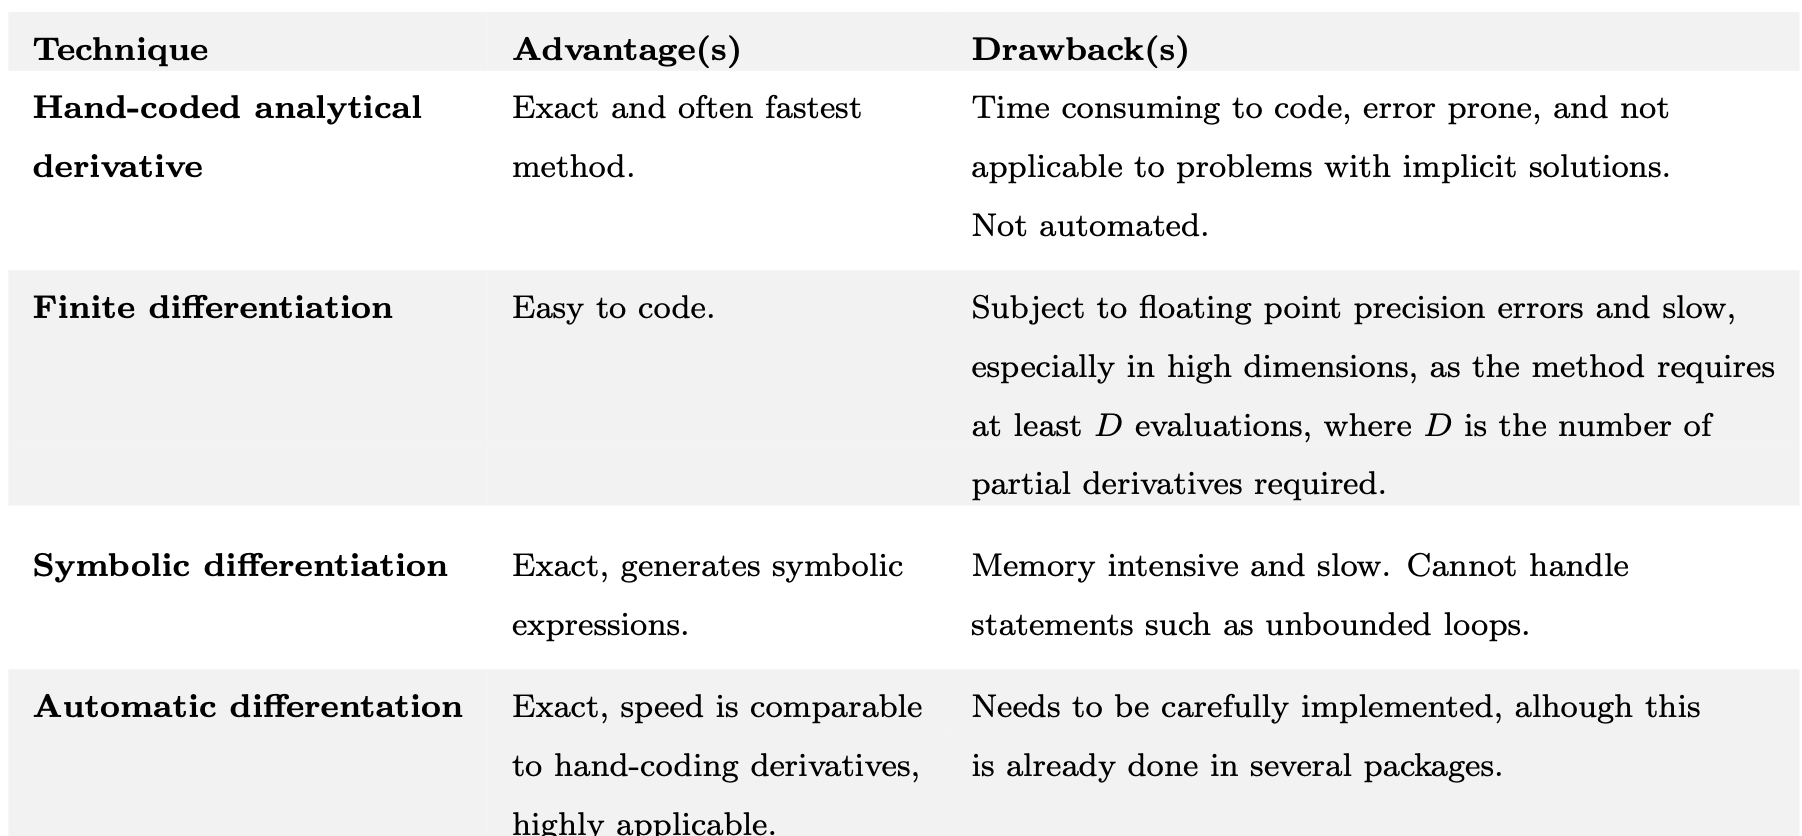
\includegraphics[width=\linewidth, keepaspectratio]{img//chapter4/diff_methods.png}
    \caption[Summary of techniques to calculate derivatives]{Summary of techniques to calculate derivatives.\\\small{Credits: \cite{margossian_review_2019}.}}
    \label{fig:diff_methods}
\end{figure}


%%%%%%%%%%%%%%%%%%%%%%%%%%%%%%%%%%%%%%%%%%%%%%%%%%%%%%%
%%%%% SubSec: Automatic differentiation %%%%%
%%%%%%%%%%%%%%%%%%%%%%%%%%%%%%%%%%%%%%%%%%%%%%%%%%%%%%%
\subsection{Automatic differentiation}
\label{subsec:automatic_differentiation}


%%%%%%%%%%%%%%%%%%%%%%%%%%%%%%%%%%%%%%%%%%%%%%%%%%%%%%%
%%%%% SubSubSec: Computational graph %%%%%
%%%%%%%%%%%%%%%%%%%%%%%%%%%%%%%%%%%%%%%%%%%%%%%%%%%%%%%
\subsubsection{Computational graph}
\label{subsubsec:computational_graph}
As already stated, automatic differentiation operates on the fundamental principle that complex functions can be decomposed into a series of elementary arithmetic operations. Given a target composite function $f (x) = h \circ g(x) = h(g(x))$, with $x \in \mathbb{R}^n$, $g : \mathbb{R}^n \rightarrow \mathbb{R}^k$, and $h : \mathbb{R}^k \rightarrow \mathbb{R}^m$, applying the chain rule and elementary matrix multiplication, the corresponding Jacobian matrix\footnote{The Jacobian matrix of a vector-valued function of several variables is the matrix of all its first-order partial derivatives.} $J$ is thus:
\be
\label{eq:4.1}
J = J_{h \circ g} = J_h (g(x)) \cdot J_g (x) \,,
\ee
with $(i,j)^{th}$ element:
\be
\label{eq:4.2}
J_{ij} = \frac{\partial f_i}{\partial x_j} = \frac{\partial h_i}{\partial g_1} \frac{\partial g_1}{\partial x_j} + \frac{\partial h_i}{\partial g_2} \frac{\partial g_2}{\partial x_j} + \ldots + \frac{\partial h_i}{\partial g_k} \frac{\partial g_k}{\partial x_j} \,.
\ee

More generally, if $f$ is the composite expression of $L$ functions
\be
\label{eq:4.3}
f = f^L \circ f^{L-1} \circ \ldots \circ f^1 \,,
\ee
the corresponding Jacobian matrix will be
\be
\label{eq:4.4}
J = J_L \cdot J_{L-1} \cdot \ldots \cdot J_1 \,.
\ee
Hence, given a complex function $f$, it is possible to break down the action of the Jacobian matrix on a vector into simple components.
So, following \cite{griewank_evaluating_2008} notation, a function $f : \mathbb{R}^n \rightarrow \mathbb{R}^m$ can be constructed using intermediate variables $v_i$ such that
\begin{itemize}
    \item variables $v_{i-n} = x_i$, $i = 1, \ldots, n$ are the input variables,
    \item variables $v_{i}$, $i = 1, \ldots, l$ are the intermediate variables,
    \item variables $y_{m-i} = v_{l-i}$, $i = m-1, \ldots, 0$ are the output variables.
\end{itemize}
The representation of all the elementary operations that take place to construct a certain function $f$ is called the \emph{evaluation trace}, which can also be pictured as a \emph{computational graph} \citep{bauer_computational_1974}, useful for visualizing the dependency relations between intermediate variables. \Cref{fig:computational_graph} shows the computation graph for an example function $f : \mathbb{R}^2 \rightarrow \mathbb{R}$: 
\be
\label{eq:4.5}
f(x_1, x_2) = \ln{(x_1)} + x_1 x_2 - \sin{(x_2)} \,.
\ee

\begin{figure}
    \centering
    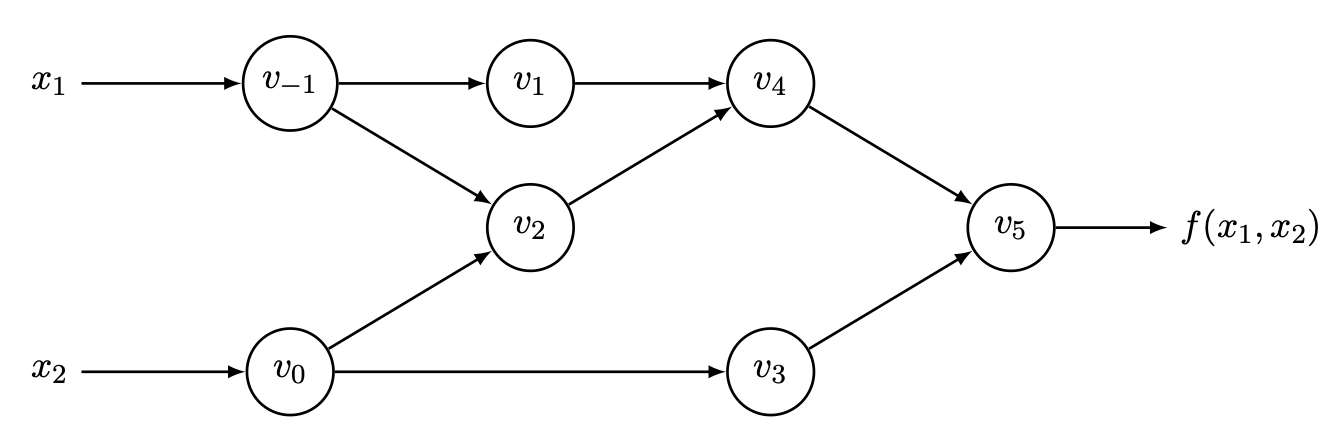
\includegraphics[width=0.9\linewidth, keepaspectratio]{img//chapter4/computational_graph.png}
    \caption[Example of computational graph]{Computational graph of the example $f(x_1, x_2) = \ln{(x_1)} + x_1 x_2 - \sin{(x_2)}$.\\\small{Credits: \cite{baydin_automatic_2018}.}}
    \label{fig:computational_graph}
\end{figure}

Given the computational graph of all elementary operations, AD can be implemented in two main modes: \emph{forward} accumulation mode and \emph{reverse} accumulation mode (backward mode).


%%%%%%%%%%%%%%%%%%%%%%%%%%%%%%%%%%%%%%%%%%%%%%%%%%%%%%%
%%%%% SubSubSec: Forward mode %%%%%
%%%%%%%%%%%%%%%%%%%%%%%%%%%%%%%%%%%%%%%%%%%%%%%%%%%%%%%
\subsubsection{Forward mode}
\label{subsubsec:forward_mode}
Automatic differentiation in forward accumulation mode (or \emph{tangent linear} mode) is the conceptually most simple type. The differentiation process is aligned with the function evaluation itself. Starting from the inputs, the program computes both the function's value and its derivative step by step through the computation graph. For each elementary operation, the forward mode calculates the derivative of the output with respect to the inputs, carrying these derivatives (or ``tangents'') forward through the computation graph.

Considering as an example the evaluation trace of the function defined in \cref{eq:4.5} (left-hand side of \cref{fig:forward_trace}), for computing the derivative of $f$ with respect to $x_1$, the first step is to associate with each intermediate variable $v_i$ a derivative
\be
\label{eq:4.6}
\Dot{v}_i = \frac{\partial v_i}{\partial x_1}.
\ee

Applying then the chain rule to each elementary operation in the forward primal trace, the corresponding tangent (derivative) trace is generated (right-hand side of \cref{fig:forward_trace}), until the required derivative in the final variable $\Dot{v}_5 = \frac{\partial y}{\partial x_1}$ is obtained.

Generalizing this procedure to a function $f : \mathbb{R}^n \rightarrow \mathbb{R}^m$, each forward pass of AD provides one column of the Jacobian matrix (\ie the partial derivatives of all output variables with respect to one input variable).
Thus, the complete Jacobian can be computed in $n$ evaluations. For this reason, forward AD is efficient and straightforward especially for functions $f : \mathbb{R} \rightarrow \mathbb{R}^m$, for which all derivatives can be computed with just one forward pass.

In general, for functions with many inputs $f : \mathbb{R}^n \rightarrow \mathbb{R}^m$ where $n \gg m$, the reverse accumulation mode of AD is preferred.

\begin{figure}
    \centering
    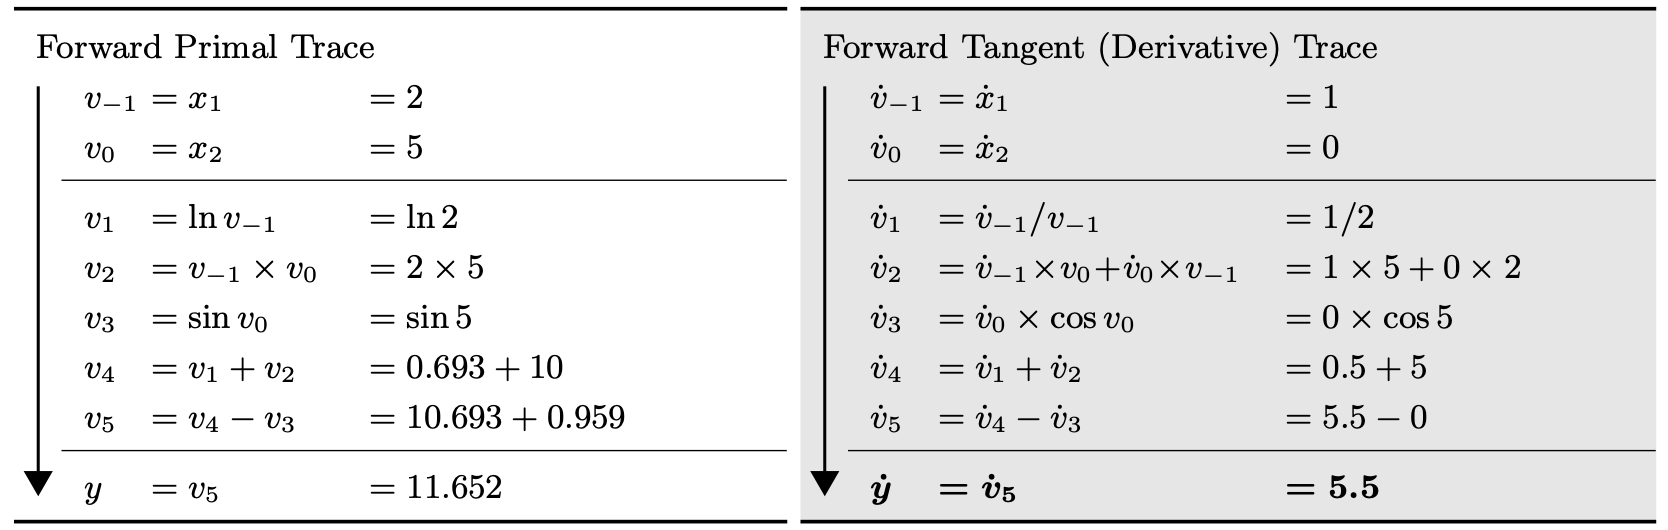
\includegraphics[width=\linewidth]{img//chapter4/forward_trace.png}
    \caption[Forward mode AD example]{Forward mode AD example for $f(x_1, x_2) = \ln{(x_1)} + x_1 x_2 - \sin{(x_2)}$, evaluated at $(x_1, x_2) = (2, 5)$ by setting $\Dot{x}_1 = 1$. The original forward evaluation of the primals on the left is augmented by the tangent operations on the right, where each line complements the original directly to its left.\\\small{Credits: \cite{baydin_automatic_2018}.}}
    \label{fig:forward_trace}
\end{figure}


%%%%%%%%%%%%%%%%%%%%%%%%%%%%%%%%%%%%%%%%%%%%%%%%%%%%%%%
%%%%% SubSubSec: Reverse mode %%%%%
%%%%%%%%%%%%%%%%%%%%%%%%%%%%%%%%%%%%%%%%%%%%%%%%%%%%%%%
\subsubsection{Reverse mode}
\label{subsubsec:reverse_mode}
AD in reverse accumulation mode (or \emph{adjoint} or \emph{cotangent linear} mode) \citep{griewank_numerical_2012} corresponds to a generalized backpropagation algorithm, in that it propagates derivatives backward from a given output. This is done by complementing each variable $v_i$ with an adjoint
\be
\label{eq:4.7}
\overline{v}_i = \frac{\partial y_j}{\partial v_i} \,,
\ee
which represents the sensitivity of a considered output $y_j$ with respect to changes in $v_i$.

In reverse mode AD, derivatives are computed in the second of a two-phase process. In the first phase, the original function code is run forward, creating intermediate variables $v_i$ and recording the dependencies in the computational graph. In the second phase, derivatives are calculated by propagating adjoints $\overline{v}_i$ in reverse, from outputs to inputs. The reverse mode AD for the example function of \cref{eq:4.5} is shown in \cref{fig:reverse_trace}.

An important advantage of the reverse mode is that it is significantly less costly to evaluate (in terms of operation count) than the forward mode for functions with a large number of inputs. In the extreme case of $f : \mathbb{R}^n \rightarrow \mathbb{R}$, only one application of the reverse
mode is sufficient to compute the full gradient, compared with the $n$ passes of the forward mode needed to populate the same. Because the optimization of astrophysical and gravitational lensing parametric functions usually involves the gradient of a scalar-valued objective with respect to a (large) number of parameters, this establishes the reverse mode, as opposed to the forward mode, as the mainstay technique in the form of the backpropagation algorithm \citep{schmidhuber_deep_2015}.

\begin{figure}
    \centering
    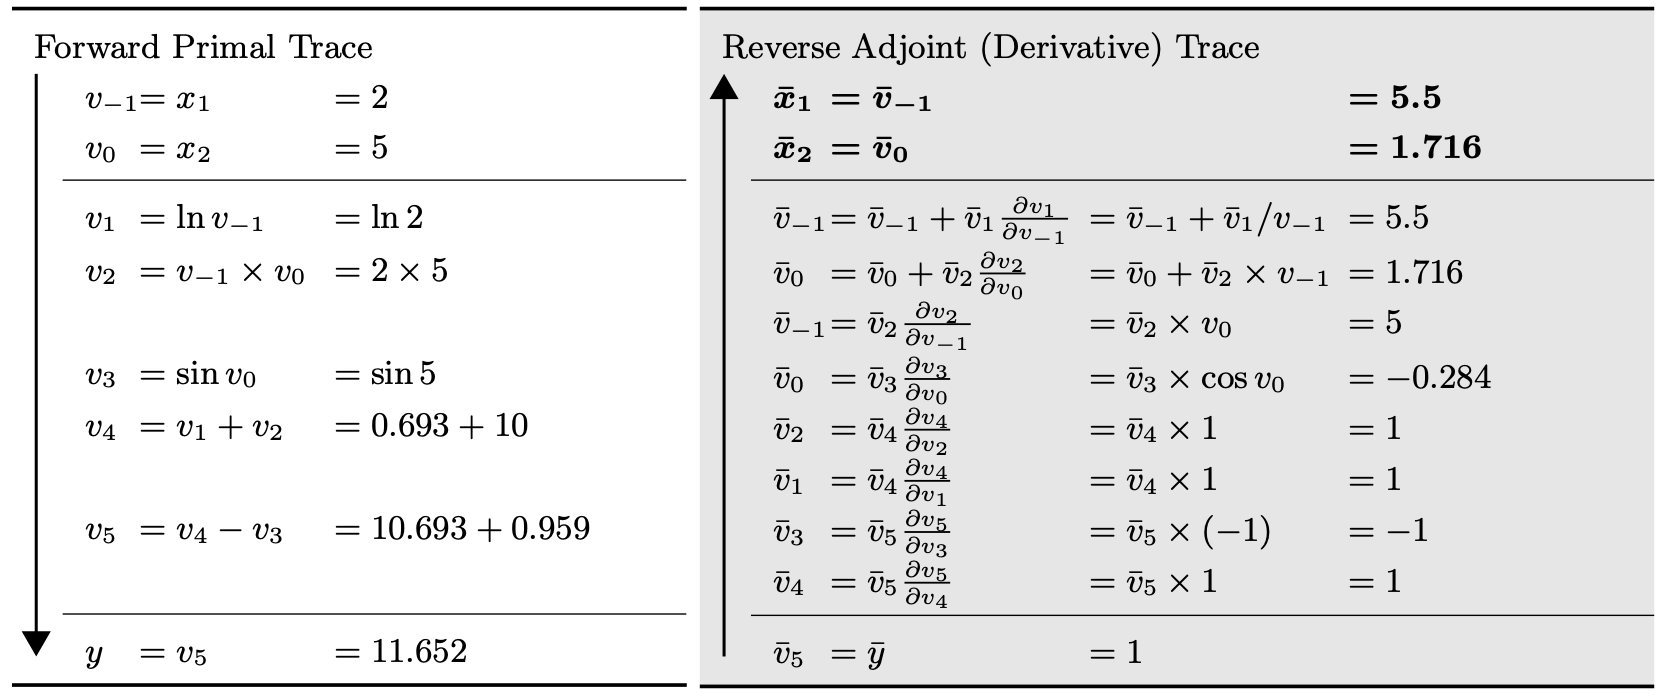
\includegraphics[width=0.9\linewidth, keepaspectratio]{img//chapter4/reverse_trace.png}
    \caption[Reverse mode AD example]{Reverse mode AD example for $f(x_1, x_2) = \ln{(x_1)} + x_1 x_2 - \sin{(x_2)}$, evaluated at $(x_1, x_2) = (2, 5)$. After forward evaluation of the primals on the left, adjoint operations on the right are evaluated in reverse.\\\small{Credits: \cite{baydin_automatic_2018}.}}
    \label{fig:reverse_trace}
\end{figure}


%%%%%%%%%%%%%%%%%%%%%%%%%%%%%%%%%%%%%%%%%%%%%%%%%%%%%%%
%%%%% SubSec: Backpropagation algorithm %%%%%
%%%%%%%%%%%%%%%%%%%%%%%%%%%%%%%%%%%%%%%%%%%%%%%%%%%%%%%
\subsection{Backpropagation algorithm}
\label{subsec:backpropagation_algorithm}
The backpropagation algorithm is the cornerstone of neural network training \citep{rumelhart_learning_1986,montavon_efficient_2012}, mainly used to minimize the error by adjusting the weights of the connections in the network. However, when it comes to a model optimization problem outside the realm of neural networks, such as training parametric models, the concept of backpropagation refers to the method of computing gradients efficiently using reverse mode AD.

The training process (or better, the training loop) is characterized by a sequence of operations performed recursively. The optimization itself is performed by an \emph{optimizer} which operates by tweaking the model parameters in a certain way, with the purpose of minimizing a \emph{loss} function, which quantifies the difference between the predicted outputs of the model and the actual target/observed values. 
The main algorithm that allows for this optimization is the so-called \emph{gradient descent.}


%%%%%%%%%%%%%%%%%%%%%%%%%%%%%%%%%%%%%%%%%%%%%%%%%%%%%%%
%%%%% SubSubSec: Loss function %%%%%
%%%%%%%%%%%%%%%%%%%%%%%%%%%%%%%%%%%%%%%%%%%%%%%%%%%%%%%
\subsubsection{Loss function}
\label{subsubsec:loss_func}
As mentioned above, the loss function provides a measure of the performance of the model. The goal of optimization is to adjust the model parameters in a way that minimizes the loss function. The choice of loss function depends on the specific problem and the model.
Common examples include the Mean Squared Error (MSE) for regression problems
\be
\label{eq:4.8}
\mathrm{MSE} = \frac{1}{n} \sum_{i=1}^n (y_i - \hat{y}_i)^2 \,,
\ee
where $y_i$ and $\hat{y_i}$ are the observed and predicted values, respectively, and the Cross-Entropy Loss for classification problems. 

A common loss function used in the optimization of the gravitational lensing models is the chi-squared ($\chi^2$) statistic, which is the sum of squared differences between observed ($y$) and model-predicted ($\hat{y}$) values, normalized by uncertainties ($\s$) in observations:
\be
\label{eq:4.9}
\chi^2 = \sum_{i=1}^n \bp{\frac{y_i - \hat{y}_i}{\s_i}}^2 \,.
\ee

The loss function is a crucial component because it guides the training process by indicating the direction in which the model parameters should be adjusted. 


%%%%%%%%%%%%%%%%%%%%%%%%%%%%%%%%%%%%%%%%%%%%%%%%%%%%%%%
%%%%% SubSubSec: Gradient descent %%%%%
%%%%%%%%%%%%%%%%%%%%%%%%%%%%%%%%%%%%%%%%%%%%%%%%%%%%%%%
\subsubsection{Gradient descent}
\label{subsubsec:grad_descent}
Gradient-based optimization is one of the pillars of machine learning \citep{bottou_optimization_2018} and is one of the most common optimization algorithms for parametric functions. It is used to find the values of the parameters of a function that decrease the loss function as much as possible \citep{chandra_gradient_2022,ruder_overview_2016}. Given a loss function $f : \mathbb{R}^n \rightarrow \mathbb {R}$, and starting from random initial values of the parameters $\vec{\t}$, classical gradient descent has the objective of finding (local) minima
\be
\label{eq:4.10}
\hat{\vec{\t}} = \argmin_{\vec{\t}} f(\vec{\t}) \,,
\ee
which means finding the set of parameters $\hat{\vec{\t}} \in \mathbb{R}^n$ that minimizes the loss function, as shown in \cref{fig:grad_descent}. In complex models, $f$ might have multiple local minima, and the algorithm seeks to find at least one of these, via updates of the form
\be
\label{eq:4.11}
\D \vec{\t} = - \eta \va{\nabla}_{\va{\t}} f
\ee
where $\eta > 0$ is the so-called step size, also known as \emph{learning rate}, which determines how big a step is taken in the direction opposite to the gradient. Choosing the appropriate $\eta$ is crucial; too small, and the algorithm converges slowly, too large, and it can overshoot the minimum or diverge (see \cref{fig:lr_small_high}). Gradient-based methods make use of the fact that $f$ decreases the steepest moving in the direction of the negative gradient. The convergence rate of gradient-based methods is generally improved by adaptive step size techniques that adjust step size $\eta$ on each iteration \citep{duchi_adaptive_2011,schaul_no_2013,kingma_adam_2017}.

\begin{figure}
  \centering
  \subfloat[]{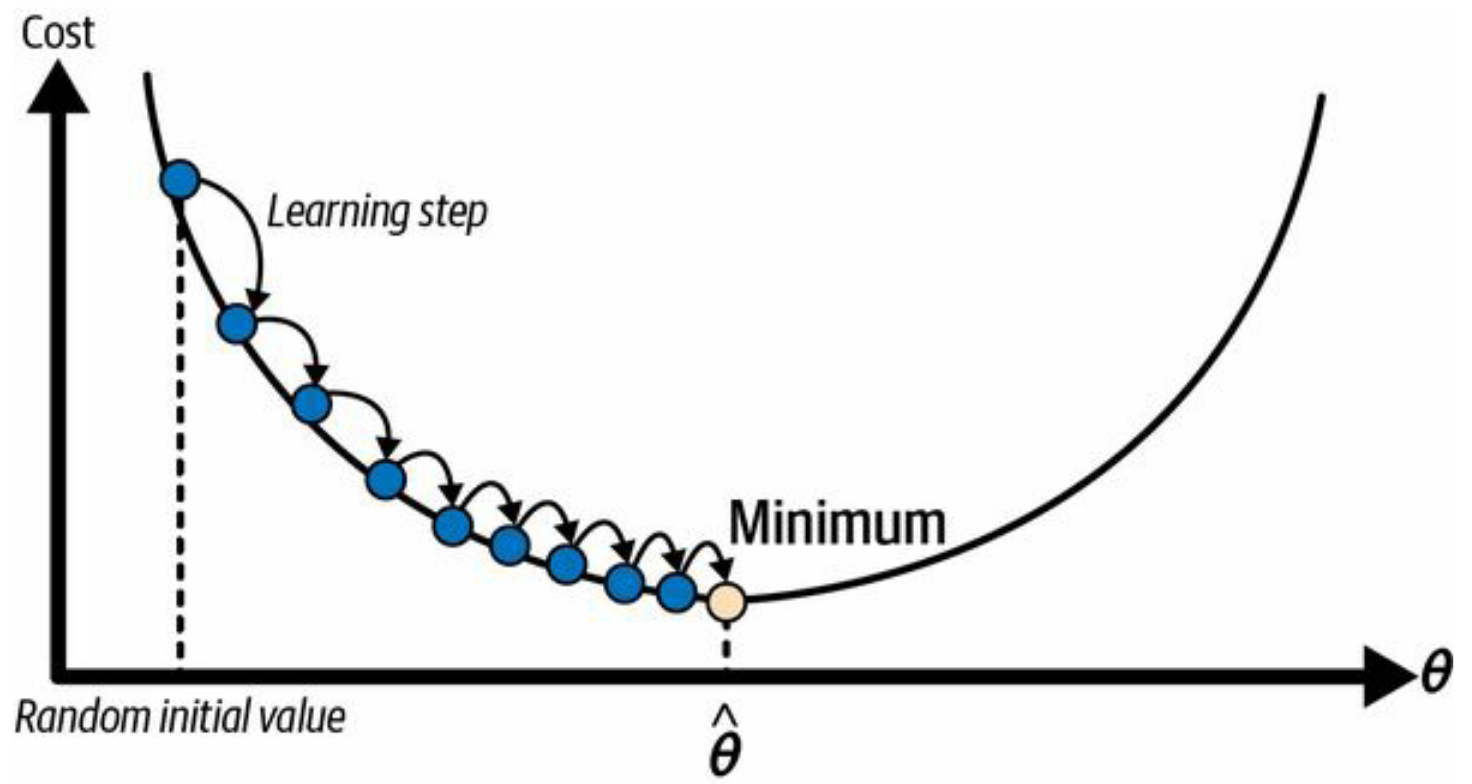
\includegraphics[width=0.5\linewidth, keepaspectratio]{img//chapter4/gradient_descent.png}\label{fig:grad_descent1d}}
  \hfill
  \subfloat[]{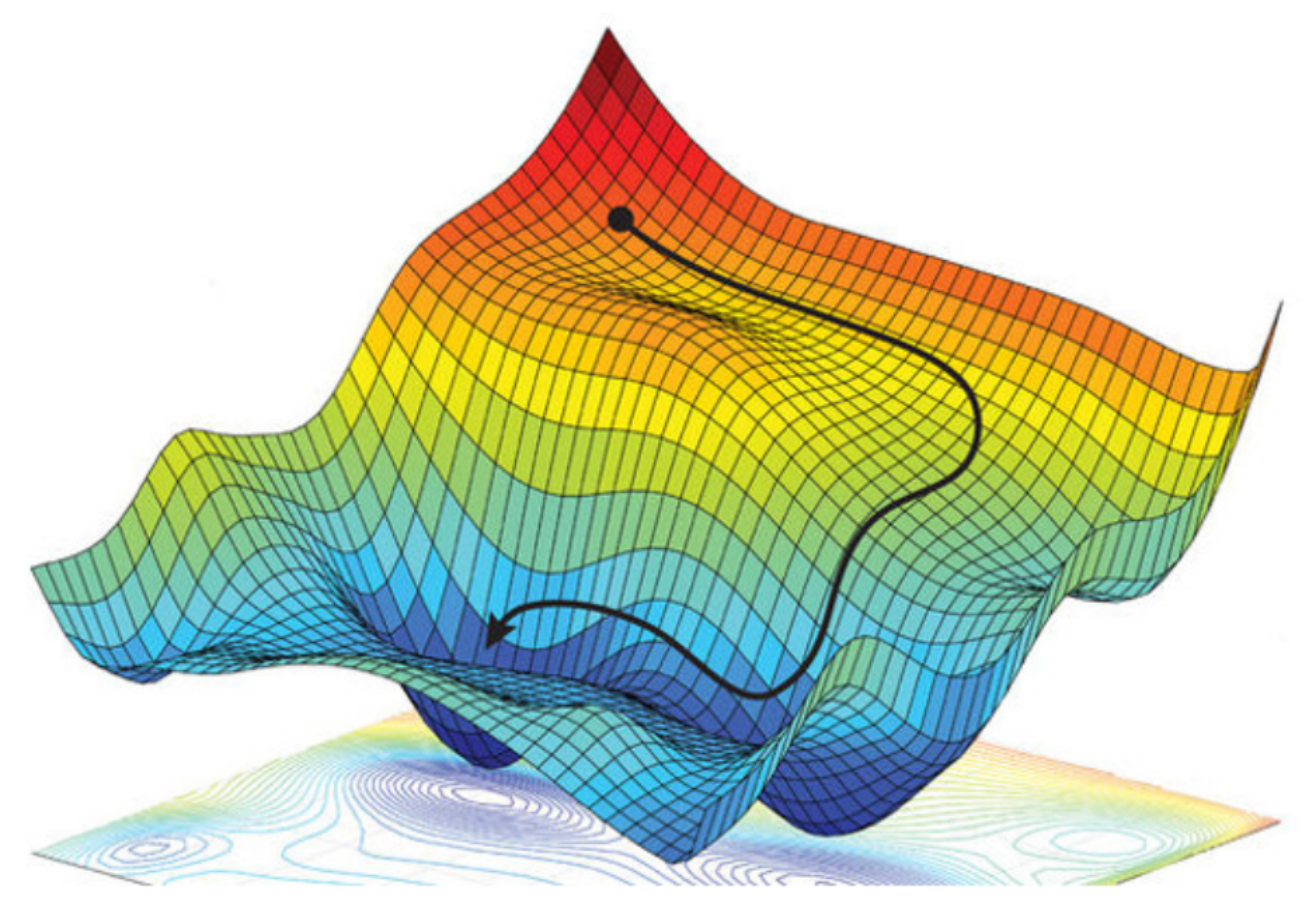
\includegraphics[width=0.5\linewidth, keepaspectratio]{img//chapter4/gradient_descent2d.png}\label{fig:grad_descent2d}}
  \caption[One/two-dimensional gradient descents]{Examples of gradient descents for a \protect\subref{fig:grad_descent1d} one-dimensional loss function and for a \protect\subref{fig:grad_descent2d} two-dimensional one.\\\small{Credits: \cite{geron_hands-machine_2019,amini_spatial_2018}.}}
  \label{fig:grad_descent}
\end{figure}

\begin{figure}
  \centering
  \subfloat[]{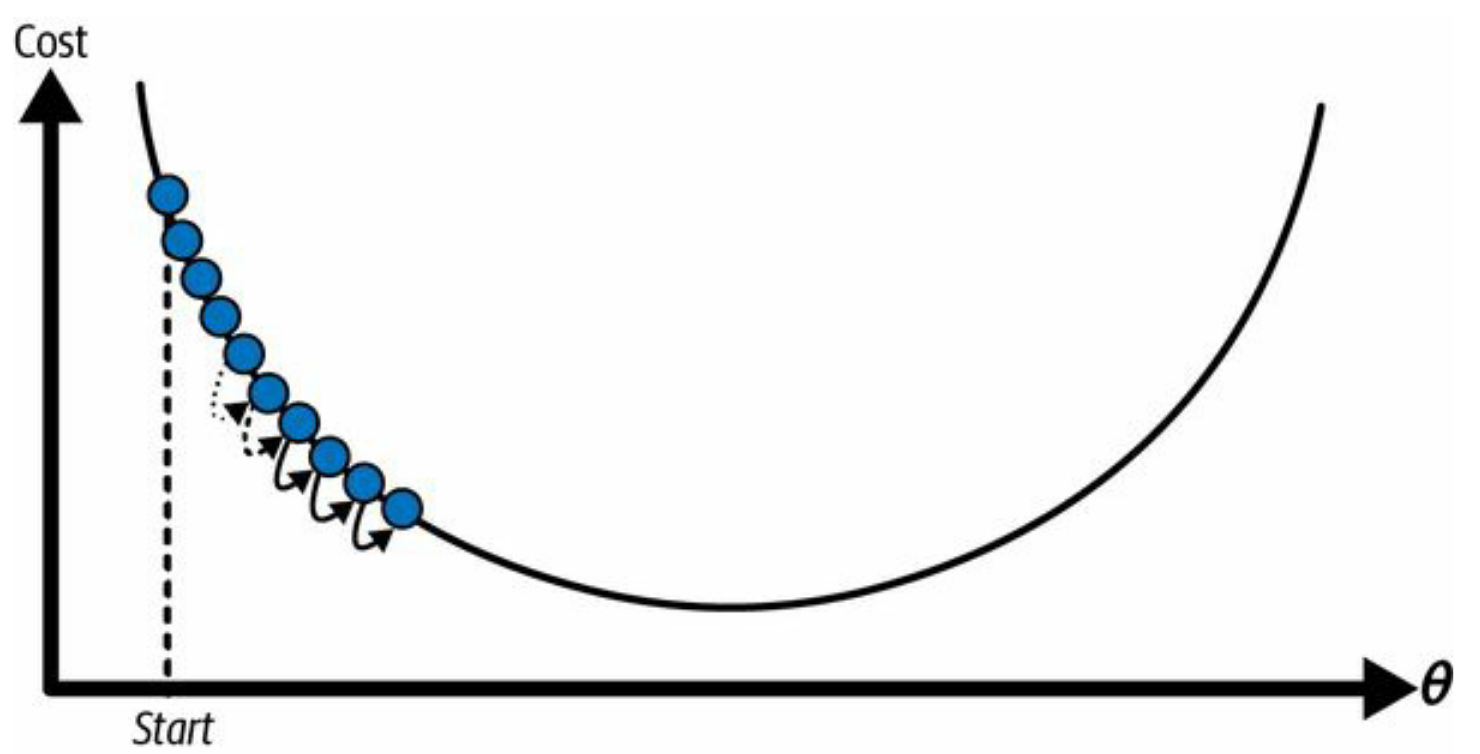
\includegraphics[width=0.5\linewidth, keepaspectratio]{img//chapter4/lr_small.png}\label{fig:lr_small}}
  \hfill
  \subfloat[]{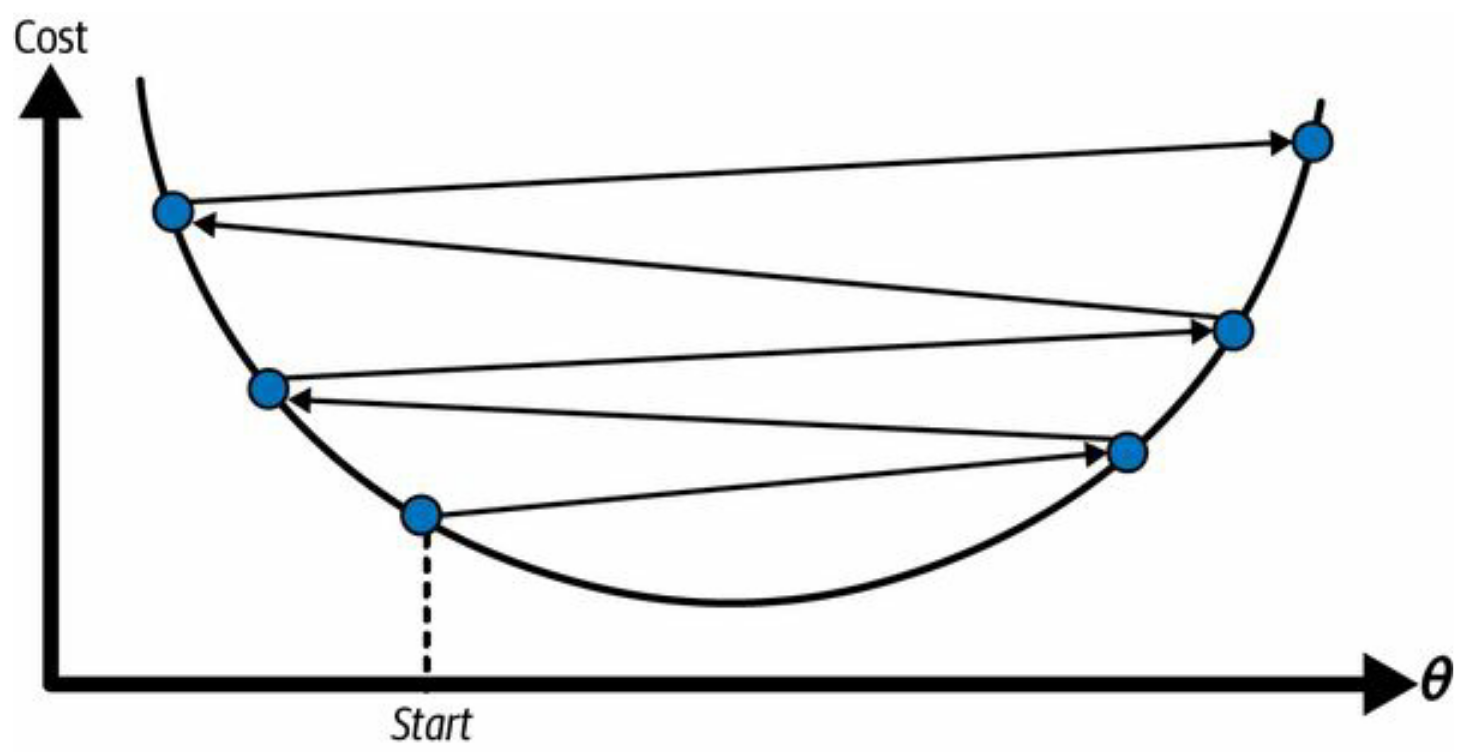
\includegraphics[width=0.5\linewidth, keepaspectratio]{img//chapter4/lr_high.png}\label{fig:lr_high}}
  \caption[Examples of learning rates too small or too high]{Examples of gradient descent for a one-dimensional loss (cost) function with \protect\subref{fig:lr_small} learning rate too small and \protect\subref{fig:lr_high} learning rate too high.\\\small{Credits: \cite{geron_hands-machine_2019}.}}
  \label{fig:lr_small_high}
\end{figure}
\newpage
All gradient-based optimization logic is encapsulated in the \emph{optimizer} object: it determines the direction in which the model parameters should be adjusted and the magnitude of the parameter update (learning rate).

Advanced optimizers, such as Adam \citep{kingma_adam_2017} and AdaDelta \citep{zeiler_adadelta_2012}, go beyond the basic gradient descent by adapting the learning rate during the training process based on the properties of the loss surface (\eg, its curvature). These optimizers can accelerate convergence by dynamically adjusting the step size for each parameter individually, based on the history of gradients. This can be particularly beneficial for navigating complex loss surfaces with varying curvatures.


%%%%%%%%%%%%%%%%%%%%%%%%%%%%%%%%%%%%%%%%%%%%%%%%%%%%%%%
%%%%% SubSubSec: Training loop %%%%%
%%%%%%%%%%%%%%%%%%%%%%%%%%%%%%%%%%%%%%%%%%%%%%%%%%%%%%%
\subsubsection{Training loop}
\label{subsubsec:training_loop}
Having outlined all the essential components within the optimization framework, it is now possible to describe the training process in all its phases, as shown in \cref{fig:backpropagation_algorithm}.
\begin{enumerate}
    \item \textbf{Initialization}: set up the model to be optimized and initialize its parameters to some (random) values.
    \item \textbf{Forward pass}: obtain the model predictions based on the initial parameters and compute the loss to quantify how far the model's outputs are from the actual target/observed values.
    \item \textbf{Backward pass (backpropagation)}: calculate the gradient of the loss function with respect to each parameter in the model. This involves propagating the error backwards from the outputs to the inputs, as described in \cref{subsubsec:reverse_mode}. This process systematically computes the partial derivatives using the chain rule to effectively determine how each parameter should be adjusted to minimize loss.
    \item \textbf{Parameter update (gradient descent)}: for each parameter, update its value by moving it in the direction that minimally decreases the loss
    \be
    \label{eq:4.12}
    \va{\t}_{final} = \va{\t}_{initial} - \eta \va{\nabla}_{\va{\t}_{initial}} f(\va{\t}_{initial}) \,.
    \ee
    \item \textbf{Iteration or convergence}: repeat steps 2 through 4 for a predefined number of iterations (or \emph{epochs}) or until the change in the loss function between iterations falls below a small threshold, indicating convergence.
\end{enumerate}

\begin{figure}
    \centering
    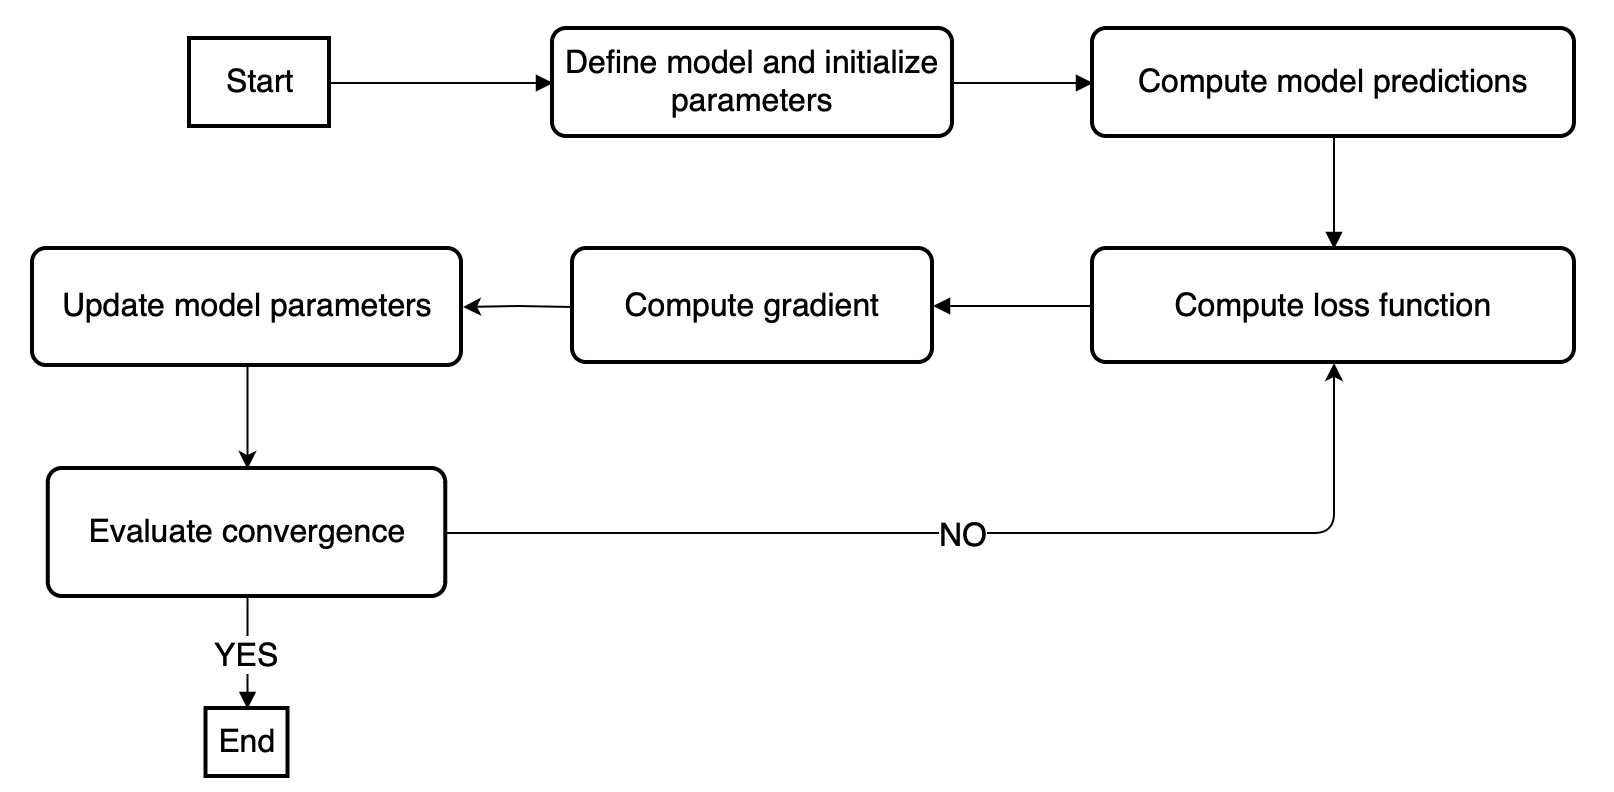
\includegraphics[width=\linewidth, keepaspectratio]{img//chapter4/backpropagation.png}
    \caption[Optimization algorithm diagram]{Optimization algorithm diagram.}
    \label{fig:backpropagation_algorithm}
\end{figure}

The following sections will detail the methods used for the simulation and analysis of the objects presented in \cref{chap:applications}. Beginning with the modeling of light sources and the adopted surface brightness profiles, the discussion will advance to the techniques used for simulating and reconstructing strong gravitational lenses. Finally, methods will be described to assess the accuracy of the model fit to the observed/simulated data.

% *************************************************************
%%%%% SECTION 4.2: LIGHT MODELS %%%%%
%%%%%%%%%%%%%%%%%%%%%%%%%%%%%%%%%%%%%%%%%%%%%%%%%%%%%%%
%%%%% Sec: Light sources modeling  %%%%%
%%%%%%%%%%%%%%%%%%%%%%%%%%%%%%%%%%%%%%%%%%%%%%%%%%%%%%%
\section{Light sources modeling}
\label{sec:light_models}

The prevalent approach to modeling light sources such as galaxies involves using a parametric profile $(R)$, where $R$ represents a measure of distance from the center of the object. These models often presuppose an excessively idealized level of symmetry, yet offer the advantage of being straightforward to define and apply. When building galaxy components, it is generally assumed that the profiles exhibit elliptical symmetry \citep{peng_detailed_2002,peng_detailed_2010}, and therefore $R$ represents the elliptical radius
\be
\label{eq:4.13}
R (\vec{x}^\prime) = \sqrt{{x_1^\prime}^2 + {x_2^\prime / q}^2}
\ee
of a source with an axis ratio $q$. The coordinate system $({x_1^\prime} , {x_2^\prime})$ of the source can be rotated by the \emph{position angle} $\varphi$ with respect to the coordinate system $(x_1 , x_2)$ of the observation. The resulting isophotes\footnote{Curves of constant surface brightness.} of the surface brightness distribution of such an elliptical source are ellipses with semi-major axis $R/q$, semi-minor axis $R$ and orientation $\varphi$ with respect to the $x_1$ axis of observation.


%%%%%%%%%%%%%%%%%%%%%%%%%%%%%%%%%%%%%%%%%%%%%%%%%%%%%%%
%%%%% SubSec: Sérsic profile %%%%%
%%%%%%%%%%%%%%%%%%%%%%%%%%%%%%%%%%%%%%%%%%%%%%%%%%%%%%%
\subsection{Sérsic profile}
\label{subsec:sersic}
The most common model to describe elliptical surface brightness distributions is the \emph{Sérsic law} \citep{sersic_influence_1963,sersic_atlas_1968}, which is given by the exponential
\be
\label{eq:4.14}
I(R) = I_e \exp \bc{- b_n \bs{\bp{\frac{R}{R_{e}}}^{\frac{1}{n}} - 1}} \,,
\ee
where $I_e$ is the surface brightness at the effective radius\footnote{Also called the half-light radius, the radius within which half of the galaxy’s luminosity is contained.} $R_e$ and $n>0$ is called the \emph{Sérsic index}, which characterizes the slope of the profile. The function $b_n$ depends only on the Sérsic index and is defined by
\be
\label{eq:4.15}
\g (2n, b_n) = \frac{1}{2} \G(2n) \,,
\ee
where $\G$, $\g$ are, respectively, the Gamma function and the incomplete Gamma function. It can be shown \citep{ciotti_stellar_1991,ciotti_analytical_1999} that, for a Sérsic index in the range $0.5 \leq n \lesssim 8$, $b_n$ can be approximated by
\be
\label{eq:4.16}
b_n \approx 2n - \frac{1}{3} + \frac{4}{405n} \approx 1.9992n - 0.3271 \,.
\ee
With this, the profile is now fully determined by the seven parameters for position $x_1$, $x_2$, effective radius $R_e$, Sérsic index $n$, intensity at the effective radius $I_e$, axis ratio $q$ and position angle $\varphi$.

The Sérsic profile is a versatile model; by varying $n$ it is possible to obtain many of the classical galaxy profiles as special cases, such as Gaussian profiles ($n = 0.5$), exponential profiles ($n = 1$) and de Vaucouleurs \citep{de_vaucouleurs_recherches_1948} profiles ($n = 4$). 

\begin{figure}
    \centering
    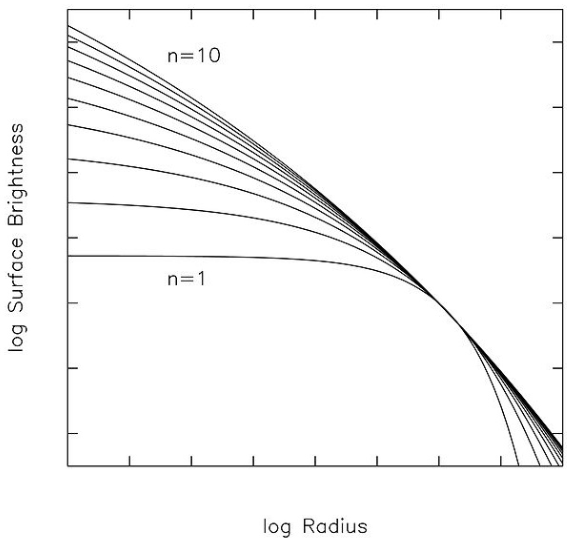
\includegraphics[width=0.65\linewidth, keepaspectratio]{img//chapter4/sersic_n.png}
    \caption[Sérsic profiles for different values of $n$]{Sérsic profiles for different values of $n$. On average, $n \approx 2-10$ for bulges and elliptical galaxies, $n\approx 1$ for disk galaxies and $n \leq 0.5$ for bars and stellar clumps.\\\small{Credits: \cite{burke_assembly_2013}.}}
    \label{fig:sersic_n}
\end{figure}


%%%%%%%%%%%%%%%%%%%%%%%%%%%%%%%%%%%%%%%%%%%%%%%%%%%%%%%
%%%%% SubSec: Core-Sérsic profile %%%%%
%%%%%%%%%%%%%%%%%%%%%%%%%%%%%%%%%%%%%%%%%%%%%%%%%%%%%%%
\subsection{Core-Sérsic profile}
\label{subsec:core_sersic}
An extension of the Sérsic profile has been developed by \cite{graham_new_2003,graham_inner_2004,trujillo_evidence_2004} to better reproduce the observed radial profiles of surface brightness. This model consists of a power law to model the inner radii and a Sérsic function to describe the outer stellar distribution. It is given by
\be
\label{eq:4.17}
I(R) = I^\prime \bs{1 + \bp{\frac{R_b}{R}}^\a}^{\g / \a} \exp{-b_n \bs{\frac{R^\a + R_b^\a}{R_e^\a}}^{1 / (\a n)}} \,,
\ee
where $R_b$ is the break-radius separating the inner power law with logarithmic slope $\g$ from the outer Sérsic profile with slope $n$. The intensity $I_b$ at the break-radius $R_b$ can be evaluated from the expression
\be
\label{eq:4.18}
I^\prime = I_b 2^{- \g / \a} \exp{b_n \bs{\frac{2^{1 / \a} R_b}{R_e}}^{1 / n}} \,.
\ee
The parameter $\a$ controls the sharpness of the transition between the inner (power law) and outer (Sérsic) regimes, with higher values indicating sharper transitions (\cref{fig:core_sersic}).

In this case, the number of parameters becomes larger to include the inner-outer change of regime: the profile is fully determined by ten parameters: for position $x_1$, $x_2$, effective radius $R_e$, Sérsic index $n$, intensity $I_b$ at the break-radius $R_b$, slope of the inner power law $\g$, sharpness of the transition $\a$, axis ratio $q$ and position angle $\varphi$.

\begin{figure}
    \centering
    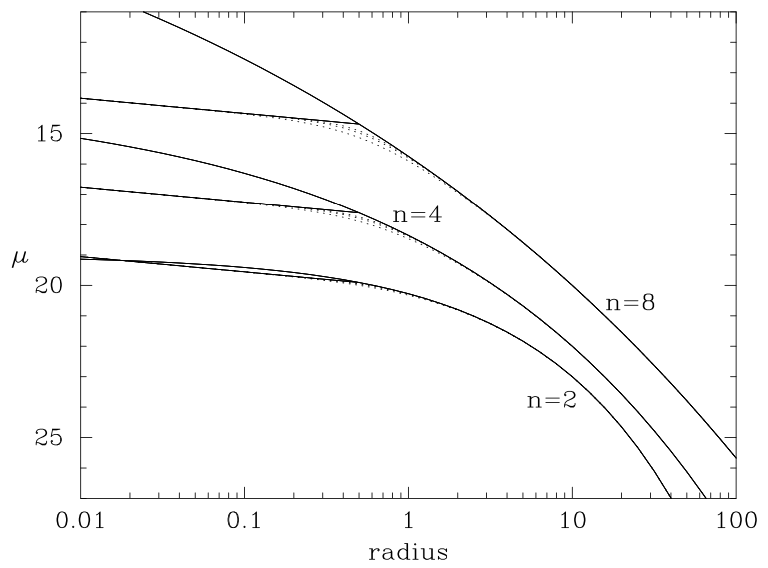
\includegraphics[width=0.7\linewidth, keepaspectratio]{img//chapter4/core_sersic.png}
    \caption[Core-Sérsic profiles for different values of $\a$]{Different core-Sérsic profiles illustrated by the dotted curves for a range of structural parameters. Profiles with values of $\a$ equal to 2, 3, and 4 are shown, the latter giving the sharpest transition. In all models $R_e = \SI{10}{\arcsec}$, $R_b = \SI{0.5}{\arcsec}$, and $\g = 0.2$. For comparison, an inner power law with slope equal to $-0.2$ is shown (diagonal solid lines), as are Sérsic profiles (solid curves) having the same Sérsic shape index $n$.\\\small{Credits: \cite{graham_new_2003}.}}
    \label{fig:core_sersic}
\end{figure}


%%%%%%%%%%%%%%%%%%%%%%%%%%%%%%%%%%%%%%%%%%%%%%%%%%%%%%%
%%%%% SubSec: Sky component  %%%%%
%%%%%%%%%%%%%%%%%%%%%%%%%%%%%%%%%%%%%%%%%%%%%%%%%%%%%%%
\subsection{Sky component}
\label{subsec:sky}
Observations usually include a diffuse distribution of light known as the \emph{sky background}, which must be considered in the reconstruction process. The most basic model for this sky component is a flat surface brightness distribution, characterized by a constant value or a fixed gradient along the $x_1$ and $x_2$ axes of the lens plane. Even if the diffuse background has been removed during a pre-processing step, incorporating a sky component as a free element in the model is advisable. Distinguishing between sky and actual signal is challenging, and any over- or underestimation of the subtracted light can have a considerable impact on the reconstruction outcomes.

%%%%%%%%%%%%%%%%%%%%%%%%%%%%%%%%%%%%%%%%%%%%%%%%%%%%%%%
%%%%% SubSec: Point Spread Function  %%%%%
%%%%%%%%%%%%%%%%%%%%%%%%%%%%%%%%%%%%%%%%%%%%%%%%%%%%%%%
\subsection{Point Spread Function}
\label{subsec:psf}
The Point Spread Function (PSF) is a fundamental concept in optical physics and astronomy that describes how a system blurs or spreads a point light source in an image. The PSF encapsulates the response of an imaging system to a point source or point object, representing the diffraction pattern caused by the optics of the system, including aberrations \citep{bovik_handbook_2005}. Understanding the PSF is crucial for interpreting and processing observational data, as it affects the accuracy with which one can measure the properties of observed objects.

Mathematically, the PSF is often modeled as a convolution kernel that, when applied to an ideal image (the image that would be observed in the absence of any blurring effects), produces the observed image. The process of convolution mathematically
represents spreading the light from point sources over a larger area of the detector, affecting the observed shapes, sizes, and brightness of these objects.

The effect of PSF on an observed image on a plane $(x,y)$ can be described by the convolution of the true image $f(x, y)$ with the Point Spread Function $\mathrm{PSF}(x,y)$, resulting in the observed image $g(x,y)$ \citep{howell_handbook_2006}:
\be
\label{eq:psf}
g(x,y) = (f \ast p)(x,y) = \iint f(x^\prime, y^\prime) \mathrm{PSF}(x - x^\prime, y - y^\prime) \dd{x^\prime} \dd{y^\prime} \,.
\ee


The Point Spread Function (PSF) is usually expressed by means of the Full Width at Half Maximum (FWHM). Their link is rooted in the definition and characterization of the PSF itself. The PSF describes the response of an imaging system to a point source, represented as a distribution or function of intensity across the image plane. The FWHM is a derived characteristic of this distribution, specifically measuring the width of the PSF at half of its maximum intensity.
In the usual case of a Gaussian PSF (\cref{fig:fwhm}):
\be
\label{eq:gauss_psf}
\mathrm{PSF}(x,y) = \mathrm{PSF_0} \exp{- \frac{4 \ln{2}}{\mathrm{FWHM}^2} (x^2 + y^2)} \,,
\ee
where $\mathrm{PSF_0}$ is the peak intensity, the FWHM is directly related to the standard deviation $\s$ of the Gaussian distribution by:
\be
\label{eq:fwhm}
\mathrm{FWHM} = 2 \sqrt{2 \ln{2}} \s \,.
\ee

\begin{figure}
    \centering
    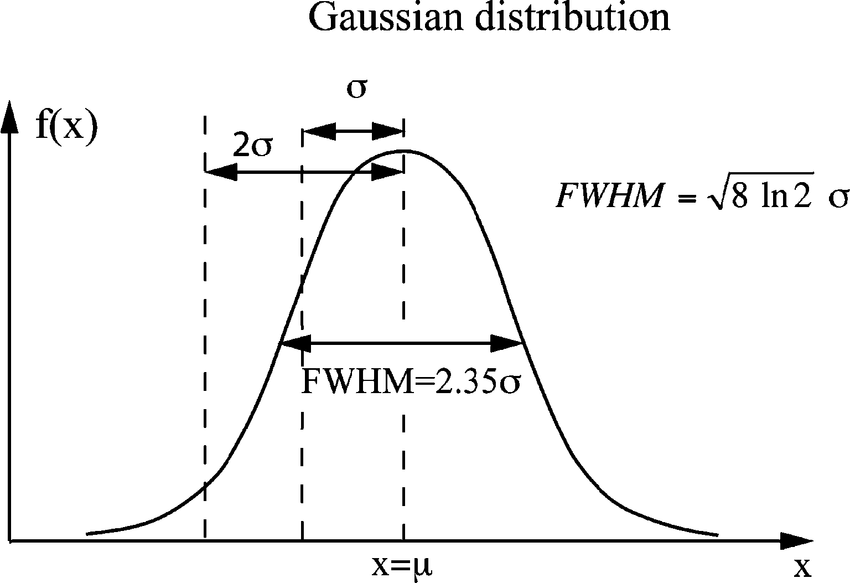
\includegraphics[width=0.6\linewidth]{img//chapter4/fwhm.png}
    \caption[Gaussian PSF and FWHM]{Gaussian or normal PSF and the link with the FWHM.\\\small{Credits: \cite{tavernier_experimental_2010}.}}
    \label{fig:fwhm}
\end{figure}


% *************************************************************
%%%%% SECTION 4.3: LENS INVERSION %%%%%
%%%%%%%%%%%%%%%%%%%%%%%%%%%%%%%%%%%%%%%%%%%%%%%%%%%%%%%
%%%%% Sec: Lens reconstruction  %%%%%
%%%%%%%%%%%%%%%%%%%%%%%%%%%%%%%%%%%%%%%%%%%%%%%%%%%%%%%
\section{Lens reconstruction}
\label{sec:lens_reconstruction}

One of the primary applications of gravitational lensing is reconstructing the lens mass distribution. The modeling of gravitational lenses begins with a collection of observables (\cref{fig:observables}), such as the relative positions and fluxes of images, time delays between images, and other properties of the lens. This modeling can be approached in one of two different but related ways: as a \emph{forward} problem of creating a model of the lens system (lenses and sources) that approximates the observed image the best, or as the \emph{inverse} problem of finding a lens model that deconstructs the observation into a self-consistent and physically viable image of the source. Many successful applications have been published for both the forward \citep{bandara_witnessing_2013,bolton_sloan_2008,newton_sloan_2011,peng_probing_2006} and the inverse method \citep{dye_decomposition_2005,kochanek_lensclean_1992,nightingale_adaptive_2015,suyu_bayesian_2006,vegetti_bayesian_2009,wallington_lensmem_1996,warren_semilinear_2003}.

\begin{figure}
    \centering
    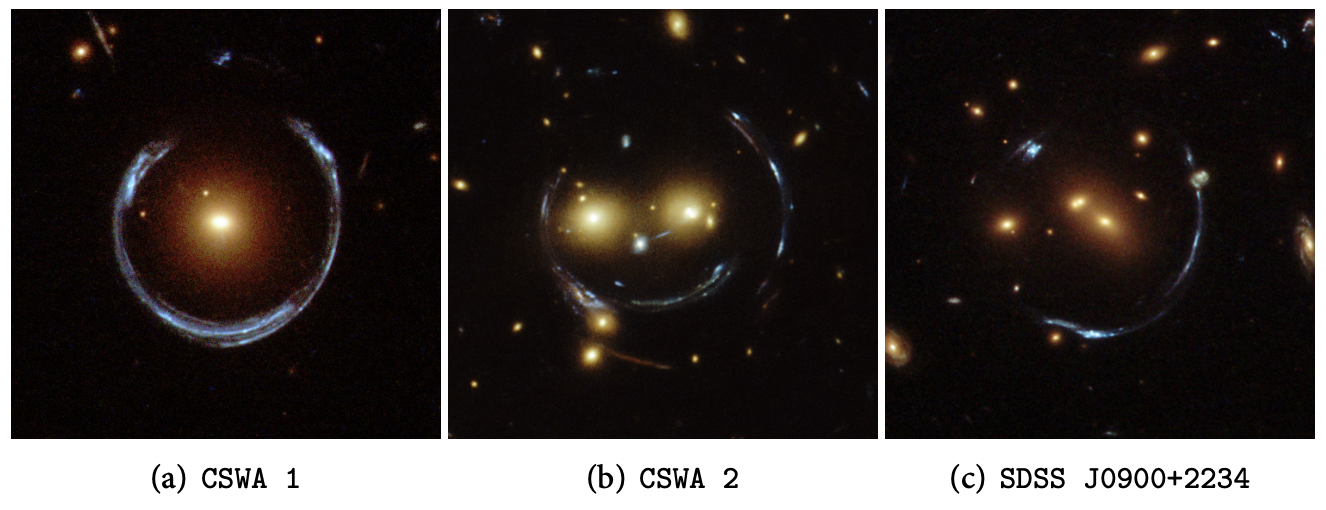
\includegraphics[width=\linewidth, keepaspectratio]{img//chapter4/observables.png}
    \caption[Strong gravitational lensing observations]{Examples of observations of strong gravitational lensing. The large arcs contain information to constrain the gravitational lenses producing these images. \small{Credits: ESA/Hubble $\&$ Nasa}.}
    \label{fig:observables}
\end{figure}

Three types of constraints can be used for this purpose:
\begin{enumerate}
    \item the locations of the multiple images produced by a lensed source help to map out the deflection field of the lens, which corresponds to the first derivatives of the lensing potential \citep{cardone_gravitational_2001}. Obtaining these constraints is relatively straightforward assuming the availability of high-resolution imaging data. This work will mainly focus on this type of constraint.
    \item the magnifications (fluxes) and shapes of the multiple images and gravitational arcs explore the higher-order derivatives (mainly the second) of the lensing potential \citep{gilman_probing_2019}. Therefore, these constraints are particularly sensitive to the smaller-scale mass components of the lens;
    \item the relative time delays between multiple images serve as probes of the lensing potential, as shown in \cref{subsec:time_delay_images}. However, time delays can only be measured in a limited number of lenses (only a few tens) because they require the lensed sources to be intrinsically variable, such as quasars or supernovae \citep{refsdal_possibility_1964}. These types of source are rare. Additionally, measuring time delays is challenging; it demands dedicated telescope time for the continuous observation of these sources over extended periods, along with precise photometry.
\end{enumerate}

The method of translating observed strong lensing constraints into distributions of matter is referred to as lens \emph{inversion} or \emph{reconstruction}.

Such reconstruction is often tackled using two main categories of inversion algorithms \emph{parametric} and \emph{non-parametric} algorithms, based on whether the calculation is ``model-based'' (parametric) or ``model-free'' (non-parametric) at the start of the process \citep{coe_lensperfect_2008}. This work is focused on the first type of approach, applying parametric optimization to retrieve the mass distribution of the lens.

Each approach has its own particular set of strengths and weaknesses, which are summarized here.
\begin{enumerate}

    \item Parametric models employ a clear physical parameterization from the beginning, defining the mass distribution based on a set of specific parameters. Parametric simulation models are generally used to solve the forward problem, taking a source and lensing mass and then predicting the resulting image. Also known as simply-parameterized models, they assume a physical model that fits the data with relatively few defined parameters \citep{jullo_bayesian_2007}. In parametric models, the data is fitted to a physical object (\eg Point-Mass, Singular Isothermal Sphere, Singular Isothermal Ellipsoid, De Vaucouleurs model, etc.) and a model of the lensing mass made using that physical object to predict the effect on the light from the source, often with the assumption that mass follows light. The exploration of these models parameter space aims to identify the optimal combination that accurately replicates the observed positions, shapes, magnitudes, and relative time delays of the multiple images and arcs;

    \item non-parametric methods, which do not start with a predefined physical model but instead use a ``grid-based'' approach, among others, to model the mass distribution. The lens is divided into a mesh, which can be either structured or unstructured, and the lensing observables are projected onto this mesh. Subsequently, this mesh is converted into a pixelized mass distribution using the relationships between the observables and the surface density of the lens. This technique has been extensively applied on a variety of scales, from galaxies to clusters, and has been implemented in numerous ways \citep{birrer_gravitational_2015,blandford_modeling_2000,coles_gravitational_2014,diego_non-parametric_2005,diego_combined_2007,koopmans_gravitational_2005,liesenborgs_genetic_2006,merten_mesh-free_2016,saha_portable_2004,sebesta_testing_2016,suyu_anatomy_2006,suyu_dissecting_2009}.
\end{enumerate}


%%%%%%%%%%%%%%%%%%%%%%%%%%%%%%%%%%%%%%%%%%%%%%%%%%%%%%%
%%%%% SubSec: Parametric reconstruction %%%%%
%%%%%%%%%%%%%%%%%%%%%%%%%%%%%%%%%%%%%%%%%%%%%%%%%%%%%%%
\subsection{Parametric reconstruction}
\label{subsec:parametric_reconstruction}
Strong lensing parametric reconstruction, also known as inversion, involves the use of predefined models to describe both the mass distribution of the lensing object and the light distribution of the background source. The aim is to adjust the parameters of these models to best fit the observed lensing phenomena, such as arcs, rings, and multiple images of a background source. The process is detailed and involves several key steps and algorithms:
\begin{enumerate}
    \item \textbf{model selection} for both the mass distribution and the light distribution;
    \item \textbf{parameter initialization} for the parameters of the mass and light distribution models are made based on observational data or theoretical considerations;
    \item \textbf{ray-tracing simulation} using the initial models: a ray-tracing algorithm computes the deflection angles at each point in the lens plane, which are used to trace the light rays back to the source plane. This step predicts the appearance of the lensed images based on the current model parameters;
    \item \textbf{optimization} via an objective (loss) function that quantifies the difference between the observed and predicted lensed images, as described in \cref{sec:diff_prog}. This function often includes terms for the positions, shapes, and flux ratios of the observed and model-predicted images. Methods such as gradient descent \citep{ruder_overview_2016,canu_introduction_2016}, Markov Chain Monte Carlo (MCMC) \citep{geyer_practical_1992,speagle_conceptual_2019}, or Nested-Sampling \citep{skilling_nested_2004,buchner_nested_2023} are used to adjust model parameters to minimize the objective function. This iterative process refines the model to better fit the observations;
    \item \textbf{model comparison and selection} if multiple models are being tested, and statistical criteria such as the Akaike Information Criterion (AIC) \citep{cavanaugh_akaike_2019} or Bayesian Information Criterion (BIC) \citep{liddle_information_2007,chen_extended_2008} are used to compare their fit to the data, helping to select the best model;
    \item \textbf{uncertainty quantification} for the model parameters, often through bootstrapping or by analyzing the posterior probability distributions in methods like MCMC, providing insights into the confidence levels of the mass and light distribution parameters.
\end{enumerate}

As already stated, parametric reconstruction is highly dependent on the chosen models and their ability to accurately represent the complex mass distributions of astronomical objects. Its strength lies in its relatively straightforward interpretation and the physical significance of the model parameters, but it also faces limitations in flexibility compared to non-parametric methods.

There are several ways to implement parametric lens reconstruction and, as will be shown in \cref{chap:applications}, one of the most common approaches is to use the observed positions of multiple images (\cref{fig:multiple_images_param}).
The optimization can then be performed in mainly two ways: with the so-called \emph{lens} or \emph{image plane optimization} or with the \emph{source plane optimization} technique.

\begin{figure}
    \centering
    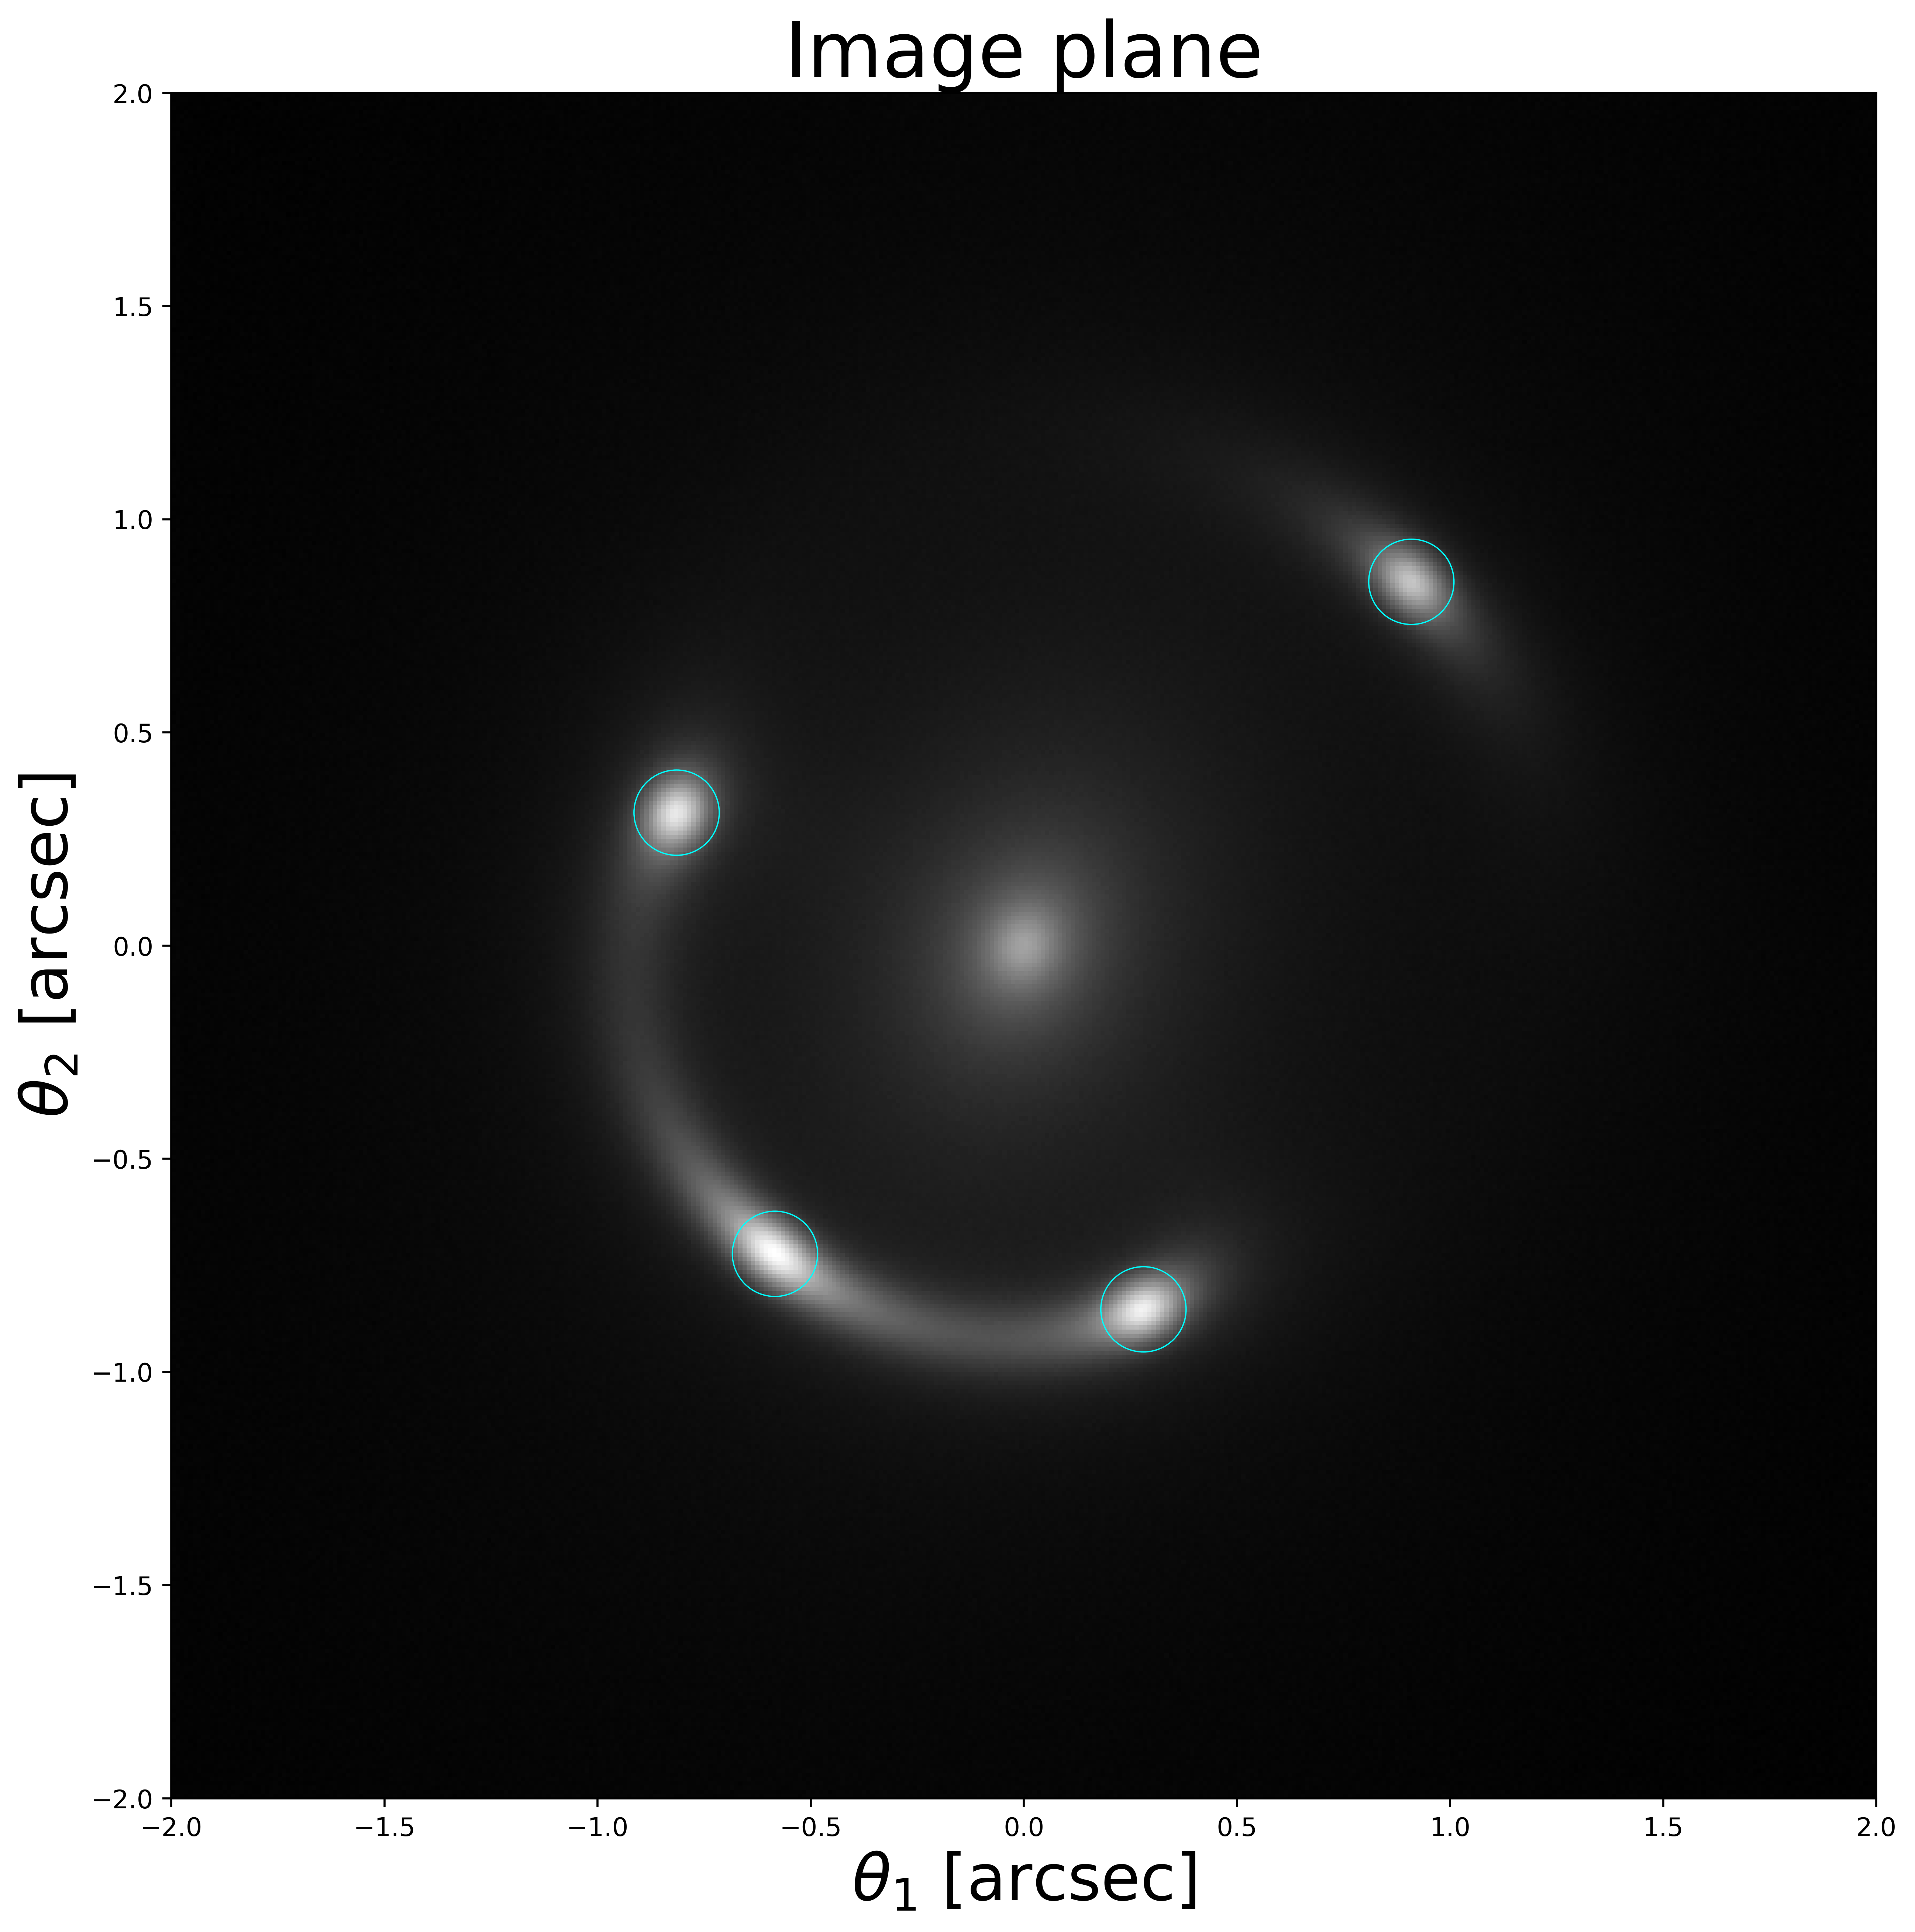
\includegraphics[width=0.6\linewidth, keepaspectratio]{img//chapter4/multiple_images_param.png}
    \caption[Simulated image of a strong lensing event with multiple images]{Simulated image of a strong lensing event with multiple images, indentified by the azure circles. The image is $\SI{4}{\arcsecond} \times \SI{4}{\arcsecond}$, with a pixel scale of $\SI{0.03}{\arcsecond}$.}
    \label{fig:multiple_images_param}
\end{figure}

%%%%%%%%%%%%%%%%%%%%%%%%%%%%%%%%%%%%%%%%%%%%%%%%%%%%%%%
%%%%% SubSubSec: Lens plane and source plane optimization %%%%%
%%%%%%%%%%%%%%%%%%%%%%%%%%%%%%%%%%%%%%%%%%%%%%%%%%%%%%%
\subsubsection{Lens plane and source plane optimization}
\label{subsubsec:lens_plane_source_plane_optimization}
In the context of lens inversion, the positions of multiple images $\va{\t}_i$ are the main observable feature that can be used to constrain the lens parameters. It is assumed that the lens is described by a surface density model (\eg SIS, SIE, etc.) depending on a set of $n$ parameters $\vec{p} = [p_1, \ldots, p_n]$, starting at some initial values (random or constrained by other observables) and that the redshifts of the source and lens are known.

\begin{itemize}
    \item \textbf{Lens plane optimization}

    Given a set of lens parameters, it is possible to calculate the lens deflection angle at the observed positions of the images $\va{\a} (\va{\t}_i | \vec{p})$ and, using the lens equation, map these positions on the source plane:
    \be
    \label{eq:4.19}
    \va{\b}_i (\vec{p}) = \va{\t}_i - \va{\a} ( \va{\t}_i | \vec{p}) \,.
    \ee

    The resulting points $\va{\b}_i (\vec{p})$ will be spread over a certain region in the source plane since the model parameters are not correct. The predicted source position can be estimated by taking the mean position of these points:
    \be
    \label{eq:4.20}
    \va{\b} (\vec{p}) = \frac{1}{N_{ima}} \sum\limits_{i=1}^{N_{ima}} \va{\b}_i (\vec{p}) \,,
    \ee
    where $N_{ima}$ is the observed number of multiple images.

    Subsequently, by solving the lens equation, the predicted source position can be mapped back to the lens plane, obtaining a set of predicted image positions
    \be
    \label{eq:4.21}
    \va{\b} (\vec{p}) \rightarrow \{\va{\t}_i (\vec{p}) ; i = 1, \ldots, N_{ima, \vec{p}}\} \,,
    \ee
    where the number of predicted images, $N_{ima, \vec{p}}$, can clearly be different from $N_{ima}$.

    At this point a cost function can be defined to compare the predicted and observed positions of the images
    \be
    \label{eq:4.22}
    \chi^2 (\vec{p}) = \sum\limits_{i=1}^{N_{ima}} \frac{[\va{\t}_i - \va{\t}_i (\vec{p})]^2}{\s_i^2} \,,
    \ee
    where $\va{\t}_i (\vec{p})$ is the position of the predicted image closest to the image at $\va{\t}_i$ and $\s_i$ is the error on the position of the $i$-th image.

    To identify the optimal lens model, one can adjust the parameters $\vec{p}$ to minimize the loss function, or equivalently, to maximize the likelihood of the observed image positions given the parameters $\vec{p}$
    \be
    \label{eq:4.23}
    \mathscr{L} (\vec{p}) = \frac{1}{\prod\limits_{i=1}^{N_{ima}} \s_i \sqrt{2 \pi}} \exp \left[ - \frac{\chi^2 (\vec{p})}{2} \right] \,.
    \ee

    When dealing with multiple families of multiple images, the same approach can be utilized. However, the likelihood function must be adjusted to become the product of the likelihoods corresponding to each image family
    \be
    \label{eq:4.24}
    \mathscr{L} (\vec{p}) = \prod\limits_{j=1}^{N_{fam}} \frac{1}{\prod\limits_{i=1}^{N_{ima}} \s_{ji} \sqrt{2 \pi}} \exp \left[ - \frac{\chi_j^2 (\vec{p})}{2} \right] \,,
    \ee
    with $\chi_j^2$ as defined in \cref{eq:4.22}, but referring to the $j$-th family of multiple images and $\s_{ji}$ is the error on the position of the $i$-th image of the $j$-th family.

    Maximizing the aforementioned likelihood is equivalent to minimizing the total chi-squared value $\chi_{tot}^2$, which is defined by
    \be
    \label{eq:4.25}
    \chi_{tot}^2 (\vec{p}) = \sum\limits_{j=1}^{N_{fam}} \chi_j^2 (\vec{p}) \,.
    \ee
    \clearpage
    \item \textbf{Source plane optimization}

    An alternative to optimizing in the lens plane is to perform optimization in the source plane. In an ideal scenario, if the model parameters precisely match the lens parameters, multiple images would map to a single position on the source plane. Consequently, a cost function can this time be defined on the source plane to facilitate this optimization process
    \be
    \label{eq:4.26}
    \chi_s^2 (\vec{p}) = \sum\limits_{i=1}^{N_{ima}} \frac{[\va{\b}_i (\vec{p}) - \va{\b} (\vec{p})]^2}{ \s_i^2} \mu_i (\vec{p})^2 \,,
    \ee
    where $\mu_i (\vec{p})$ is the model estimated magnification at the $i$-th image position.
\end{itemize}


The primary benefit of source plane optimization is the elimination of the most complex step in the previously described lens plane optimization procedure. This step, which involves solving the lens equation, can be computationally intensive and is typically addressed by numerical methods. When leveraging multiple families of images as constraints, optimization on the lens plane becomes considerably more time consuming compared to source plane optimization. Furthermore, this approach does not require a one-to-one match between the observed and predicted images by the model when calculating the chi-squared $\chi^2$. However, a potential downside is that the error for each predicted source position $\b_i (\vec{p})$ must be estimated using the model-predicted magnification $\mu_i (\vec{p}) = \mu (\va{\t}_i | \vec{p})$ at the image positions. Additionally, optimization on the source plane may produce biased solutions, often favoring models with flatter density profiles and higher ellipticity \citep{kneib_cluster_2011}.



% *************************************************************
%%%%% CHAPTER 5: APPLICATIONS %%%%%
\cleardoublepage
\chapter{Applications}
\label{chap:applications}

In the following sections, we discuss specific lensing applications on three different scales.
Our discussion initiates with a detailed examination of microlensing events, phenomena where the gravitational field of a relatively small object, such as a star or planet, magnifies the light of a background star. This section will focus on the technique of light-curve fitting, a method that analyzes the temporal change in brightness of the lensed star to extract critical information about the lensing object. Microlensing offers a unique method for detecting elusive objects, including exoplanets \citep{sumi_unbound_2011,gaudi_microlensing_2012} and dark compact objects, providing insights into the mass, motion, and distribution of such entities within the Milky Way \citep{alcock_possible_1993,udalski_optical_1993}.

Transitioning from the stellar to the galactic scale, we next explore the realm of galaxy-scale lensing \citep{treu_strong_2010} by optimizing a parametric strong lensing model. This segment emphasizes the development and optimization of parametric models for strong lensing, where entire galaxies act as lenses, distorting and magnifying the light of more distant galaxies into arcs and rings. Through the optimization of these models, we aim to reconstruct the mass distribution of lensing galaxies \citep{auger_sloan_2010}, including the elusive dark matter component \citep{vegetti_detection_2010}. This approach not only sheds light on the structure and composition of galaxies, but also contributes to our understanding of the evolution of the large-scale structure of the Universe.

Finally, we will address weak lensing by fitting surface brightness profiles and measuring ellipticities.

% *************************************************************
%%%%% SECTION 5.1:  Fit of microlensing light curve %%%%%
\section{Microlensing light-curve fit}
\label{sec:fit_micro}

The standard microlensing light-curve, also known as the Paczynski light-curve, \citep{paczynski_gravitational_1986}, as introduced in \cref{sec:microlenses}, is defined by three parameters: the impact parameter $y_0$, the maximum magnification time $t_0$, and the Einstein radius crossing time $t_E$, which represents the time scale of the microlensing event. The latter implicitly depends on other relevant quantities of the lensing system, the lens mass $M$, the relative velocity between lens and source $v_{rel}$ and the distances between lens and source from the observer $D_L$ and $D_S$. The combination of these parameters defines the amplification to which a source with intrinsic flux $f_S$ is subjected.

The first step consists of simulating a microlensing event to obtain synthetic observational data, to which noise is then added in such a way as to mimic observational errors. We start by considering a lens with mass $M = \SI{0.3}{\msun}$ placed at a distance $D_L = \SI{4.0}{\kilo\parsec}$. We then define a source behind the lens, at a distance $D_S = \SI{8.0}{\kilo\parsec}$, characterized by an intrinsic flux of $f_S = 7.0$ (in arbitrary units), which moves with relative velocity $v_{rel} = \SI{200.0}{\kilo\meter\per\second}$ with respect to the lens. Assuming that one could monitor the source for a long period (one year in this case), a microlensing event happens when the source moves across the Einstein radius of the lens, causing a peak in the magnification. In this simulation, this occurs at $t_0 = \SI{183.0}{\day}$. After setting up the model parameters, shown in \cref{tab:parameters_micro_0}, the simulated light curve can be computed and the result is shown in \cref{fig:initial_model_micro} (black dots). The errors in the photometric measurement are assumed to be $10\%$ of the baseline flux.
Subsequently, the model was initialized with random parameters. Predictions of the model, given the set of initial parameters, are shown in \cref{fig:initial_model_micro} (red line), along with the standardized residuals, which are expressed in units of standard deviation from the mean.

\begin{figure}
  \begin{minipage}{\linewidth}
    \centering
    \subfloat[]{\includegraphics[width=\linewidth, keepaspectratio]{img/chapter5/microlensing/lc_initialmodel.png}\label{fig:lc_initialmodel}}
  \end{minipage}
  \begin{minipage}{\linewidth}
    \centering
    \subfloat[]{\includegraphics[width=\linewidth, keepaspectratio]{img/chapter5/microlensing/residuals_init.png}\label{fig:residuals_init}}
  \end{minipage}
  \caption[Microlensing initial predictions and residuals]{\protect\subref{fig:lc_initialmodel} Initial predictions of the model and \protect\subref{fig:residuals_init} residuals expressed in units of standard deviation from their mean.}
  \label{fig:initial_model_micro}
\end{figure}

\clearpage

\begin{table}[t]
\setlength{\extrarowheight}{2pt}
\setlength{\tabcolsep}{1pt}
\centering
\caption{Summary of the parameters before and after fitting the model with the set of degenerate parameters.}
\label{tab:parameters_micro_0}
%\resizebox{0.2\linewidth}{!}{
\begin{tabular}{@{}c@{\hskip 10pt}c@{}@{\hskip 10pt}c@{}@{\hskip 10pt}c@{}@{\hskip 10pt}c@{}}
\toprule
Parameter         & True value                          & Initial value                        & Best-fit value                           & Best-fit value                                                              \\
                  &                                     &                                      & (degeneracy)                             & (MCMC)                                                                      \\ \midrule
$f_S$             & \SI{7.0}{}                          & \SI{2.0}{}                           & \SI{6.993}{}                            & \SI[separate-uncertainty=true]{7.017 \pm 0.040}{}                         \\
$M$               & \SI{0.3}{\msun}                     & \SI{0.8}{\msun}                      & \SI{0.556}{\msun}                       & \SI[separate-uncertainty=true]{0.620 \pm 0.466}{\msun}                    \\
$y_0$             & \SI{0.1}{}                          & \SI{0.6}{}                           & \SI{0.100}{}                            & \SI[separate-uncertainty=true]{0.101 \pm 0.001}{}                         \\
$v_{rel}$         & \SI{200.0}{\kilo\meter\per\second}  & \SI{180.0}{\kilo\meter\per\second}   & \SI{182.881}{\kilo\meter\per\second}    & \SI[separate-uncertainty=true]{231.722 \pm 49.037}{\kilo\meter\per\second}\\
$t_0$             & \SI{183.0}{\day}                    & \SI{114.0}{\day}                     & \SI{183.002}{\day}                      & \SI[separate-uncertainty=true]{183.018 \pm 0.023}{\day}                   \\
$D_L$             & \SI{4.0}{\kilo\parsec}              & \SI{2.0}{\kilo\parsec}               & \SI{1.548}{\kilo\parsec}                & \SI[separate-uncertainty=true]{3.166 \pm 1.698}{\kilo\parsec}             \\
$D_S$             & \SI{8.0}{\kilo\parsec}              & \SI{7.0}{\kilo\parsec}               & \SI{3.786}{\kilo\parsec}                & \SI[separate-uncertainty=true]{8.658 \pm 3.457}{\kilo\parsec}             \\ \bottomrule
\end{tabular}
%}
\end{table}

After initializing the model, the cost function was defined to quantify the discrepancy between the model and the observed data. In this case, a reduced chi-square $\chi_\n^2$ was specified as the metric of choice. It is defined as
\be
\label{eq:5.01}
\chi_\nu^2 = \frac{\chi^2}{\nu} = \frac{1}{\nu} \sum\limits_{i} \bs{\frac{(O_{i} - E_{i})^2}{\s_i^2}} \,,
\ee
where $O_i$ and $E_i$ are the $i$-th observed and expected values respectively, while $\s_i$ is the data uncertainty on the $i$-th observed value. The term $\nu$ represents the degrees of freedom, calculated as the number of observations minus the number of fitted parameters. A value of $\chi_\n^2$ close to 1 suggests that the model fits the data well, with deviations between the observed and expected values largely attributable to random noise. A value significantly greater than 1 indicates that the model does not fit the data well, possibly due to systematic errors, an incorrect model, or an underestimation of the variability in the data. On the contrary, a value significantly less than 1 may suggest that the model fits the data too well, potentially due to overfitting or overestimation of the variability in the data.

At this stage, Adam \citep{kingma_adam_2017} is set as the optimizer to perform a gradient descent optimization on the cost function of choice and minimize its value by updating the model parameters at each iteration. Training starts with a loss value of $\chi_\n^2 = 192.939$ and, after 1000 iterations, the algorithm stops after reaching a $\chi_\n^2 = 1.028$.

As can be seen \cref{tab:parameters_micro_0}, even though the input parameters $f_S$, $y_0$ and $t_0$ are accurately estimated, almost matching their true values precisely, the other parameters show considerable deviation from their actual values. This discrepancy was expected and, as introduced in \cref{sec:microlenses}, is due to the high microlensing degeneracy, as these parameters collectively influence the determination of the Einstein crossing time $t_E$. In fact, it is the Einstein crossing time alone that shapes the light curve's profile.

This degeneracy can also be seen after performing a Bayesian sampling of the posterior probability distribution of the parameters using the Monte Carlo Markov Chain (MCMC) sampler implemented in the \texttt{Pyro}\footnote{\url{https://pyro.ai/}} framework \citep{bingham_pyro_2018}, which is a probabilistic programming language built on top of \texttt{PyTorch}, designed to create and run complex probabilistic models. The resulting posterior probability distributions of the parameters are shown in \cref{fig:corner_micro_bad}. In the literature, numerous methods have been known to attempt to break this degeneracy \citep{lee_microlensing_2017}. In this case, the choice was made to redefine the model so that it directly depends on $t_E$, a quantity that, as mentioned, implicitly contains all the degenerate parameters within it.

\begin{figure}
    \centering
    \includegraphics[width=\linewidth, keepaspectratio]{img//chapter5//microlensing/corner_bad.png}
    \caption[Microlensing corner plot showing degeneracy]{Corner plot showing the posterior probability distributions of the parameters used to fit the light-curve in \cref{fig:lc_initialmodel}. The projections of the probability density on planes defined by each couple of parameters, as well as one-dimensional marginalized distributions are shown. The degeneracy among the parameters $M$, $v_{rel}$, $D_L$ and $D_S$ is clearly visible.}
    \label{fig:corner_micro_bad}
\end{figure}

The fitting procedure for the simulated observations was therefore repeated, defining a model with the same initial parameters but fitting only the parameters $f_S$, $t_0$, $y_0$ and $t_E$. In this case, the initial reduced chi-square value is $\chi_\n^2 = 193.270$, and after training the model for the same number of epochs as before, it drops to a value of $\chi_\n^2 = 1.009$. The best-fit parameters are indicated in \cref{tab:parameters_micro_1}, while \cref{fig:final_model_micro,fig:micro_loss} show, respectively, the best-fit model with its standardized residuals, and the trend of the cost function as a function of the number of iterations.

\begin{table}
\setlength{\extrarowheight}{2pt}
\setlength{\tabcolsep}{1pt}
\centering
\caption{Summary of the parameters before and after fitting the model a second time to avoid degeneracy.}
\label{tab:parameters_micro_1}
%\resizebox{0.2\linewidth}{!}{
\begin{tabular}{@{}c@{\hskip 20pt}c@{}@{\hskip 20pt}c@{}@{\hskip 20pt}c@{}@{\hskip 20pt}c@{}}
\toprule
Parameter           & True value                            & Initial value                        & Best-fit value         & Best-fit value                                            \\
                    &                                       &                                      & (training)             & (MCMC)                                                    \\\midrule
$f_S$               & \SI{7.0}{}                            & \SI{2.0}{}                           & \SI{7.065}{}          & \SI[separate-uncertainty=true]{7.052 \pm 0.041}{}       \\
$M$\anote           & \SI{0.3}{\msun}                       & \SI{0.8}{\msun}                      &                        &                                                           \\
$y_0$               & \SI{0.1}{}                            & \SI{0.6}{}                           & \SI{0.103}{}          & \SI[separate-uncertainty=true]{0.100 \pm 0.001}{}       \\
$v_{rel}$\anote     & \SI{200.0}{\kilo\meter\per\second}    & \SI{180.0}{\kilo\meter\per\second}   &                        &                                                           \\
$t_0$               & \SI{183.0}{\day}                      & \SI{114.0}{\day}                     & \SI{182.989}{\day}    & \SI[separate-uncertainty=true]{183.010 \pm 0.022}{\day} \\
$D_L$\anote         & \SI{4.0}{\kilo\parsec}                & \SI{2.0}{\kilo\parsec}               &                        &                                                           \\
$D_S$\anote         & \SI{8.0}{\kilo\parsec}                & \SI{7.0}{\kilo\parsec}               &                        &                                                           \\
$t_E$               & \SI{19.1369}{\day}                    & \SI{29.3461}{\day}                   & \SI{19.025}{\day}   & \SI[separate-uncertainty=true]{19.054 \pm 0.207}{\day}  \\ \bottomrule
\end{tabular}
%}
\smallskip
\parbox[]{0.9\textwidth}{\footnotesize
  \textit{*:}
  Parameters not fitted to avoid degeneracy.
}
\end{table}

\begin{figure}
  \begin{minipage}{\linewidth}
    \centering
    \subfloat[]{\includegraphics[width=\linewidth, keepaspectratio]{img/chapter5/microlensing/best_fit.png}\label{fig:lc_finalmodel}}
  \end{minipage}
  \begin{minipage}{\linewidth}
    \centering
    \subfloat[]{\includegraphics[width=\linewidth, keepaspectratio]{img/chapter5/microlensing/residuals_best.png}\label{fig:residuals_final}}
  \end{minipage}
  \caption[Microlensing initial predictions and residuals]{\protect\subref{fig:lc_finalmodel} Predictions of the best-fit model and \protect\subref{fig:residuals_final} residuals expressed in units of standard deviation from their mean.}
  \label{fig:final_model_micro}
\end{figure}

\begin{figure}
    \centering
    \includegraphics[width=\linewidth, keepaspectratio]{img//chapter5//microlensing/corner_good.png}
    \caption[Microlensing corner plot non degenerate parameters]{As \cref{fig:corner_micro_bad} but for a model whose free parameters are $f_S$, $t_0$, $y_0$, $t_E$.}
    \label{fig:corner_micro_good}
\end{figure}

\begin{figure}[H]
    \centering
    \includegraphics[width=\linewidth, keepaspectratio]{img//chapter5//microlensing/loss.png}
    \caption[Microlensing loss value as a function of epochs]{Loss value as a function of epochs.}
    \label{fig:micro_loss}
\end{figure}

% *************************************************************
%%%%% SECTION 5.2:  Fit of microlensing light curve %%%%%
\section{Strong lens parametric reconstruction}
\label{sec:strong_lens}

This section of the thesis delves into the intricacies of parametric strong lensing, focusing on the Singular Isothermal Ellipsoid (SIE) model, a widely adopted representation for the mass distribution of lensing galaxies. The SIE model provides a robust framework for simulating gravitational lenses, offering a simplified, yet effective, portrayal of their mass profiles.

Taking advantage of the positions of multiple images generated by the lensing effect, one can derive the parameters of the lensing system that produced them. The objective is to optimize the lens parameters, which dictate the lensing behavior and, consequently, the appearance and positions of the lensed images.

This optimization is pursued through two distinct methodologies, as discussed in \cref{sec:lens_reconstruction}. Starting in both techniques from the positions of the multiple images, the first method focuses on optimizing the lens parameters within the source plane, by mapping the positions of the images back in the source plane and minimizing the distance between the theoretical and inferred position of the source.

The second method shifts the focus to the lens plane by directly minimizing the distances between each observed and predicted image to optimize the lens parameters.

\subsection{Lens modelling}
\label{subsec:lens_modelling}
The first step, as always, is to produce a simulation of the lensing system and the main observables of this topic, the multiple images of the background source.

The process begins by defining the observational parameters: a grid of $100 \times 100 \,\SI{}{\pixel}$ is established, with a resolution of $\SI{0.03}{\arcsecond\per\pixel}$. A background noise per pixel of $rms = 0.5$ mimics real observational noise. Additionally, the final image is also convolved with a Gaussian PSF with FWHM of $\SI{0.1}{\arcsecond}$. Subsequently, the definition of the lens and source hyperparameters follows. Regarding the mass distribution of the lens, an SIE model is assumed in the center of the grid, at position $(0,0)$, characterized by a velocity dispersion of $\SI{200.0}{\kilo\meter\per\second}$, axial ratio of $0.3$ and position angle of $\SI{45}{\deg}$. Concerning the surface brightness distribution, a Sérsic profile is assumed for both objects: for the lens, an effective radius of $\SI{5.0}{\arcsecond}$ and a Sérsic index $n = 3.5$, while for the source these parameters are set to $\SI{0.3}{\arcsecond}$ and $4.0$. Moreover, the source is placed at position $(-0.2 \t_E, 0.1\t_E)$ (with $\t_E$ the lens Einstein radius\footnote{$\t_E = \SI{25.92e11}{} \bp{\dfrac{\s_v^2 D_{LS}}{c^2 D_S}} \, \SI{}{\arcsecond}\,$.}), and is characterized by an axial ratio and a position angle of $0.8$ and $\SI{60}{\deg}$, respectively. We then assume that the source galaxy hosts at its center a point-like source, \eg a quasar. Finally, it is assumed that the redshifts are $z_L = 0.3$ for the lens and $z_S = 1.5$ for the source. A summary of the lens and source parameters is presented in \cref{tab:parameters_summary}.

\begin{table}[t]
\centering
\caption{Summary of lens and source parameters.}
\label{tab:parameters_summary}
\begin{minipage}{0.5\textwidth}
\vspace{0pt}
\centering
\textbf{LENS}\par\medskip
\begin{tabular}{cc}
\toprule
Parameter & Value \\
\midrule
$z_L$ & \SI{0.3}{} \\
$s_v$ & \SI{200.0}{\kilo\meter\per\second} \\
$q$ & \SI{0.3}{} \\
$\varphi$ & \SI{0.7854}{\radian} \\
$f$ & \SI{1e3}{} \\
$R_e$ & \SI{5.0}{\arcsecond} \\
$n$ & \SI{3.5}{} \\
$x_{1c}$ & \SI{0.0}{\arcsecond} \\
$x_{2c}$ & \SI{0.0}{\arcsecond} \\
\bottomrule
\end{tabular}
\label{tab:lens_parameters}
\end{minipage}%
\begin{minipage}{0.5\textwidth}
\vspace{-14pt}
\centering
\textbf{SOURCE}\par\medskip
\begin{tabular}{cc}
\toprule
Parameter & Value \\
\midrule
$z_S$ & \SI{1.5}{} \\
$q$ & \SI{0.8}{} \\
$\varphi$ & \SI{1.0472}{\radian} \\
$f$ & \SI{4.5e3}{} \\
$R_e$ & \SI{0.3}{\arcsecond} \\
$n$ & \SI{4.0}{} \\
$y_{1c}$ & \SI{-0.1676}{\arcsecond} \\
$y_{2c}$ & \SI{0.0838}{\arcsecond} \\
\bottomrule
\end{tabular}
\label{tab:source_parameters}
\end{minipage}
\end{table}

By inserting these parameters into the model, it is possible to obtain all characteristics of the lens, but the first step required to simulate the strong lensing event is to solve the lens equation for the assigned position of the source, treated at this stage as point-like. This allows the positions of the multiple images produced to be assigned to the lens plane.


\subsection{Solving the lens equation}
\label{subsec:solving_lens_eq}
Given the complexity of the model, the best solution is to solve the lens equation numerically. To do this, the method proposed by \cite{kormann_isothermal_1994} has been adopted to solve the lens equation in the case of SIE models.
Starting with the two coordinates of the source (and considering $(x, \phi)$ as the radial and angular polar coordinates.),
\begin{subequations}
\begin{align}
    \label{eq:coords1}
    y_1 & = x_1 - \a_1(\vec{x}) \,,
    \\
    \label{eq:coords2}
    y_2 & = x_2 - \a_2(\vec{x}) \,,
\end{align}
\end{subequations}
and multiplying \cref{eq:coords1} by $\cos{\phi}$ and \cref{eq:coords2} by $\sin{\phi}$ we obtain
\begin{subequations}
\begin{align}
    \label{eq:coords11}
    y_1 \cos{\phi} & = x_1 \cos{\phi} - \a_1(\vec{x}) \cos{\phi} = x \cos^2{\phi} - \a (x, \phi) \cos^2{\phi} \,,
    \\
    \label{eq:coords22}
    y_2 \sin{\phi} & = x_2 \sin{\phi} - \a_2(\vec{x}) \sin{\phi} = x \sin^2{\phi} - \a (x, \phi) \sin^2{\phi} \,.
\end{align}
\end{subequations}

Recalling that $\a (x, \phi) = \Tilde{\Psi} (\phi)$, the angular part of the lensing potential, \cref{eq:coords11,eq:coords22} can be combined to calculate the distance from the lens center as a function of $\phi$:
\be
\label{eq:coord}
x (\phi) = y_1 \cos{\phi} + y_2 \sin{\phi} + \Tilde{\Psi} (\phi) \,.
\ee

By reinserting \cref{eq:coord} into the lens equation, and setting $q^\prime = \sqrt{1 - q^2}$, we obtain
\be
\label{eq:phi_func}
F (\phi) = \bs{y_1 + \frac{\sqrt{q}}{q^\prime} \arcsinh{\bp{\frac{q^\prime}{q} \cos{\phi}}}} \sin{\phi} - \bs{y_2 + \frac{\sqrt{q}}{q^\prime} \arcsin{\bp{q^\prime \sin{\phi}}}} \cos{\phi} = 0 \,.
\ee

The task of determining the images of a source located at the coordinates $(y1, y2)$ simplifies the identification of the roots of the function $F (\phi)$. After determining $\phi$, it can be applied to \cref{eq:coord} to calculate $x$. Analytical solutions are unattainable; thus, a numerical root-finding technique is required.

The algorithm adopted to find the roots of the function $F$ shares some similarities with Brent's method \citep{brent_algorithm_1971}. In particular, it uses a numerical technique based on the bisection method, which is a type of bracketing method. This method is used to find the roots of a continuous function. The approach is iterative and relies on the intermediate-value theorem. The bisection method provides a reliable and straightforward numerical approach to find roots with a guarantee of convergence, assuming that the initial interval indeed contains a root and the function does not change sign multiple times within the interval.

Thanks to this method, it is therefore possible to solve the lens equation to derive the positions of the multiple images and produce the simulated image of the strong lensing event.

The simulated image of the lens-source system is shown in \cref{fig:data_sl}.

\begin{figure}
  \begin{minipage}{\linewidth}
    \centering
    \subfloat[]{\includegraphics[width=0.6\linewidth, keepaspectratio]{img/chapter5/strong_lens/init_data.png}\label{fig:data_sl}}
  \end{minipage}
  \begin{minipage}{\linewidth}
    \centering
    \subfloat[]{\includegraphics[width=0.6\linewidth, keepaspectratio]{img/chapter5/strong_lens/init_data_super.png}\label{fig:data_sl_super}}
  \end{minipage}
  \caption[Simulated strong lensing event]{\protect\subref{fig:data_sl} Simulated image of a strong lensing event. The pixel scale is $\SI{0.03}{\arcsecond\per\pixel}$ and the image side length is $\SI{3}{\arcsecond}$. \protect\subref{fig:data_sl_super} The same simulated image, but with the tangential critical line (solid blue line), the cut (dashed red line) and the tangential caustic (solid red line) of the lens considered shown. The yellow dashed lines identify the lens center. The orange circles represent the positions of the multiple images obtained by solving the lens equation with the method discussed in \cref{subsec:solving_lens_eq}.}
  \label{fig:obs_sl}
\end{figure}


\subsection{Lens optimization}
Initially, the model of the lens galaxy is constrained solely by the positions of the quasar's multiple images. In practical terms, these positions, as determined from astronomical observations, are subject to a degree of imprecision. To simulate positional uncertainty, a minor scatter of $\SI{0.015}{\arcsecond}$ is introduced to the actual positions of the images.

To start the fitting process, we initialize the parameters of the SIE model to some values (see \cref{tab:parameters_sl}) and start by optimizing the lens parameter in the source plane.

\begin{table}[t]
\setlength{\extrarowheight}{2pt}
\setlength{\tabcolsep}{1pt}
\centering
\caption{Summary of the parameters before and after fitting the model using both source plane or image plane optimization.}
\label{tab:parameters_sl}
%\resizebox{0.2\linewidth}{!}{
\begin{tabular}{@{}c@{\hskip 10pt}c@{}@{\hskip 10pt}c@{}@{\hskip 10pt}c@{}@{\hskip 10pt}c@{}}
\toprule
Parameter         & True value                          & Initial value                         & Best-fit value                            & Best-fit value                            \\
                  &                                     &                                       & (Source plane opt.)                       & (Image plane opt.)                        \\ \midrule
$\s_v$            & \SI{200.0}{\kilo\meter\per\second}  & \SI{220.0}{\kilo\meter\per\second}    & \SI{200.1128}{\kilo\meter\per\second}     & \SI{200.9709}{\kilo\meter\per\second}     \\ 
$q$               & \SI{0.3}{}                          & \SI{0.7}{}                            & \SI{0.2990}{}                             & \SI{0.2952}{}                             \\
$\varphi$         & \SI{0.7854}{\radian}                & \SI{1.0472}{\radian}                  & \SI{0.7855}{\radian}                      & \SI{0.7853}{\radian}                      \\ \bottomrule
\end{tabular}
%}
\end{table}


\subsubsection{Source plane optimization}
\label{subsubsec:sl_source_plane}

The first step in the optimization process involves calculating the deflection angle at the positions of the multiple images derived by solving the lens equation. This allows them to be mapped onto the source plane. Since the initial model is generally not accurate, a ``source'' will be obtained for each of the multiple images of the quasar. It is then assumed that the best estimate for the unlensed position of the quasar is the average position of these sources. The multiple sources obtained and their average position are shown in \cref{fig:sp_pred}.

\begin{figure}
    \centering
    \includegraphics[width=0.8\linewidth, keepaspectratio]{img//chapter5//strong_lens/sp_pred.png}
    \caption[Initial sources predictions source plane optimization]{The multiple images of the source are mapped back to the source plane to multiple predicted sources (green triangles). Their mean position (purple triangle) is indicated. The solid blue curves represent the caustic and the cut of the lens model, respectively. The dashed blue curves give the true caustic and cut.}
    \label{fig:sp_pred}
\end{figure}

Subsequently, it is possible to define a cost function on the source plane that needs to be minimized. This is defined as the sum of the squared differences of the distances of the individual sources predicted from their average position.
By minimizing this cost function, it is possible to optimize the model parameters so that the multiple sources converge to a single position.

This is feasible, as always, through a training loop. After defining Adam as optimizer, training is started to minimize the cost function, which decreases from a starting value of $3.1\pwr{-1}$ to a final value of $1.1\pwr{-11}$ (see \cref{fig:sp_loss}).

In \cref{tab:parameters_sl} the best-fit results are reported. Furthermore, as can be seen in \cref{fig:best_fit_sp,fig:sp_best}, in both the source plane and the lens plane, the positions of the source and multiple images overlap. Additionally, from \cref{fig:sp_bestfit,fig:sp_bestfitimage} a clear coincidence of the caustic, cut, and critical line is visible.

\begin{figure}
  \begin{minipage}{0.49\linewidth}
    \centering
    \subfloat[]{\includegraphics[width=\linewidth, keepaspectratio]{img/chapter5/strong_lens/sp_loss.png}\label{fig:sp_loss}}
  \end{minipage}
  \begin{minipage}{0.49\linewidth}
    \centering
    \subfloat[]{\includegraphics[width=\linewidth, keepaspectratio]{img/chapter5/strong_lens/best_fit_sp.png}\label{fig:best_fit_sp}}
  \end{minipage}
  \caption[Best-fit model loss history and image positions for source plane optimization]{\protect\subref{fig:sp_loss} Loss history for source plane optimization and \protect\subref{fig:data_sl_super} best-fit image positions for the source plane optimization.}
  \label{fig:loss_best_images}
\end{figure}

\begin{figure}
  \begin{minipage}{\linewidth}
    \centering
    \subfloat[]{\includegraphics[width=0.6\linewidth, keepaspectratio]{img/chapter5/strong_lens/sp_best_fit.png}\label{fig:sp_bestfit}}
  \end{minipage}
  \begin{minipage}{\linewidth}
    \centering
    \subfloat[]{\includegraphics[width=0.6\linewidth, keepaspectratio]{img/chapter5/strong_lens/sp_best_fit_imageplane.png}\label{fig:sp_bestfitimage}}
  \end{minipage}
  \caption[Best-fit model source and image plane]{Best-fit model for the source plane optimization, visualized both \protect\subref{fig:sp_bestfit} in the source plane and \protect\subref{fig:data_sl_super} in the lens plane. On the source and lens planes are indicated the caustic, cut and critical line of the best-fit model and the true ones (which overlap).}
  \label{fig:sp_best}
\end{figure}

\subsubsection{Image plane optimization}
\label{subsubsec:image_plane_opt}

Regarding the optimization on the lens plane, the first part of the process is similar: the positions of the multiple images are mapped onto the source plane and their average position is calculated. However, unlike the process discussed previously, it is now necessary to remap the average position of the sources onto the lens plane by solving the lens equation. This allows the model-predicted positions of the multiple images to be obtained. These are shown in \cref{fig:ip_pred}.

\begin{figure}
  \begin{minipage}{\linewidth}
    \centering
    \subfloat[]{\includegraphics[width=0.6\linewidth, keepaspectratio]{img/chapter5/strong_lens/ip_pred.png}\label{fig:ip_pred}}
  \end{minipage}
  \begin{minipage}{\linewidth}
    \centering
    \subfloat[]{\includegraphics[width=0.6\linewidth, keepaspectratio]{img/chapter5/strong_lens/ip_dist.png}\label{fig:ip_dist}}
\end{minipage}
\caption[Multiple images prediction for image plane optimization]{\protect\subref{fig:ip_pred} Multiple images predicted by the model and true images superimposed on the light distribution of the image plane. \protect\subref{fig:ip_dist} Illustration in the lens plane of the multiple images predicted and observed, where each closest pair has been identified. Each black stick shows the distances between each quasar image and the closest model-predicted one. The tangential critical line of the model is represented by a solid blue curve, while the true one is shown as a dashed blue curve.}
  \label{fig:ip_preds}
\end{figure}

The process then proceeds as follows: for each observed image of the quasar, the closest predicted image from the model is identified. Then, the distance between each closest pair of predicted and observed images is measured. Such distances are shown as black sticks in \cref{fig:ip_dist}.

Once the closest pairs of images have been identified and their distance calculated, all that remains is to explore the parameter space in search of the combination of $\s_v$, $q$, and $\varphi$ that minimizes this distance, in order to make every image predicted by the model converge to the real image produced by the observed system. The cost function implemented to quantify this discrepancy between images is a $\chi^2$ in the lens plane that measures the sum of the absolute distances between each pair of images, divided by the observational error on each image position, as described in \cref{subsubsec:lens_plane_source_plane_optimization}.
With these settings, the minimization procedure starts with an initial loss value $\chi^2 = 5.05\pwr{3}$ and ends with a value of $\chi^2 = 1.56\pwr{-3}$, as reported in \cref{fig:ip_loss}. The values for the best-fit parameters are reported in \cref{tab:parameters_sl}. With these parameters, the model-predicted image positions match the observed image positions very well, as can be seen in \cref{fig:best_fit_ip}.

\begin{figure}
  \begin{minipage}{0.49\linewidth}
    \centering
    \subfloat[]{\includegraphics[width=\linewidth, keepaspectratio]{img/chapter5/strong_lens/ip_loss.png}\label{fig:ip_loss}}
  \end{minipage}
  \begin{minipage}{0.49\linewidth}
    \centering
    \subfloat[]{\includegraphics[width=\linewidth, keepaspectratio]{img/chapter5/strong_lens/ip_best.png}\label{fig:best_fit_ip}}
  \end{minipage}
  \caption[Best-fit model loss history and image positions for image plane optimization]{\protect\subref{fig:ip_loss} Loss history for image plane optimization and \protect\subref{fig:best_fit_ip} best-fit image positions for the image plane optimization.}
  \label{fig:loss_best_image_plane}
\end{figure}

Once the model has been fitted to the observational data and the best-fit parameters have been derived, these can be used to obtain information about the mass distribution of the lens.

In our particular case, the best-fit velocity dispersion results in an Einstein radius
\be
\label{eq:best_er}
\t_E = \SI{25.92e11}{} \bp{\dfrac{\s_v^2 D_{LS}}{c^2 D_S}} \SI{}{\arcsecond} = \SI{0.8379}{\arcsecond} = \SI{4.06e-6}{\radian} \,,
\ee
which, knowing the redshift $z_L = 0.3$ of the lens and so its angular diameter distance $D_L = \SI{9.5e5}{\kilo\parsec}$, can be converted into physical units:
\be
\label{eq:best_er_kpc}
R_E = \t_E D_L = \SI{3.86}{\kilo\parsec} \,.
\ee

Subsequently, we can compute the critical surface density $\S_{cr}$ from \cref{eq:2.18} as
\be
\label{eq:surfcrit}
\S_{cr} = \frac{c^2}{4 \pi G} \frac{D_S}{D_L D_{LS}} = \SI{2.41e9}{\msun\per\kilo\parsec\squared} \,,
\ee
allowing us to estimate the total mass enclosed inside the Einstein radius of the lens
\be
\label{eq:mass_er}
M(<R_E) = \pi R_E^2 \S_{cr} = \SI{1.13e11}{\msun} \,.
\ee


% *************************************************************
%%%%% SECTION 5.3:  Measuring galaxy shapes and brightness distributions %%%%%
\section{Surface brightness and galaxy shapes}
\label{sec:fit_light}

This section focuses on the significance of fitting surface brightness models to simulated/observational data within the context of weak lensing.
Accurate modeling of surface brightness profiles is of utmost importance for the analysis of weak lensing effects.

Fitting surface brightness profiles is a crucial step in weak lensing studies for several reasons. First, it allows astronomers to precisely measure the shapes and orientations of galaxies, which can be subtly distorted by the gravitational lensing effect of foreground mass distributions. These distortions, although weak and difficult to detect, carry invaluable information about the mass distribution of the lensing objects, including dark matter, which is otherwise invisible. By analyzing the statistical alignment and shape changes of background galaxies, researchers can map the mass distribution of the lensing structures, offering insights into the nature of dark matter and the large-scale structure of the Universe.

Moreover, accurate fitting of surface brightness profiles helps in separating the lensing signal from intrinsic alignments and other observational effects, enhancing the reliability of weak lensing measurements. This process is fundamental in cosmology as it contributes to the precision modeling of the Universe's expansion and the distribution of matter on cosmic scales. Thus, the methodological advancements in fitting these profiles not only refine our understanding of individual galaxy structures but also bolster the broader applications of weak lensing as a tool for probing the fundamental components and dynamics of the cosmos.

By fitting observed surface brightness profiles with theoretical models, the ellipticity and orientation of galaxy images can be precisely determined, allowing for the reconstruction of the lensing field and the mapping of the mass distribution along the line of sight.


\subsection{Fit of Sérsic profile of surface brightness}
\label{subsec:sersic_fit}

The simulated galaxy is generated from a theoretical model, incorporating noise and applying a Point Spread Function (PSF), assuming that the sky background has already been subtracted from the image.

Incorporating noise into these simulations mimics the real observational conditions faced in astronomy. Sources of noise include detection equipment, atmospheric interference in ground-based observations, and intrinsic astronomical sources of variability. By integrating noise into the simulations, the fitting algorithms are tested for robustness, ensuring they can navigate the real-world data complexities.

Additionally, applying a Point Spread Function (PSF) is crucial. The PSF models the imaging system's response, capturing the effects of the telescope, detectors, and atmosphere that may blur and distort observed images. This is particularly relevant in the context of weak lensing because the PSF anisotropies can mimic lensing-induced ellipticities, biasing the shear measurements. Simulating these effects allows the fitting algorithms to consider them when analyzing objects' surface brightness.

We assume that the sky background has been subtracted from the image. This step isolates the light from the astronomical object from ambient environmental light, including atmospheric light, scattered light from nearby stars, and the Milky Way's diffuse glow. Precise background subtraction is essential for accurate surface brightness measurements.

The most common type of parametric surface brightness model is the Sérsic profile, which, as described in \cref{subsec:sersic}, is characterized by an exponential form. This is the usual profile adopted to represent the luminosity distribution of various astronomical objects, such as galaxies, by providing a flexible mathematical framework that describes a wide range of shapes from disk-like to elliptical structures.

The Sérsic profile is expressed mathematically as follows:
\be
\label{eq:5.1}
I(R) = I_e \exp \bc{- b_n \bs{\bp{\frac{R}{R_{e}}}^{\frac{1}{n}} - 1}} \,.
\ee

Assuming $q$ is the axis ratio of the elliptical distribution, the elliptical radius $R$ is thus
\be
\label{eq:5.2}
R = \sqrt{x_r^2 + (y_r / q)^2} \,,
\ee
where $x_r$ and $y_r$ the rotated coordinates obtained by aligning the reference frame $(x,y)$ of the observer to the axes of the ellipse
\begin{equation}
\begin{aligned}
    \label{eq:5.3}
    x_r & = (x - x_0) \cos{\varphi} + (y - y_0) \sin{\varphi} \,,
    \\
    y_r & = (y - y_0) \cos{\varphi} - (x-x_0) \sin{\varphi}  \,,
\end{aligned}
\end{equation}
where $x_0$ and $y_0$ represent the coordinates of the center of the ellipse and $\varphi$ the position angle.

Optimizing the Sérsic profile means fitting its seven parameters ($I_e$, $R_e$, $n$, $x_0$, $y_0$, $q$, $\varphi$) to observational data, which requires careful consideration of the effects of instrumental and observational factors, such as the Point Spread Function (PSF).

\subsubsection{Simulation of observational data}

The first step consists of simulating the observational data. It is done by constructing a $(x,y)$ grid on the sky plane with dimensions $\SI{100}{\arcsecond} \times \SI{100}{\arcsecond}$, with a pixel scale of $\SI{0.03}{\arcsecond\per\pixel}$.

The model for simulating the galaxy light profile and the parameters needed to create the mock data are then defined. The intensity at the effective radius, $I_e$, is expressed in arbitrary units, while the effective radius $R_e$ is expressed in arcseconds, together with the center coordinates. Furthermore, the axis ratio $q$ and position angle $\varphi$ of the galaxy are defined. They are linked to the ellipticity components $e_1$ and $e_2$ by the following relations
\begin{equation}
\begin{aligned}
    \label{eq:e1e2}
    e_1 & = \frac{1 - q}{1 + q} \cos{(2\varphi)} \,,
    \\
    e_2 & = \frac{1 - q}{1 + q} \sin{(2\varphi)}  \,,
\end{aligned}
\end{equation}
and their combination gives the ellipticity of the object
\be
\label{eq:ellip}
e = \sqrt{e_1^2 + e_2^2} = \frac{1-q}{1+q} \,.
\ee

The ellipticity is related to the semi-major and semi-minor axes, which is reflected in terms of shear. In particular, it can be demonstrated that the ellipticity coincides with the reduced shear $g$:
\be
\label{eq:red_shear}
e \equiv g = \frac{\g}{1 - \k} \,.
\ee

This is the concept at the basis of weak lensing: by measuring the ellipticity of the lensed images of background sources, we can infer the lenses' mass distribution. Given that ellipticity measures shear and convergence, it is then related to the second derivatives of the lensing potential.


We can then proceed with inserting the parameters inside the model. \Cref{tab:parameters_1} report a summary of the parameters to which the model is initialized.

When the parameters are added to the model, the theoretical observational data is produced and is shown in \cref{fig:0_clean}. Additionally, in \cref{fig:0_flux}, the theoretical Sérsic profile is shown: the surface brightness as a function of distance from the galaxy center, in units of $R_e$. Subsequently, to enhance the realism of the observational model, a Gaussian noise component with mean $\m = 0.0$ and standard deviation $\s = 0.05$ was added to the image. Furthermore, the resulting surface brightness was convolved with a Point Spread Function (PSF) characterized by a Full Width at Half Maximum (FWHM) of $\SI{0.1}{\arcsecond}$. The final ``noisy'' surface brightness profile is illustrated in \cref{fig:0_noisy}.

\begin{figure}
  \begin{minipage}{\linewidth}
    \centering
    \subfloat[]{\includegraphics[width=0.75\linewidth, keepaspectratio]{img/chapter5/sersic/0_clean.png}\label{fig:0_clean}}
  \end{minipage}
  \begin{minipage}{\linewidth}
    \centering
    \subfloat[]{\includegraphics[width=0.75\linewidth, keepaspectratio]{img/chapter5/sersic/0_noisy.png}\label{fig:0_noisy}}
  \end{minipage}
  \caption[Simulated Sérsic surface brightness: theoretical + noisy]{Simulation of a galaxy with Sérsic surface brightness distribution: \protect\subref{fig:0_clean} theoretical model and \protect\subref{fig:0_noisy} image with Gaussian noise+PSF.}
  \label{fig:obs}
\end{figure}

\begin{figure}
    \centering
    \includegraphics[width=0.8\linewidth, keepaspectratio]{img//chapter5/sersic/0_flux_r.png}
    \caption[Simulated Sérsic surface brightness vs radius]{Simulated Sérsic surface brightness distribution as a function of distance from the center of the galaxy, in units of the effective radius.}
    \label{fig:0_flux}
\end{figure}

\subsubsection{Fitting the model to data}

The next step involves fitting the model to the observational data. In this context, we establish a cost function and an optimizer, and we proceed by utilizing automatic differentiation frameworks such as PyTorch and TensorFlow. As discussed in \cref{chap:algorithms}, these components are tasked with quantifying the discrepancy between the theoretical model and the observed data and updating the model parameters by gradient descent, respectively. For this task, one of the most commonly used cost functions in regression problems, the Mean Squared Error\footnote{\url{https://pytorch.org/docs/stable/generated/torch.nn.MSELoss.html}.}\textsuperscript{,}\footnote{\url{https://www.tensorflow.org/api_docs/python/tf/keras/losses/MeanSquaredError}.} (MSE), was selected. The MSE is advantageous for its simplicity and effectiveness in quantifying the average squared discrepancy between the predicted and actual values. This makes it particularly suitable for regression tasks that aim to minimize the difference between predicted results and observed data \citep{berger_statistical_2006}.

Regarding the optimizer, Adam\footnote{\url{https://pytorch.org/docs/stable/generated/torch.optim.Adam.html}.}\textsuperscript{,}\footnote{\url{https://www.tensorflow.org/api_docs/python/tf/keras/optimizers/Adam}.} \citep{kingma_adam_2017} was chosen for its ability to combine the advantages of two other popular optimizers: AdaGrad and RMSProp \citep{tieleman_rmsprop_2014}. Adam stands out for its adaptive learning rate, which adjusts as training progresses, making it efficient for large-scale and complex problems. This adaptability is particularly beneficial for navigating complex high-dimensional data landscapes, often leading to faster convergence than other gradient descent methods.

In addition, a learning rate scheduler has been defined to improve the efficiency of model training by automatically adjusting the step $\eta$ taken by the optimizer in parameter updates\footnote{\url{https://pytorch.org/docs/stable/generated/torch.optim.lr_scheduler.ReduceLROnPlateau.html}.}\textsuperscript{,}\footnote{\url{https://www.tensorflow.org/api_docs/python/tf/keras/callbacks/ReduceLROnPlateau}.}. The initial learning rate for the optimizer is set to $\eta = 0.1$ and gradually decreases to improve the speed of finding the minimum loss function.

At this point, the model must be initialized with some initial (random) parameters that are appropriately constrained, shown in \cref{tab:parameters_1}.

\begin{table}[]
\setlength{\extrarowheight}{2pt}
\setlength{\tabcolsep}{1pt}
\centering
\caption{Summary of true and initial parameters before fitting.}
\label{tab:parameters_1}
%\resizebox{0.2\linewidth}{!}{
\begin{tabular}{@{}c@{\hskip 20pt}c@{}@{\hskip 20pt}c@{}}
\toprule
Parameter           & True value                 &  Initial value            \\ \midrule
$I_e$               & \SI{15.0}{}                &  \SI{25.0}{}              \\
$R_e$               & \SI{2.0}{\arcsecond}       &  \SI{4.5}{\arcsecond}     \\
$n$                 & \SI{5.5}{}                 &  \SI{7.0}{}               \\
$x_0$               & \SI{0.2}{\arcsecond}       &  \SI{12.2}{\arcsecond}     \\
$y_0$               & \SI{-0.3}{\arcsecond}      &  \SI{-18.0}{\arcsecond}    \\
$q$                 & \SI{0.6}{}                 &  \SI{0.8}{}               \\
$\varphi$           & \SI{0.7853}{\radian}       &  \SI{1.5708}{\radian}     \\ \bottomrule
\end{tabular}
%}
\end{table}

\begin{figure}[]
  \begin{minipage}{0.49\linewidth}
    \centering
    \subfloat[]{\includegraphics[width=\linewidth, keepaspectratio]{img/chapter5/sersic/1_initial.png}\label{fig:1_model_sersic}}
  \end{minipage}
  \begin{minipage}{0.49\linewidth}
    \centering
    \subfloat[]{\includegraphics[width=\linewidth, keepaspectratio]{img/chapter5/sersic/1_residuals.png}\label{fig:1_model_residuals_init}}
  \end{minipage}
  \caption[Initial prediction Sérsic profile + residuals]{\protect\subref{fig:1_model_sersic} Initial prediction of Sérsic surface brightness model, computed using the initial values of \cref{tab:parameters_1} and \protect\subref{fig:1_model_residuals_init} residuals, normalized by their standard deviation, calculated as subtraction between true data and initial prediction.}
  \label{fig:1_initial}
\end{figure}

\begin{figure}
  \begin{minipage}{0.49\linewidth}
    \centering
    \subfloat[]{\includegraphics[width=\linewidth, keepaspectratio]{img/chapter5/sersic/sersic_best_fit.png}\label{fig:bestfit_sersic}}
  \end{minipage}
  \begin{minipage}{0.49\linewidth}
    \centering
    \subfloat[]{\includegraphics[width=\linewidth, keepaspectratio]{img/chapter5/sersic/res_bestfit.png}\label{fig:res_bestfit}}
  \end{minipage}
  \caption[Best-fit prediction Sérsic profile + residuals]{\protect\subref{fig:bestfit_sersic} Best-fit prediction of Sérsic surface brightness model, computed using the best-fit values of \cref{tab:parameters_2} obtained from the training process and \protect\subref{fig:res_bestfit} residuals normalized by their standard deviation, calculated as subtraction between true data and best-fit prediction.}
  \label{fig:sersic_best}
\end{figure}

The initial prediction of the model, accompanied by residuals for the actual data, is presented in \cref{fig:1_initial}. Subsequently, the model training can start. To speed up the fitting process, it is possible to minimize the cost function computed on the logarithms of the model and data as a way to normalize the data between a smaller range of values \citep{huang_normalization_2020}.

Before training the cost function, \ie the MSE between the data and the model has a value of $\mathrm{loss_{initial}} = 5.4$ and, after $50000$ iterations (or epochs) of the training loop, it drops to $\mathrm{loss_{final}} = 3.1\pwr{-10}$, reaching its absolute minimum. The best-fit parameters are reported in \cref{tab:parameters_2} and \cref{fig:loss_sersic} shows the trend of the MSE as a function of iterations of gradient descent.

\begin{figure}[]
    \centering
    \includegraphics[width=\linewidth]{img//chapter5//sersic/loss_sersic.png}
    \caption[Loss function vs epochs for Sérsic profile fit]{Loss function vs epochs for the training of the Sérsic model.}
    \label{fig:loss_sersic}
\end{figure}

After training the model, an estimation of parameter errors was performed throughout MCMC sampling, using the Pyroframework. Pyro is a probabilistic programming language built on top of PyTorch, designed to create and run complex probabilistic models. It offers tools for defining flexible and expressive Bayesian models and algorithms for variational inference, making it well-suited for tasks in machine learning and statistics that involve uncertainty. Pyro's integration with PyTorch allows for automatic differentiation and GPU acceleration, enabling efficient and scalable model fitting and evaluation.

The probabilistic model was defined with a uniform distribution for the parameters, and then $5000$ samples from the posterior distributions were extracted. Their mean values and standard deviations are described in \cref{tab:parameters_2}.

\begin{table}[]
\setlength{\extrarowheight}{2pt}
\setlength{\tabcolsep}{1pt}
\centering
\caption{Summary of true, initial and best-fit parameters.}
\label{tab:parameters_2}
%\resizebox{0.2\linewidth}{!}{
\begin{tabular}{@{}c@{\hskip 20pt}c@{}@{\hskip 20pt}c@{}@{\hskip 20pt}c@{}@{\hskip 20pt}c@{}}
\toprule
Parameter   & True value            & Initial value             & Best-fit value            & Best-fit value (MCMC) \\ \midrule
$I_e$       & \SI{15.0}{}           & \SI{25.0}{}               & \SI{15.0077}{}            & \SI[separate-uncertainty=true]{14.9777 \pm 0.1499}{} \\
$R_e$       & \SI{2.0}{\arcsecond}  & \SI{4.5}{\arcsecond}      & \SI{1.9997}{\arcsecond}   & \SI[separate-uncertainty=true]{2.0014 \pm 0.0106}{\arcsecond} \\
$n$         & \SI{3.5}{}            & \SI{7.0}{}                & \SI{3.5002}{}             & \SI[separate-uncertainty=true]{3.5080 \pm 0.0376}{} \\
$x_0$       & \SI{0.2}{\arcsecond}  & \SI{12.2}{\arcsecond}     & \SI{0.2000}{\arcsecond}   & \SI[separate-uncertainty=true]{0.2000 \pm 0.0009}{\arcsecond}\\
$y_0$       & \SI{-0.3}{\arcsecond} & \SI{-18.0}{\arcsecond}    & \SI{-0.3000}{\arcsecond}  & \SI[separate-uncertainty=true]{-0.2999 \pm 0.0010}{\arcsecond}   \\
$q$         & \SI{0.6}{}            & \SI{0.8}{}                & \SI{0.5999}{}            & \SI[separate-uncertainty=true]{0.5999 \pm 0.0014}{}  \\
$\varphi$   & \SI{0.7853}{\radian}  & \SI{1.5708}{\radian}      & \SI{0.7854}{\radian}      & \SI[separate-uncertainty=true]{0.7854 \pm 0.0018}{\radian}\\ \bottomrule
\end{tabular}
%}
\end{table}

\Cref{fig:corner_sersic} shows the corner plot to illustrate the multidimensional distributions of and between the parameters. Diagonal elements consist of histograms representing the marginal distributions of individual parameters. They allow one to discern the central tendencies (such as mean or median), the spread (variance or standard deviation), and the shape (indications of skewness or multiple peaks) of each parameter's distribution. Off-diagonal elements display the joint distributions between pairs of parameters through contour plots. They are instrumental in understanding the correlations or dependencies between parameters, with circular patterns indicating minimal correlation and elongated ellipsoids suggesting strong correlations. The orientation of these ellipsoids further clarifies the nature of the relationship, be it positive or negative.

In particular, the corner plot shows the correlation between some parameters involved. As is known from the literature \citep{graham_concise_2005,ciotti_analytical_1999}, the Sérsic profile presents degeneracies between some of its parameters:
\begin{itemize}
    \item intensity $I_e$ and effective radius $R_e$: larger radius with lower intensity can produce a similar overall brightness as a smaller radius with higher intensity;
    \item Sérsic index $n$ and effective radius $R_e$: galaxies with higher Sérsic indices tend to also have larger effective radii, as both parameters are related to how light is distributed in a galaxy.
\end{itemize}
Additionally, \cite{trujillo_effects_2001,trujillo_effects_2001-1} showed that in addition to the intrinsic degeneracies among the Sérsic parameters, there are some further degeneracies between the latter and the PSF. One can think of the intrinsic galaxy axis ratio as a very intuitive example. The PSF is, by definition, rounder than a flattened galaxy; hence, its effect on the two-dimensional light distribution produces a rounder galaxy. The higher the FWHM in arcsecs, the rounder the observed galaxy is \citep{peng_detailed_2002,li_galaxy_2022}.

\begin{figure}
    \centering
    \includegraphics[width=\linewidth]{img//chapter5//sersic/corner_sersic.png}
    \caption[Corner plot Sérsic profile]{Corner plot showing the posterior probability distributions of the parameters used to fit the Sérsic surface brightness profile. The projections of the probability density on planes defined by each couple of parameters are shown, as well as one-dimensional marginalized distributions. The black and the blue dashed vertical lines in one-dimensional histograms indicate the true values and the 16th, 50th and 84th percentiles of the distributions.}
    \label{fig:corner_sersic}
\end{figure}


% *************************************************************
%%%%% CHAPTER 6: CONCLUSIONS %%%%%
\cleardoublepage
\chapter{Summary and conclusions}
\label{chap:conclusions}

In this thesis, we have systematically explored the application of automatic differentiation (AD) and differentiable programming methods, utilizing the computational capabilities of PyTorch and TensorFlow, to address various aspects of gravitational lensing. This exploration was aimed at enhancing the optimization of parametric functions and models, which are critical for accurately modeling gravitational lensing phenomena. This concluding chapter aims to concisely summarize this work, emphasizing the integration of AD in gravitational lensing and detailing the specific topics addressed.

Automatic differentiation has emerged as a pivotal tool in our investigation, offering significant advantages over traditional numerical differentiation methods in terms of both accuracy and efficiency. AD's capability to compute derivatives of complex functions accurately and efficiently is particularly valuable in gravitational lensing, where precise parameter estimation is crucial. By leveraging the computational frameworks of PyTorch and TensorFlow, we have demonstrated the potential of AD to advance the analysis and interpretation of gravitational lensing phenomena, facilitating the development of more detailed and nuanced models.

In the first application, we tackled the challenge of microlensing light curve fitting by leveraging the standard Paczynski curve, focusing on the impact of key parameters such as the impact parameter, the maximum magnification time, and the Einstein radius crossing time on the microlensing event profile. Our approach began with simulating a microlensing event and introducing observational noise to mimic real data. Initial model fitting, using randomly assigned parameters, demonstrated the critical issue of degeneracy in microlensing analysis, where multiple parameter sets produce similar light curves, complicating parameter estimation.

By adjusting our model to explicitly include the Einstein crossing time, we improved the fit, illustrating the effectiveness of our method in mitigating degeneracy. In addition, Bayesian sampling provided deeper insight into the parameter space, confirming the degeneracy.

Secondly, we focused on parametric reconstruction of strong gravitational lensing using the Singular Isothermal Ellipsoid (SIE) model to analyze the mass distribution of lensing galaxies. Our methodology utilized the SIE model's parameters to simulate lensing effects and optimize these parameters based on the positions of multiple lensed images observed in astronomical data. We employed two optimization approaches: one that adjusted parameters based on their effects in the source plane and another that did so in the image plane, each aiming to reduce discrepancies between observed and predicted lensed images.

Through simulations that incorporate realistic observational conditions, we generated and optimized synthetic lensing scenarios. This process involved a detailed parameterization of both the lens and the source, which solved the lens equation numerically to predict the lensed image positions accurately. The optimization demonstrated the effectiveness of our methodology in aligning model predictions with observed data, as evidenced by significant improvements in model accuracy.

The results showcased the precision of the SIE model in replicating observed lensing phenomena, with optimized model parameters closely matching their intended values.

The final field of application focused on surface brightness and galaxy shapes: we have explored the critical role of accurately modeling surface brightness profiles for weak lensing analysis. This process is vital for measuring the shapes and orientations of galaxies, which are subtly altered by the gravitational lensing effects of foreground mass distributions. These alterations provide essential clues about the mass distribution of lensing objects, including elusive dark matter, and allow researchers to map the mass distribution of lensing structures, offering insights into dark matter and the universe's large-scale structure.

Our analysis focused on fitting a surface brightness profile using the Sérsic model, a versatile representation for various galaxy types. The fitting process involved simulating observational data with realistic noise and applying a Point Spread Function (PSF) to account for observational distortions. This step is crucial for separating the lensing signal from intrinsic galaxy alignments and observational effects, thereby enhancing the reliability of weak lensing measurements.

Through the simulation of a galaxy light profile, incorporating noise and PSF effects, we aimed to mimic the challenges encountered in real astronomical observations. The Sérsic profile was parameterized and fitted to this simulated data, optimizing its parameters to match the observed galaxy images. This process, facilitated by frameworks such as PyTorch and TensorFlow, involved the definition of a cost function and the employing of an optimizer for parameter updates, demonstrating practical applications of automatic differentiation.

This process highlights the importance of methodological advancements in fitting surface brightness profiles, not only for understanding individual galaxy structures, but also for leveraging weak lensing as a tool for probing the fundamental components and dynamics of the cosmos.

Looking ahead, AD promises to revolutionize gravitational lensing studies further by facilitating the development of sophisticated models for complex phenomena and enabling efficient analysis of vast astronomical datasets. Its integration into time-delay cosmography and non-parametric mass reconstruction could yield deeper insights into the universe's expansion and structure. Moreover, AD's role in processing data from upcoming large-scale surveys will be pivotal in uncovering new discoveries and enhancing our cosmological understanding.

In summary, AD's contribution to gravitational lensing fields is profound, offering a pathway to novel discoveries and a deeper understanding of the cosmos. Its continued development and application stand to unlock even greater potentials in astrophysical research.


%%%%% APPENDIX ***********************************
\cleardoublepage
\appendix
%\part{Appendices}
%\chapter{Appendix name}
\label{app: appendix 1}

\section{Section header}

\lipsum[1-4]


%%%% BACK MATTER ***********************************
\isstarredchaptertrue   % starred chapter: NO thumb index
\bookmarksetup{startatroot}
\addtocontents{toc}{\bigskip}


%%%%% BIBLIOGRAPHY ***********************************
\bibliographystyle{aasjournal}
\cleardoublepage
\addcontentsline{toc}{chapter}{\bibname}
\bibliography{5_bibliography/references.bib}


%%%%% BIBLIOGRAPHY ***********************************
\selectlanguage{italian}
\chapter*{Ringraziamenti}
\addcontentsline{toc}{chapter}{Ringraziamenti}
\markboth{Ringraziamenti}{Ringraziamenti}
\pagestyle{empty}

Nel momento in cui questo capitolo della mia vita si chiude e ne inizia uno nuovo, desidero esprimere la mia più profonda gratitudine a coloro che hanno reso possibile questo viaggio. La realizzazione di questa tesi magistrale non sarebbe stata possibile senza il sostegno, l'incoraggiamento e l'amore di molte persone straordinarie che mi hanno accompagnato lungo il percorso. È un privilegio avere l'opportunità di esprimere il mio sincero apprezzamento a queste persone speciali.

Non posso che iniziare senza dedicare il ringraziamento più speciale e profondo alla mia migliore amica, Federica. La nostra amicizia, iniziata per caso, si è trasformata in un legame indissolubile che ha arricchito e colorato ogni aspetto della mia vita, trasformando semplici momenti in ricordi preziosi che porterò sempre nel cuore. Federica, sei stata la mia roccia, la mia confidente, e la fonte di una forza incrollabile che mi ha permesso di navigare attraverso le difficoltà con determinazione e coraggio. Le tue parole di incoraggiamento, il tuo spirito indomito e la tua capacità di trovare la luce anche nei momenti più bui hanno acceso in me una scintilla di speranza e ottimismo, indispensabili per affrontare le sfide accademiche e personali.

Non meno importante è il ringraziamento che voglio estendere alla mia famiglia: ai miei genitori, Laura e Paolo, e a mia sorella, Giulia. Il vostro amore incondizionato, il vostro sostegno costante e la vostra fiducia in me hanno costituito il mio faro nella notte, guidandomi attraverso le incertezze e celebrando con me ogni traguardo raggiunto. La vostra presenza, anche se fisicamente distante, è stata una costante fonte di conforto e forza.

Un caloroso ringraziamento va esteso anche ai miei amici, pilastri della mia vita, fonte di gioia, ispirazione e sostegno. Edoardo, Mattia e Lorenzo, insieme abbiamo condiviso più di un decennio di risate, avventure e sfide. La distanza non ha fatto altro che rafforzare il legame che ci unisce, dimostrando che l'amicizia vera non conosce ostacoli.

Estendo la mia gratitudine ai miei compagni di università, Andrea, Leonardo e Chiara, con i quali ho condiviso non solo gli studi, ma anche un percorso di crescita personale. La nostra collaborazione, il sostegno reciproco e i momenti condivisi hanno arricchito significativamente la mia esperienza universitaria.

Un ringraziamento speciale va anche a un altro Andrea, una presenza costante nelle nostre ormai passate serate in aula studio. La tua compagnia ha reso quelle lunghe ore notturne non solo più produttive, ma anche piacevoli e ricche di amicizia.

Non posso trascurare di ringraziare il mio caro coinquilino Michele, la cui compagnia è sempre stata una fonte di allegria (e caffé).

In questo momento di riflessione, desidero anche esprimere la mia gratitudine a tutte quelle persone che, magari non citate esplicitamente, hanno arricchito il mio percorso con la loro presenza, il loro incoraggiamento e il loro affetto. Ogni piccolo gesto, ogni parola di sostegno, ogni momento condiviso ha contribuito a rendere questo viaggio indimenticabile.

Grazie di cuore a tutti voi per aver camminato al mio fianco in questa avventura, lasciando un'impronta indelebile nel mio cuore e nella mia anima.

\flushleft{Grazie a tutti.}
\flushright{Simone}    % ringraziamenti

%%%% BACK ***********************************
% Add back cover if the option 'print' is not used. Require an even number of pages.
\ifprint{\cleardoublepage}
\else
\newpage{~}
\thispagestyle{empty}
\includepdf[pages=-]{img/cover_front.pdf}
\fi

\end{document}